\documentclass[oneside]{book}
\usepackage{hyperref}
\makeatletter
\renewcommand\paragraph{\@startsection{paragraph}{4}{\z@}%
            {-2.5ex\@plus -1ex \@minus -.25ex}%
            {1.25ex \@plus .25ex}%
            {\normalfont\normalsize\bfseries}}
\makeatother
\setcounter{secnumdepth}{4}
\usepackage{amsmath}
\usepackage{mathtools}
\usepackage{graphicx}
\usepackage{tikzsymbols}
\usepackage{tikz}
\usetikzlibrary{arrows.meta}
\definecolor{COLR}{rgb}{0,0,0}
\newcommand{\tikzmark}[1]{%
    \tikz[overlay,remember picture] \node (#1) {};
                          }
\tikzset{square arrow1/.style={%
    -{Stealth[length=3mm]},<->,rounded corners,draw=red,%
    to path={-- ++(0,-0.25) -| (\tikztotarget)}}
                                }
\tikzset{square arrow2/.style={%
    -{Stealth[length=3mm]},<->,rounded corners,draw=blue,%
    to path={-- ++(0,-0.3) -| (\tikztotarget)}}
                                }

%\newenvironment{COL}{\par\color{COLR}}{\par}
%\newenvironment{COL}{%
 %   \leavevmode\color{COLR}\ignorespaces%
%}%
\newcommand{\COL}[1]{{\leavevmode\color{COLR}[#1]}}
\newcount\colveccount
\newcommand*\colvec[1]{
        \global\colveccount#1
        \begin{pmatrix}
        \colvecnext
}
\def\colvecnext#1{
        #1
        \global\advance\colveccount-1
        \ifnum\colveccount>0
                \\
                \expandafter\colvecnext
        \else
                \end{pmatrix}
        \fi
}

\usepackage{tikz}
\usetikzlibrary{decorations.markings,arrows}

\tikzset
  {every pin/.style={pin edge={<-}}
  ,>=stealth
  ,flow/.style=
    {decoration=
      {markings
      ,mark=at position #1 with {\arrow{>}}
      }
    ,postaction={decorate}
    }
  ,flow/.default=0.5
  }
\newcommand\inlayscale{}
\newcommand\inlaycaption[1]{{#1}}
\newcommand\newinlay[4][0.18]%
  {\renewcommand\inlayscale{#1}%
   \newsavebox#2%
   \savebox#2%
     {\begin{tabular}{@{}c@{}}
        #4\\[-1ex]
        \inlaycaption{#3}\\[-1ex]
      \end{tabular}%
     }%
  }
\newcommand\inlay[1]{\usebox{#1}}


\newinlay\saddle{saddle}%
  {\begin{tikzpicture}[scale=\inlayscale]
     \foreach \sx in {+,-}
      {\draw[flow] (\sx4,0) -- (0,0);
       \draw[flow] (0,0) -- (0,\sx4);
       \foreach \sy in {+,-}
         \foreach \a/\b/\c/\d in {2.8/0.3/0.7/0.6,3.9/0.4/1.3/1.1}
           \draw[flow] (\sx\a,\sy\b)
              .. controls (\sx\c,\sy\d) and (\sx\d,\sy\c)
              .. (\sx\b,\sy\a);
      }
   \end{tikzpicture}%
  }

\newinlay\sink{stable node}%
  {\begin{tikzpicture}[scale=\inlayscale]
    \foreach \sx in {+,-}
     {\draw[flow] (\sx4,0) -- (0,0);
      \draw[flow] (0,\sx4) -- (0,0);
      \foreach \sy in {+,-}
         \foreach \a/\b in {2/1,3/0.44}
          \draw[flow,domain=\sx\a:0] plot (\x, {\sy\b*\x*\x});
     }
   \end{tikzpicture}%
  }

\newinlay\source{unstable node}%
  {\begin{tikzpicture}[scale=\inlayscale]
     \foreach \sx in {+,-}
      {\draw[flow] (0,0) -- (\sx4,0);
       \draw[flow] (0,0) -- (0,\sx4);
       \foreach \sy in {+,-}
         \foreach \a/\b in {2/1,3/0.44}
           \draw[flow,domain=0:\sx\a] plot (\x, {\sy\b*\x*\x});
      }
   \end{tikzpicture}%
  }



\newinlay\spiralsink{stable spiral}%
  {\begin{tikzpicture}[scale=\inlayscale]
     \draw (-4,0) -- (4,0);
     \draw (0,-4) -- (0,4);
     \draw[samples=100,smooth,domain=27:7] plot ({\x r}: {0.005*\x*\x});
     \draw[->] ({26 r}: {0.005*26*26}) -- +(0.01,-0.01);
   \end{tikzpicture}%
  }

\newinlay\spiralsource{unstable spiral}%
  {\begin{tikzpicture}[scale=\inlayscale]
     \draw (-4,0) -- (4,0);
     \draw (0,-4) -- (0,4);
     \draw [samples=100,smooth,domain=10:28] plot ({-\x r}: {0.005*\x*\x});
     \draw[<-] ({-27.5 r}: {0.005*27.5*27.5}) -- +(0.01,-0.008);
   \end{tikzpicture}%
  }

\newinlay[0.15]\centre{center}%
  {\begin{tikzpicture}[scale=\inlayscale]
     \draw (-4,0) -- (4,0);
     \draw (0,-4) -- (0,4);
     \foreach \r in {1,2,3} \draw[flow=0.63] (\r,0) arc (0:-360:\r cm);
   \end{tikzpicture}%
  }


\usepackage{slashed}
\usepackage{lineno}
\usepackage{latexsym}
\usepackage{subfigure}
\usepackage{amssymb}
\usepackage{amsthm}
\newtheorem{thm}{Theorem}[section]
\newtheorem{cor}[thm]{Corollary}
\newtheorem{lem}[thm]{Lemma}
\renewcommand{\l}{\left(}
\renewcommand{\r}{\right)}
\newcommand{\bb}{\begin{equation}}
\newcommand{\ee}{\end{equation}}
\newtheorem{defin}{Definition}
\usepackage{multirow}
%\usepackage{ctable}
\usepackage{bm}
\usepackage{enumerate}
\newcommand{\D}[2]{\frac{\partial #1}{\partial #2}}
\newcommand{\DD}[2]{\frac{\partial^2 #1}{\partial #2^2}}
\newcommand{\rd}{\text{ d}}
\usepackage{framed}
\newcommand{\see}[1]{(see Figure \ref{#1})}
\newcommand{\fig}[1]{Figure \ref{#1}}
\newcommand{\figs}[2]{figures \ref{#1} and \ref{#2}}
\newcommand{\sect}[1]{Section \ref{#1}}
\newcommand{\app}[1]{Appendix \ref{#1}}
\newcommand{\chap}[1]{Chapter \ref{#1}}
\newcommand{\eqn}[1]{equation \eqref{#1}}
\newcommand{\eqns}[2]{equations \eqref{#1} and \eqref{#2}}
\newcommand{\eqnto}[2]{equations \eqref{#1}-\eqref{#2}}
%\usepackage{authblk}
\usepackage{url}
\usepackage{soul}
\newcommand{\eg}{\emph{e.g.} }
\newcommand{\bn}{\bm{n}}
\newcommand{\tr}{\textrm{tr}}
\newcommand{\bu}{\bm{u}}
\newcommand{\ie}{\emph{i.e.} }
\newcommand{\Chapter}[1]{\chapter{#1}\label{#1}}
\newcommand{\Section}[1]{\section{#1}\label{#1}}
\newcommand{\Subsection}[1]{\subsection{#1}\label{#1}}
\newcommand{\Subsubsection}[1]{\subsubsection{#1}\label{#1}}
\newcommand{\Appendix}[1]{\appendix{#1}\label{#1}}
\usepackage[margin=3cm,centering]{geometry}
\usepackage[geometry]{ifsym}
\makeatletter
\newcommand\restr[2]{{% we make the whole thing an ordinary symbol
  \left.\kern-\nulldelimiterspace % automatically resize the bar with \right
  #1 % the function
  \vphantom{\big|} % pretend it's a little taller at normal size
  \right|_{#2} % this is the delimiter
  }}
\def\url@leostyle{%
  \@ifundefined{selectfont}{\def\UrlFont{\sf}}{\def\UrlFont{\small\ttfamily}}}
\makeatother
\urlstyle{leo}
\usepackage{multirow}
\usepackage{blkarray}
\usepackage{soul}
\usepackage{framed}
\usepackage{color}
\usepackage{setspace}
\newcommand{\ttttp}{.24\textwidth}
\newcommand{\tttp}{.32\textwidth}
\newcommand{\ttp}{.45\textwidth}
\newcommand{\tp}{\textwidth}
\newcommand{\tbo}{.6\textwidth}
\usepackage[]{natbib} 
 \raggedbottom
     \setlength{\parskip}{0pt}
\usepackage{subfiles}
\usepackage{caption}
\usepackage[framemethod=TikZ]{mdframed}
\usepackage{xcolor}

% EXAMPLES
%% set the counter for your environment
\newcounter{example}
\renewcommand{\theexample}{\thesection.\arabic{example}}

%% define the style
\mdfdefinestyle{example}{%
    linecolor=blue,
    outerlinewidth=2pt,
    %innerbottommargin=200pt,
    bottomline=true,
    leftline=false,rightline=false,
    skipabove=\baselineskip,
    skipbelow=\baselineskip,
    frametitle=\mbox{},
}
%% setup the environments
%%% with number
\newmdenv[%
    style=example,
    settings={\global\refstepcounter{example}},
    frametitlefont={\bfseries Example~\theexample\quad},
]{example}
%%% without number (starred version)
\newmdenv[%
    style=example,
    frametitlefont={\bfseries Example~\quad},
]{example*}

% BOXES
%% set up the environment
\newmdenv[%
    backgroundcolor=red!8,
    linecolor=red,
    outerlinewidth=1pt,
    roundcorner=5mm,
    skipabove=\baselineskip,
    skipbelow=\baselineskip,
]{cboxed}
\usepackage{enumitem,amssymb}
\newlist{todolist}{itemize}{2}
\setlist[todolist]{label=$\square$}
\def\signed #1{{\leavevmode\unskip\nobreak\hfil\penalty50\hskip2em
  \hbox{}\nobreak\hfil(#1)%
  \parfillskip=0pt \finalhyphendemerits=0 \endgraf}}

\newsavebox\mybox
\newenvironment{aquote}[1]
  {\savebox\mybox{#1}\begin{quote}}
  {\signed{\usebox\mybox}\end{quote}}

%\includeonly{Stationary_states_and_stability,Stability_of_ODE_systems,Phase_plane_analysis,Putting_it_all_together}
%\includeonly{Introduction,How_to_model_a_system,Non-dimensionalisation}
\begin{document}
{\centering
    \vfill
{\bfseries\Huge
        MA0232 Modelling with Differential Equations\\
        \vskip2cm    }    
\begin{figure}[!!!h!!!tb]
\centering
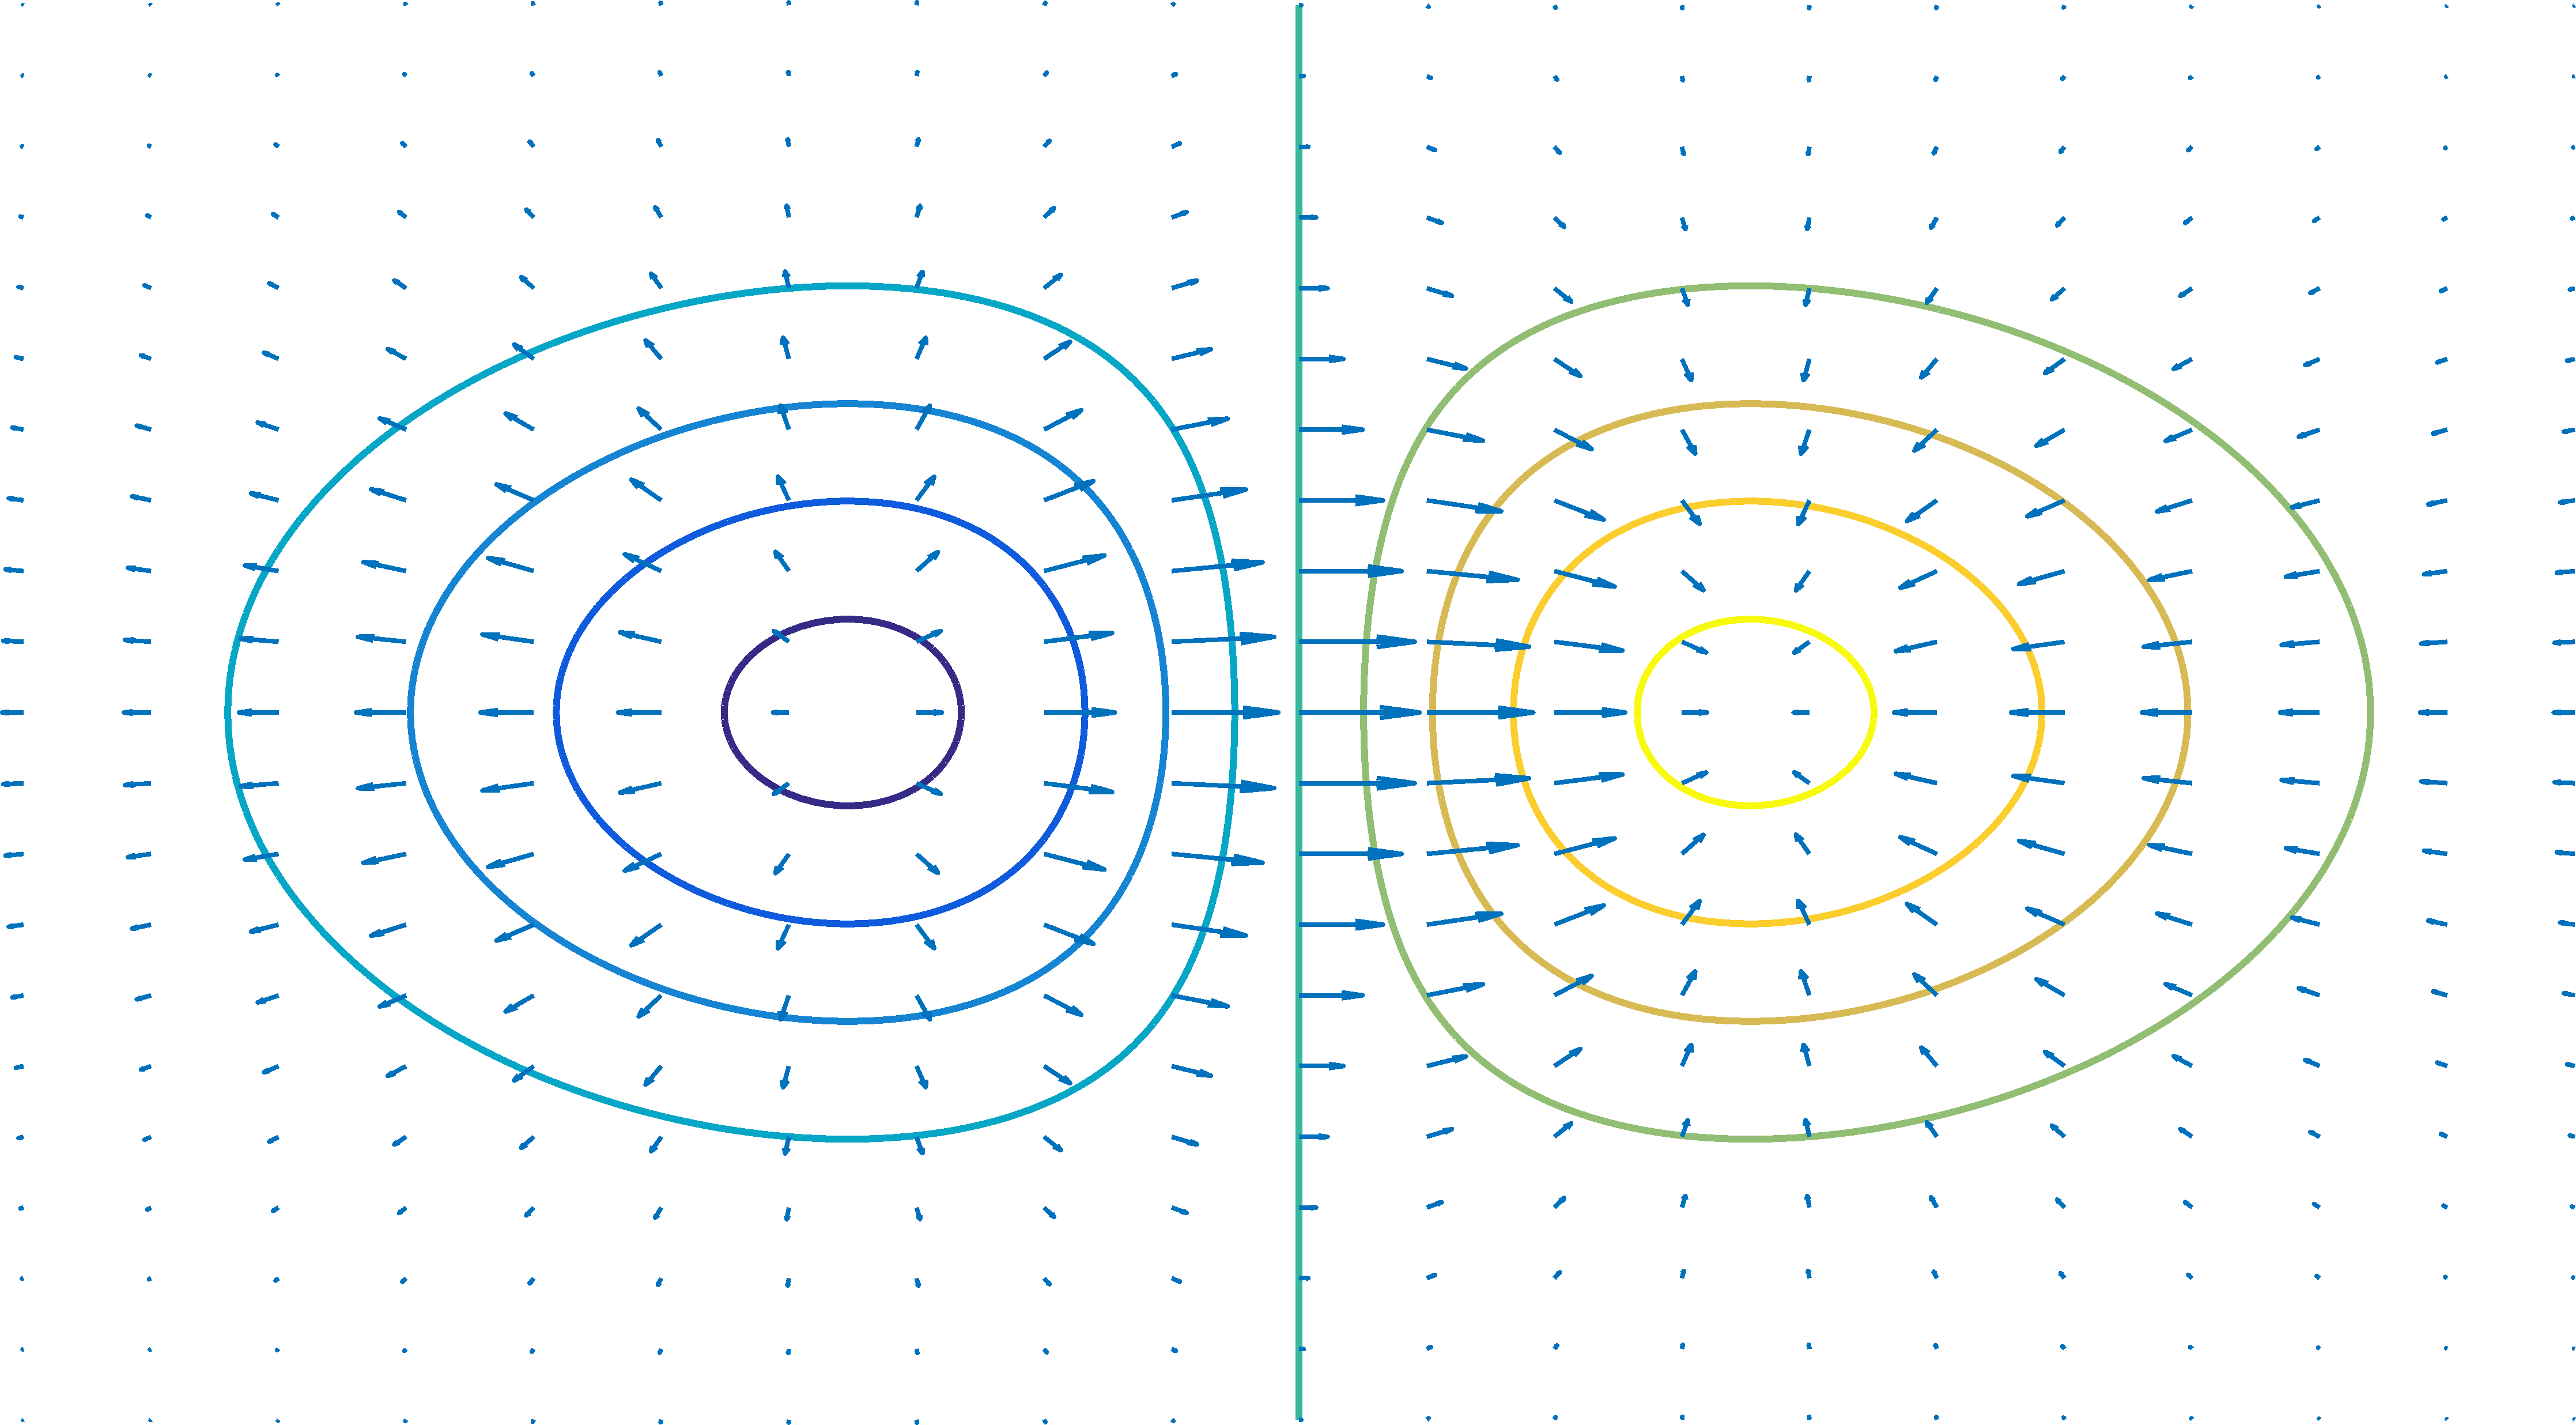
\includegraphics[width=\textwidth]{../Pictures/Front_image.png}
\end{figure}
\vskip2cm    
{\bfseries\LARGE
         Thomas E. Woolley\\       
    }
    \vfill
    Last edited on: \today }

{\let\cleardoublepage\clearpage 
\tableofcontents
} 

\chapter{Introduction}
In this course we will be concerned with ordinary differential equations, ODEs.

\begin{defin}
An ordinary differential equation (ODE) is a differential equation containing one or more functions of \underline{\textbf{exactly one}} independent variable and its derivatives.
\end{defin}

ODEs relate the change of one variable to changes in another variable and can be used to model and understand a wide variety of phenomena, such as projectile motion, animal population interactions and the progression of chemical reactions.

In these notes we consider two important aspects in the theory of ordinary differential equations. Specifically, we seek to
\begin{enumerate}
\item develop methods of modelling physical phenomena;
\item understand the properties of the equations without explicitly solving them.
\end{enumerate}

Point 2 may seem counter-intuitive as we have a variety of techniques that enable us to solve ODEs in closed form. Further, even if an explicit solution is not available, we can use numerical simulations to illustrate the dynamics of the ODEs. However, direct solutions are not always possible and, even when they are, they may not always enable clear interpretations and understanding of the underlying system. Equally, our analytical techniques will give us confidence in the solutions produced by numerical software.

Critically, what we gain in analytical specificity, we lose in global accuracy. Namely, we are going to learn techniques that will allow us to rigorously examine small regions of the ODE space at the expense of losing knowledge of the global dynamics. However, by the end of the course we will be able to patch together multiple parts of the local analysis in order to give us an approximate understanding of the entire dynamical system.

\section{Preliminary definitions}
We will be considering the rate of change of a variable, $u$, with respect to another variable, $t$. This dependence will be denoted
\bb
u(t).
\ee
Here, $u$ is a scalar function (\ie one-dimensional), but more generally, we will be considering systems of variables
\bb
\bm{u}(t)=\l u_1(t),u_2(t),\dots,u_k(t)\r.
\ee
On the board we will usually write bold symbols with an underline\footnote{I was once told that we use underlines to illustrate bold variables because when typesetting a document an underline would tell the printer that that symbol needed to be bold. However, if this is true, how did the writer indicate that they wanted a symbol underlined?} as it is easier to see, thus, $\bm{u}=\underline{u}$.

The values of $u$ or $\bm{u}$ define quantities of interest. For example they could be an animal population density, a distance or a speed. Further, $t$ can be any variable which these quantities are dependent on. Generally, however, we will take $t$ to be time and we will be considering how these values temporally evolve.

In order to link the changes in these quantities we define a system of ODEs in the most general way possible,
\bb
\bm{F}\l t,\bm{u},\frac{\rd \bm{u}}{\rd t},\frac{\rd^2 \bm{u}}{\rd t^2},\dots,\frac{\rd^n \bm{u}}{\rd t^n}\r=0,
\ee
with initial condition given by
\bb
\bm{u}(0)=\bm{u}_0.
\ee
Note that the initial condition is kept general as we will usually be interested in how the dynamics of the system change for different starting points.

\begin{example}[frametitle=Bacteria population growth]
\label{Expo_growth}
\COL{In this case we are only considering one population, thus, $\bm{u}=u$ and we specify $u(t)$ to be the population of E.Coli at time $t$. Initially, the population is $u_0$ and resources are abundant, thus, each E.Coli is able to double itself at a rate $r$/s. Explicitly, the population grows at a rate proportional to the population already present, \ie
\bb
\frac{\rd u}{\rd t}=ru.
\ee
This equation can be trivially solved to give
\bb
u(t)=u_0\exp(rt),\label{Intro_exp}
\ee
see \fig{Exponential}.

Note instead of specifying the time at which a population takes an arbitrary value, we can consider the more general time scale of how long does it take the population to double? Namely, at what point, $t_2$, is $u(t_2)=2u_0$. Rearranging \eqn{Intro_exp} we derive that
\bb
t_2=\frac{1}{r}\log\l 2\r.
\ee

Critically, once a model is constructed and an answer is found, we must consider whether if it is a good model or not. Clearly this model has problems because it predicts the population will grow exponentially quickly, without bound. The key problematic assumption that we have made is that the resources (\eg space, nutrients, etc.) do not run out. Although this may be a fine assumption to begin with, eventually the bacteria will be limited by competition.}
%\begin{figure}[!!!h!!!tb]
{\centering
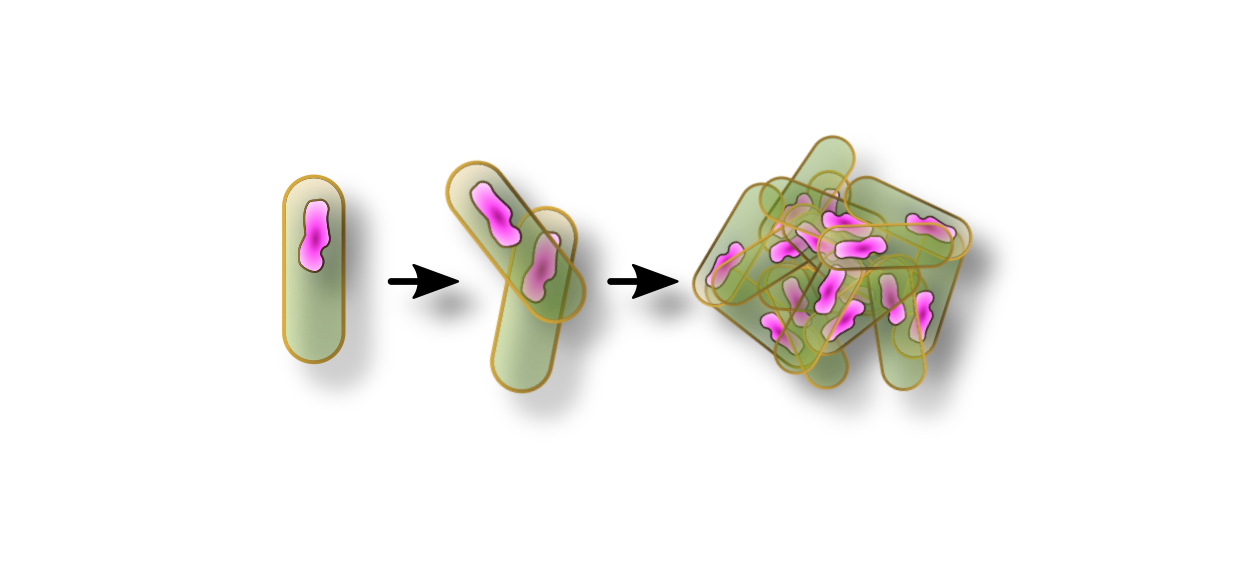
\includegraphics[width=\textwidth]{../Pictures/Bacteria.png}}
%\end{figure}
\end{example}


\begin{example}[frametitle=Bacteria and nutrient populations.]\label{Logi_growth}
\COL{Imagine a case similar to the one above, but we introduce a nutrient population, $v$. We assume that a bacterium can divide at a rate $r$ if and only if it can interact with enough nutrient. However, the nutrient is depleted at a rate $r$ as the bacteria interacts with it.

Here, the equation governing this system is going to be provided. However, later on we will learn how to write down and interpret interaction equations of the form
\bb
u+v \stackrel{r}{\longrightarrow} 2u.
\ee

The governing equations are
\begin{align}
\frac{\rd u}{\rd t}&=ruv,\quad u(0)=u_0,\label{Pop_u}\\
\frac{\rd v}{\rd t}&=-ruv,\quad v(0)=v_0.
\end{align}}
\COL{We notice that we can add the two equations and integrate to provide a conserved quantity,
\bb
u+v=c.\label{Conserved_c}
\ee
We can substitute \eqn{Conserved_c} into \eqn{Pop_u} to get
\bb
\frac{\rd u}{\rd t}=ru(c-u).\label{Log_1}
\ee
This is known as the logistic equation and we will see it many times throughout these notes, it is a simple example of competition between species for resources.}

\COL{Using partial fractions, we can directly solve \eqn{Log_1}. Specifically,
\begin{align}
\frac{\rd u}{\rd t}&=rcu\l 1-\frac{u}{c}\r,\nonumber\\
\Rightarrow\int_0^T\frac{\rd u}{u(1-u/c)}&=\int_0^Trc \rd t,\nonumber\\
\Rightarrow\int_0^T \frac{1}{u}+\frac{1/c}{1-u/c}  \rd u&=rcT,\nonumber\\
\Rightarrow\left[\ln(u)-\ln\l 1- \frac{u}{c} \r \right]^T_0&=rcT,\nonumber\\
\Rightarrow\ln\l\frac{u}{1- \frac{u}{c}} \r-\ln\l\frac{u_0}{1- \frac{u_0}{c}} \r&=rcT,\nonumber\\
\Rightarrow u(T)=\frac{c}{1+\frac{c-u_0}{u_0}\exp\l{-rcT}\r},
\end{align}
see \fig{Logistic}.

Comparing the models of bacteria growth, illustrated in \fig{Growth_examples}, we see that \eqn{Log_1} is a more realistic model for growth because there is a maximum population value which can be supported by the experiment. This maximum value is given by $c$ and is known as the carrying capacity. The parameter grouping $rc$ is also important as this control the time scale over which this maximum is obtained.}
\end{example}
\begin{figure}[!!!h!!!tb]
{\centering
\subfigure[\label{Exponential}]{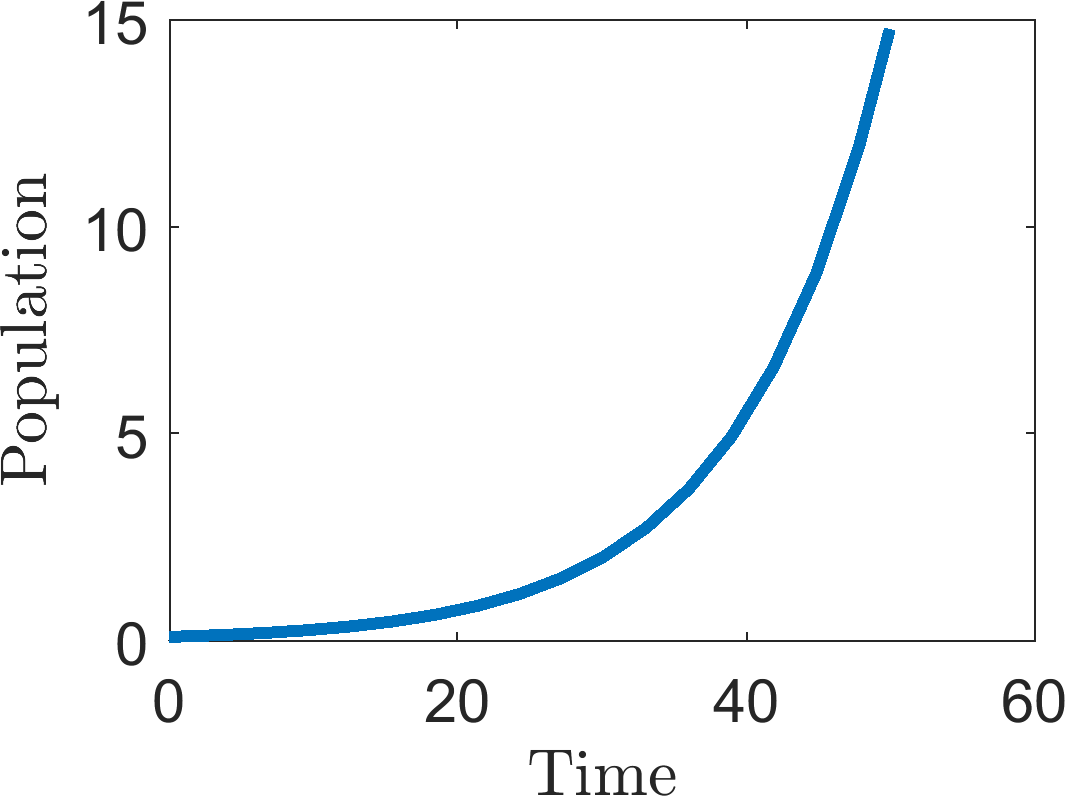
\includegraphics[width=\ttp]{../Pictures/Exponential.png}}
\subfigure[\label{Logistic}]{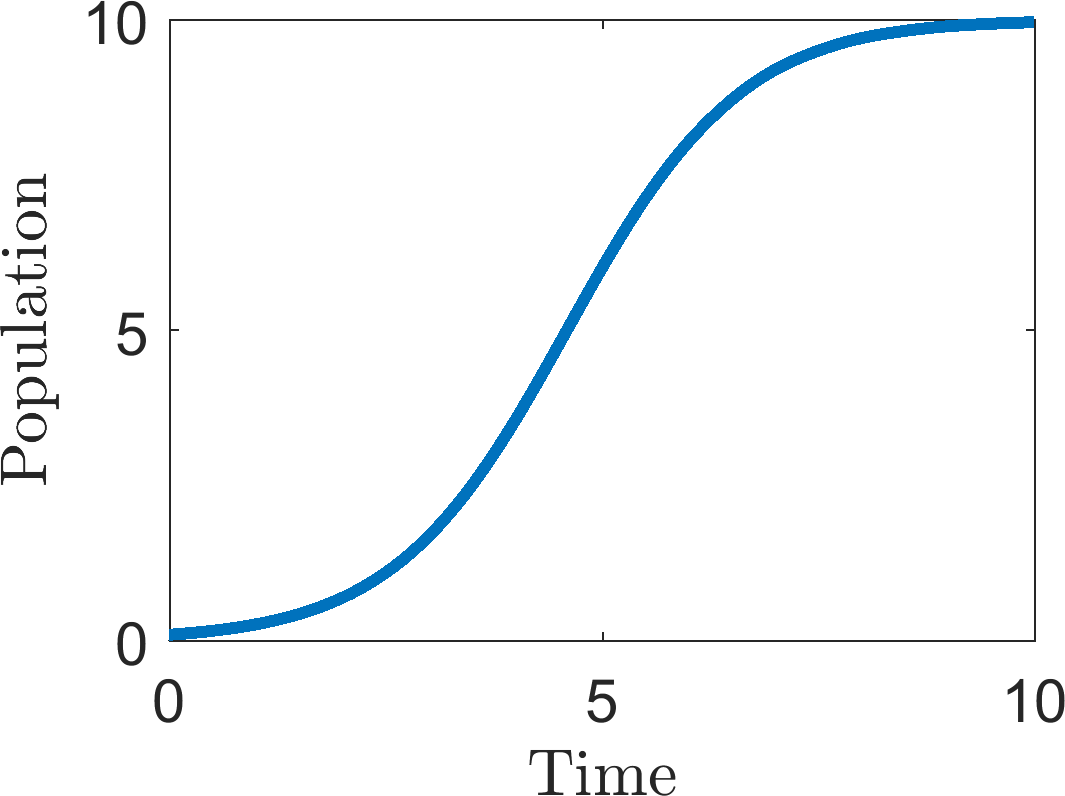
\includegraphics[width=\ttp]{../Pictures/Logistic.png}}
\caption{(a) Exponential growth. Parameters are $r=u_0=0.1$. See example \ref{Expo_growth}. (b) Logistic growth. Parameters are $c=10$, $r=u_0=0.1$. See example \ref{Logi_growth}.}\label{Growth_examples}}
\end{figure}


\begin{example}[frametitle=Duffing's equations.]\label{Duffing_example}
For our last example, consider the Duffing oscillator. The equation is simply a toy example that can be used to examine complex phenomena in a simple equation. In terms of interpretation, you can think of the equation as modelling the displacement of a beam near two magnetics. Critically, the beam and magnets are being forced to oscillate with amplitude $\gamma$ and frequency $\omega$ \see{Duffing_beam}.
\bb
\underbrace{\frac{\rd^2 x}{\rd t^2}}_{\textrm{Acceleration}}+\underbrace{2\delta\frac{\rd x}{\rd t}}_{\textrm{Air resistance}}+\underbrace{\beta x+\alpha x^3}_{\textrm{Beam's restorative force}}=\underbrace{\gamma\cos(\omega t)}_{\textrm{Forcing term}}.\label{Duffing_eqn}
\ee

We are not going to try and analytically solve or analyse Duffing's equation. Instead, we illustrate the dynamics that the equation produces as the amplitude of oscillation, $\gamma$, increases. Specifically, as $\gamma$ is increased the system becomes chaotic \see{Duffing_equation}.
\end{example}
\begin{figure}[!!!h!!!tbp]
\centering
\subfigure[\label{Duffing_beam}]{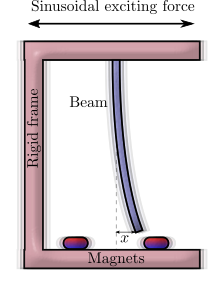
\includegraphics[width=.3\textwidth]{../Pictures/Duffing_beam.png}}
\subfigure[\label{Duffing_equation}]{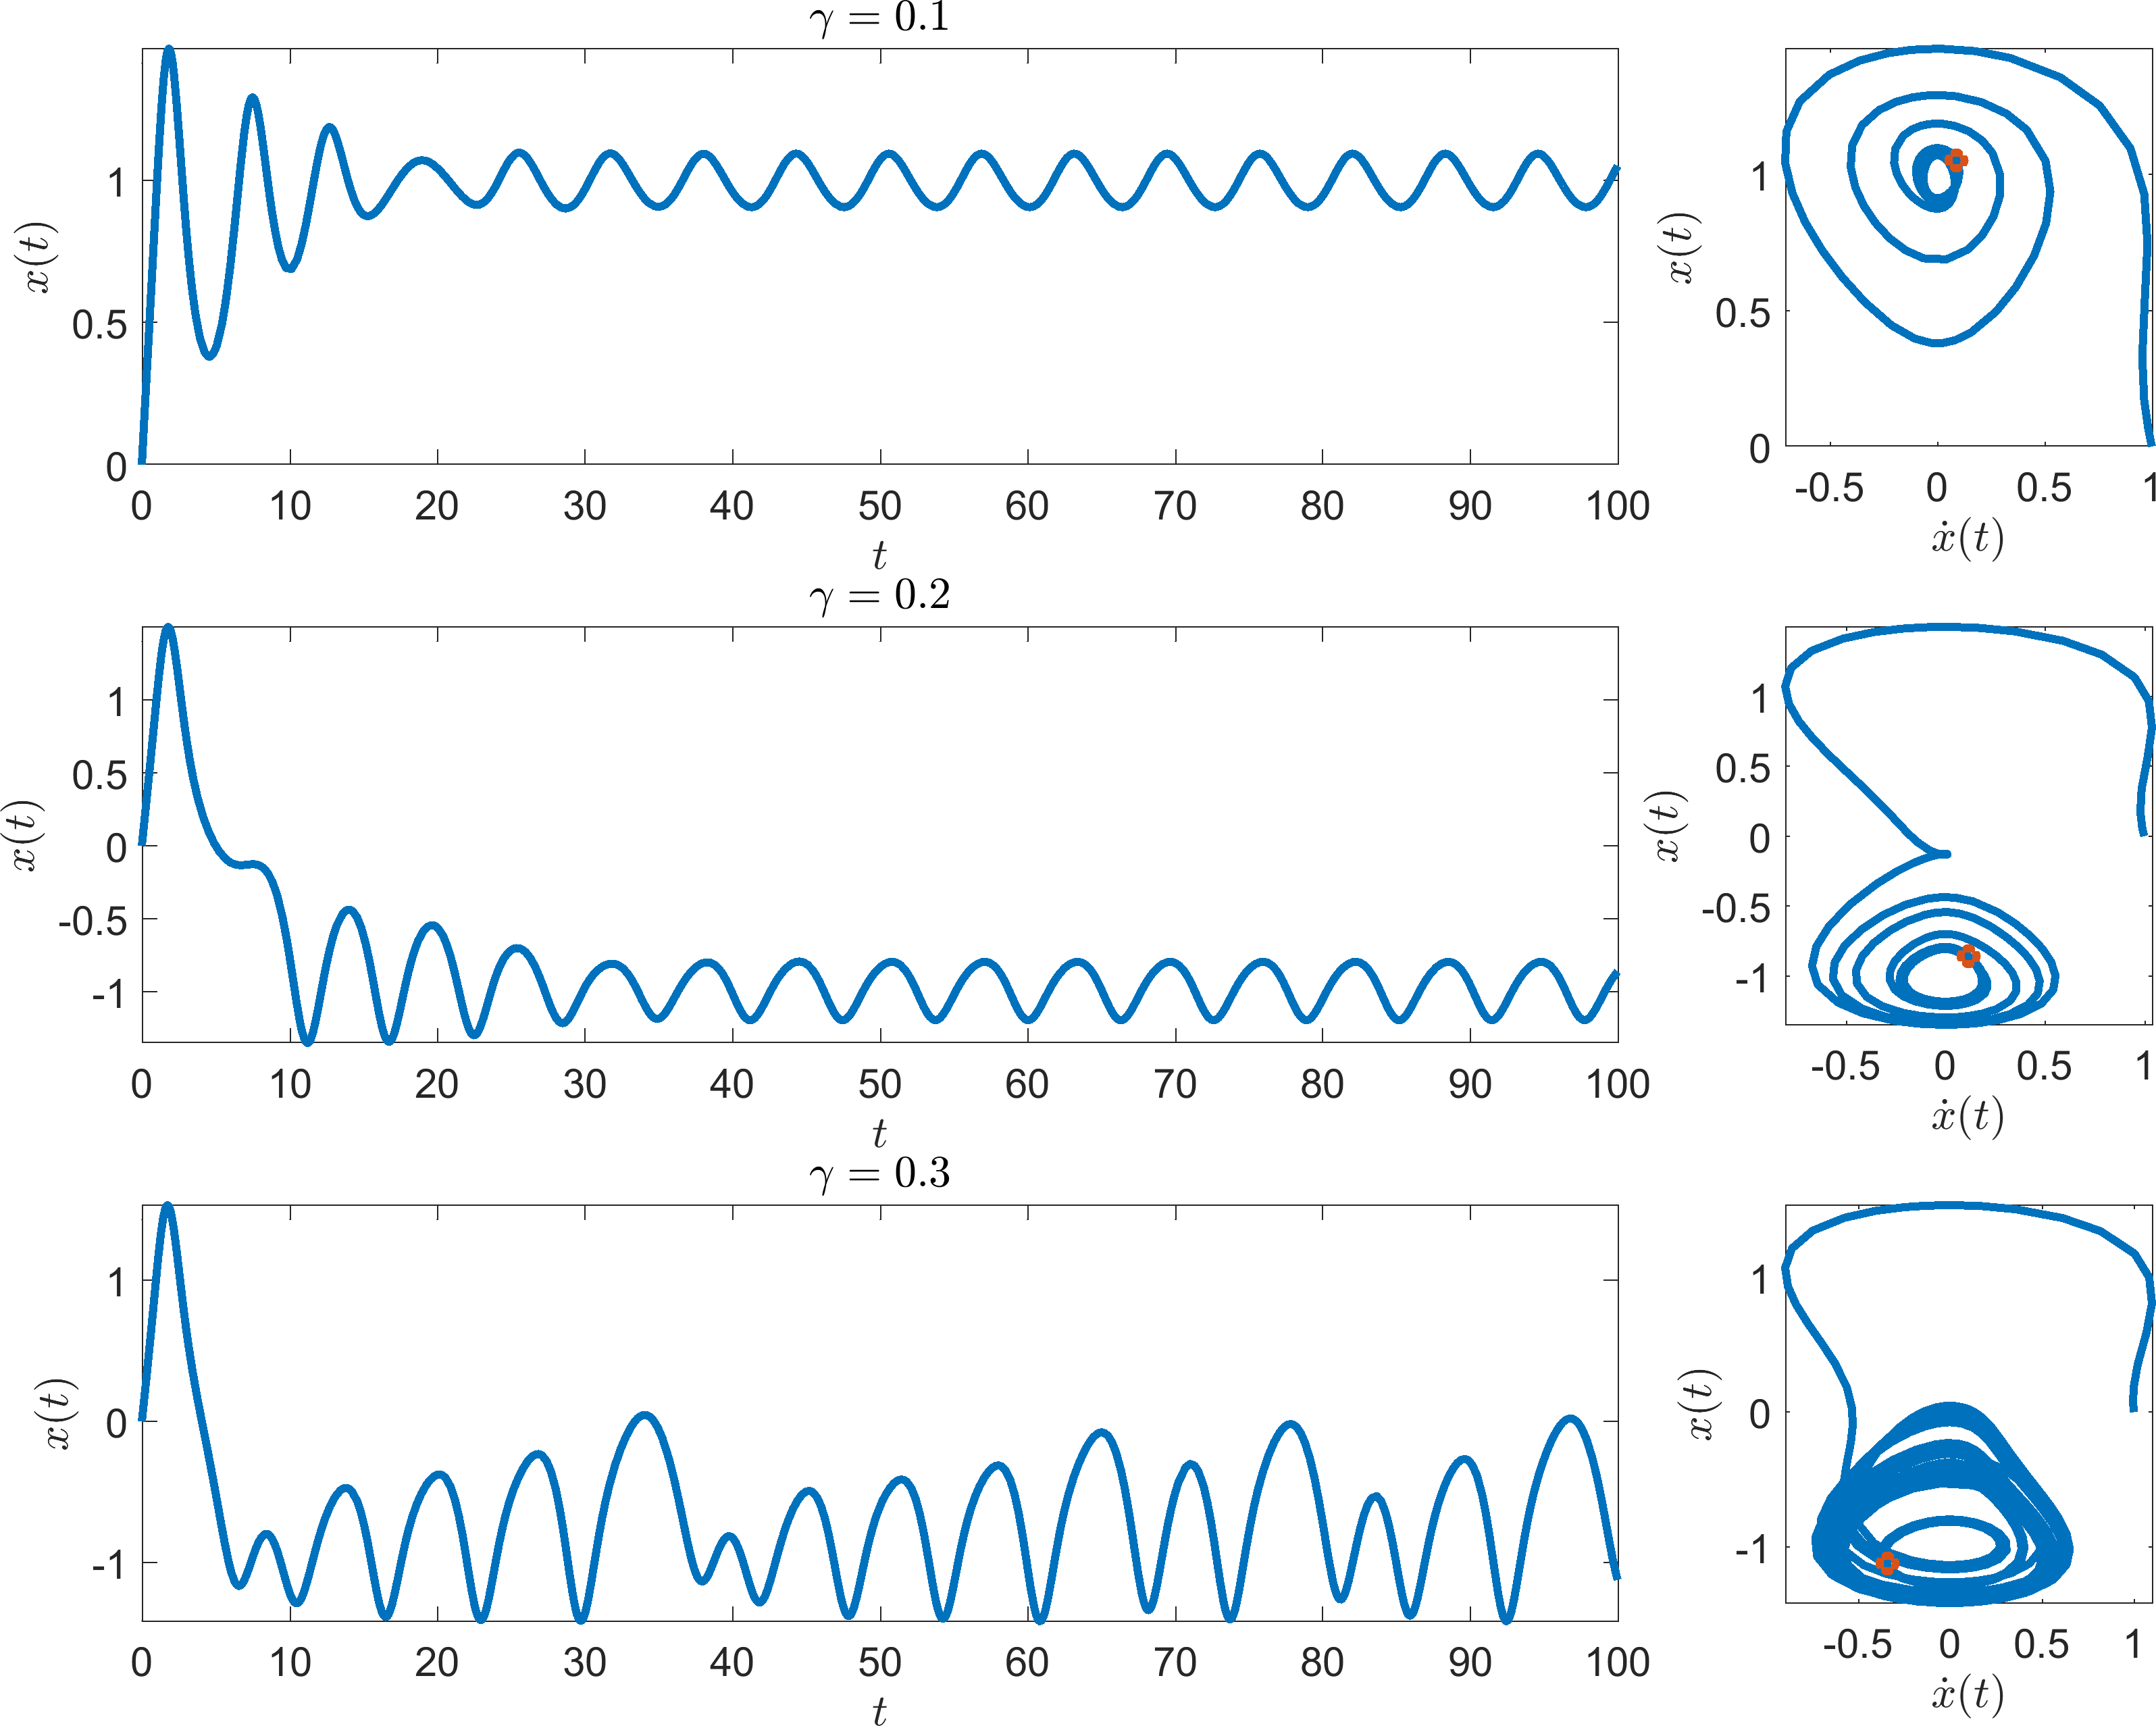
\includegraphics[width=\textwidth]{../Pictures/Duffing.png}}
\caption{\label{Duffing}(a) Schematic diagram of the system underlying Duffing's equation. (b) Three simulations of \eqn{Duffing_eqn} with increasing values of $\gamma$.}
\end{figure}

\begin{defin}
The \textbf{order} of a differential equation is the value of the highest derivative in the equation.
\end{defin}
Examples \ref{Logi_growth} and \ref{Expo_growth} are both first order equations, whilst example \ref{Duffing_example} is a second order equation. Generally (like polynomial equations of order) a differential equation of order $n$ will have $n$ linearly independent solutions.

\begin{defin}
A system of differential equations is \textbf{autonomous} if the system does not explicitly depend on the independent variable.
\end{defin}
When the variable is time, they are also called time-invariant systems, this simply means that we are assuming that the defined underlying laws of the system are identical to those for any point in the past, or future.

\begin{defin}
To save time we use a dot or prime mark to denote a derivative with respect to the argument, thus,
\bb
\dot{\bm{u}}(t)=\bm{u}'(t)=\frac{\rd \bm{u}}{\rd t}.
\ee
\end{defin}
Traditionally, dots are primarily used when the variable is time and primes are used otherwise. Note that higher orders derivatives are signified by the appropriate number of dots or primes. Namely, a second derivative would be denoted by two dots or primes, etc.

\begin{defin}
A \textbf{trajectory} is a solution, $u(t)$.
\end{defin}
The graphs in \figs{Growth_examples}{Duffing} illustrate single trajectories of their respective systems.



In this course we are going to occupy ourselves with systems of autonomous first order equations, of the form
\bb
\frac{\rd \bm{u}}{\rd t}=\dot{\bm{u}}=\bm{F}(\bm{u}).\label{ODE}
\ee
This may seem highly restrictive. However, systems of first order equations can have extremely complicated properties, such as oscillations and chaos, which we will try to understand.

\COL{Critically, equations of higher order can be written as a system of first order equations. For example, if
\bb
\bm{G}\l \bm{u},\frac{\rd \bm{u}}{\rd t},\frac{\rd^2 \bm{u}}{\rd t^2},\dots,\frac{\rd^n \bm{u}}{\rd t^n}\r=0
\ee
then we can define $n-1$ new equations of the form $\bm{v}_1=\rd \bm{u}/\rd t$ and $\bm{v}_i=\rd \bm{v}_{i-1}/\rd t=\rd^{i} \bm{u}/\rd t^{i}$ for $2\leq i \leq n-1$ to produce the first order system
\begin{align}
&\bm{G}\l \bm{u},\bm{v}_1,\dots,\bm{v}_{n-1},\frac{\rd \bm{v}_{n-1}}{\rd t}\r=0,\\
&\frac{\rd \bm{u}}{\rd t}=\bm{v}_1,\\
&\vdots\nonumber\\
&\frac{\rd \bm{v}_{n-2}}{\rd t}=\bm{v}_{n-1}.
\end{align}}
\begin{example}[frametitle=Duffing's equations without forcing.]\label{Duffing_example2}
\COL{Setting $\gamma=0$ in Duffing's equation and letting
\bb
v=\frac{\rd x}{\rd t}
\ee
then we are able to convert the single second order equation seen in \eqn{Duffing_equation} to two first}\COL{ order ODEs,
\begin{align}
\frac{\rd v}{\rd t}&=-2\delta v-(\beta x+\alpha x^3)\\
\frac{\rd x}{\rd t}&=v.
\end{align}
Note that $v$ is an apt variable name for the variable, because, as discussed in example \ref{Duffing_example}, $x$ can be thought of as position, making $v$ a velocity.}
\end{example}
\begin{thm}
A solution trajectory, $\bm{u}(t)$, of \eqn{ODE} cannot self-intersect \see{Trisectrix}.
\end{thm}
\begin{proof}
\COL{Suppose there is an intersection. Hence, there exist two points, $t_1$ and $t_2$, such that $\bm{u}(t_1)=\bm{u}(t_2)$ then we will also have that $\bm{F}(\bm{u}(t_1))=\bm{F}(\bm{u}(t_2))$. However, the curves intersect, thus, the curves must be travelling in different directions at $t_1$ and $t_2$ \see{Intersect}, meaning that the derivatives are different there, \ie $\dot{\bm{u}}(t_1)\neq\dot{\bm{u}}(t_2)$. But
\bb
\dot{\bm{u}}(t_1)=\bm{F}(\bm{u}(t_1))=\bm{F}(\bm{u}(t_2))=\dot{\bm{u}}(t_2),
\ee
which produces a contradiction. Hence the curves cannot intersect.}
\end{proof}
\begin{figure}[!!!h!!!tb]
\centering
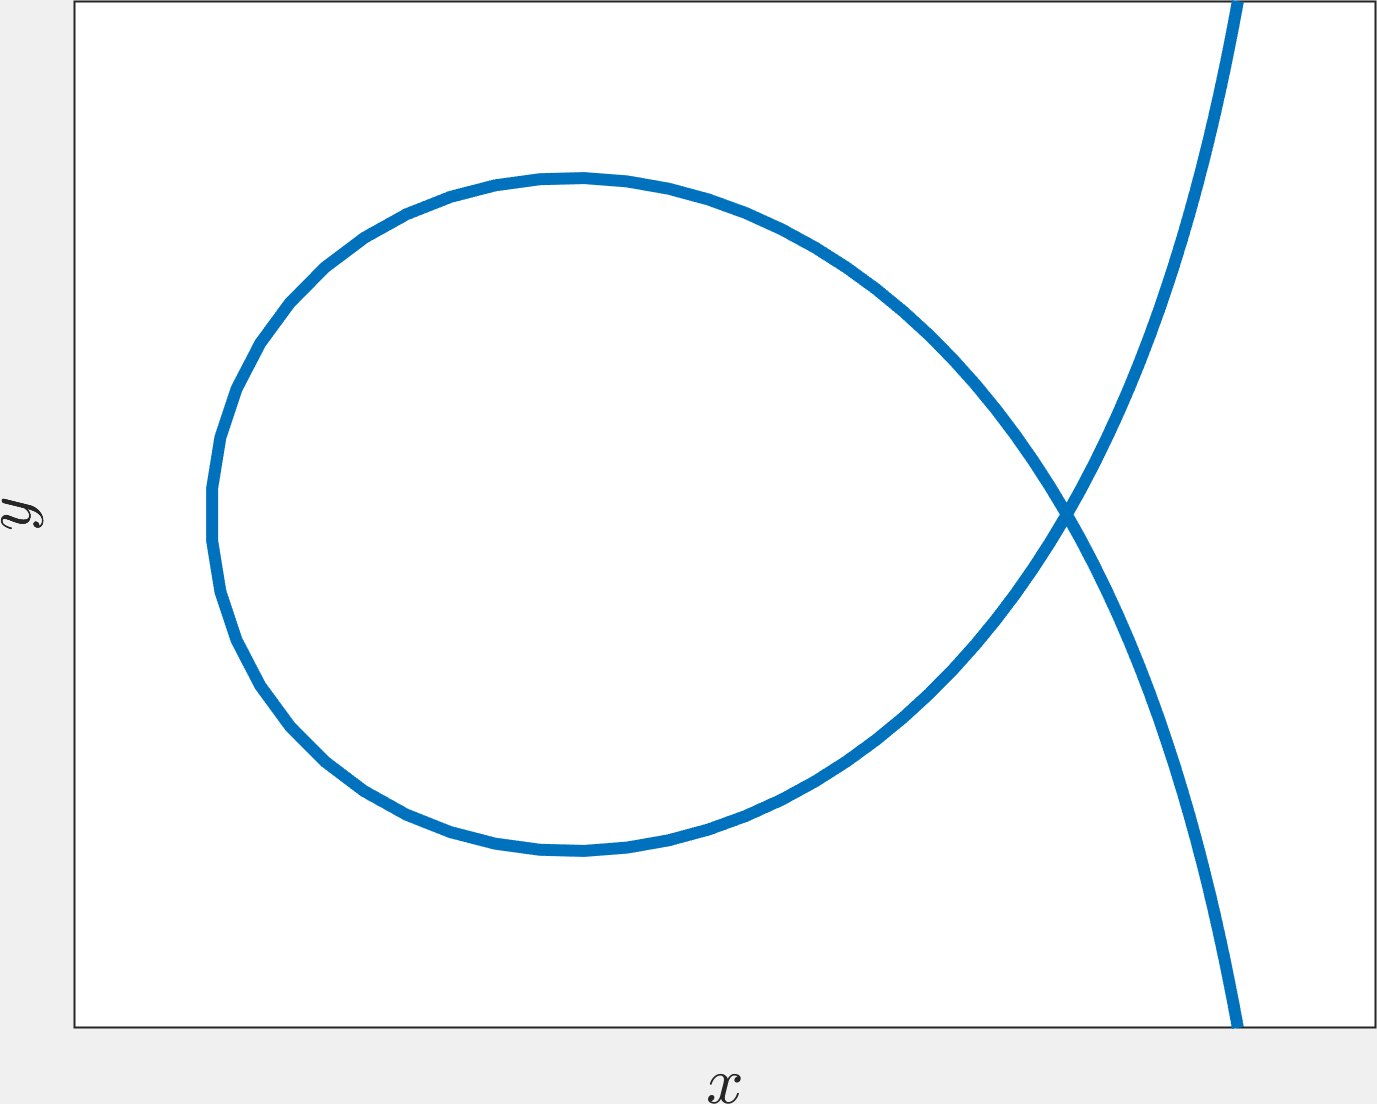
\includegraphics[width=\ttp]{../Pictures/Trisectrix.png}
\caption{\label{Trisectrix} A solution of \eqn{ODE} cannot look like this.}
\end{figure}


\subsection{Existence and uniqueness}
With this being an applied mathematics course we are often very `fast and loose' with our rigour. However, it is good to know that theorems have been proven regarding the existence and unique of solution to \eqn{ODE}. Here we will quote the theorem in one dimension, but the theorem can be expanded to any number of variables.
\begin{thm}Existence-Uniqueness theorem.

Suppose the function $F(u)$ is differentiable and the derivative, $F'(u)$, is continuous for all values of $u$ then there will exist some constant $c>0$ such that
\bb
\dot{u}=F(u),\quad u(t_0)=u_0,
\ee
has a solution and it is guaranteed to exist and be unique in some finite time interval $|t-t_0|<c$.\label{Existence_Uniqueness}
\end{thm}
Note that:\COL{
\begin{itemize}
\item we will not consider the proof here. For those who are interested look up ``Picard's theorem''. Picard's theorem is actually weaker than the one specified above, but theorem \ref{Existence_Uniqueness} expresses the statement in the most useful form for us.
\item in many cases solutions will exist and be unique for all time, but, the theorem hardly ever provides an optimal value for $c$. However, the theorem is general enough to include cases where `blow up' occurs. Namely, blow up occurs when a solution tends to infinity in finite time.
\item without loss of generality we can always take $t_0=0$ (why?). \textbf{This is only true in autonomous systems}.
\item solution curves cannot intersect, otherwise there would be two different solutions going through the same point and there would not be uniqueness around the intersection \see{Intersect}.
\item the case for higher dimensional systems is effectively the same except we need the function
\bb
\bm{F}(\bm{u})=\left(
\begin{array}{c}
{F_1}(u_1,u_2,u_3,\dots,u_n)\\
{F_2}(u_1,u_2,u_3,\dots,u_n)\\
\vdots\\
{F_n}(u_1,u_2,u_3,\dots,u_n)
\end{array}
\right)
\ee to be continuous in all of its derivatives.
\end{itemize}}
\begin{figure}[!!!h!!!tb]
\centering
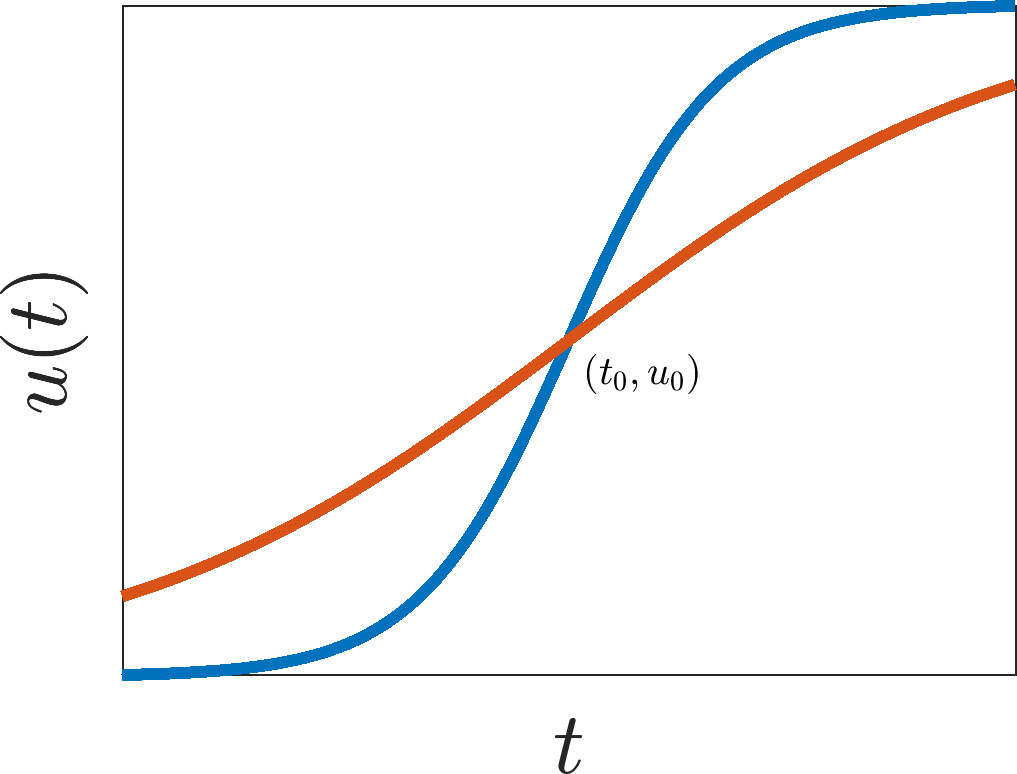
\includegraphics[width=\ttp]{../Pictures/Intersection.png}
\caption{\label{Intersect}Two different solution curves of a one-dimensional ODE cannot intersect.}
\end{figure}

\begin{defin}\label{Monotonic_def}
A differentiable function is \textbf{monotonic} if its derivative never changes sign. Moreover, the function is monotonically increasing (decreasing) if the derivative is positive (negative).
\end{defin}
\begin{defin}\label{Strict_monotonic_def}
A differentiable function is \textbf{strictly monotonic} if its derivative never changes sign and is never zero.
\end{defin}
See \fig{Monotonics} for examples of definitions \ref{Monotonic_def} and \ref{Strict_monotonic_def}.
\begin{figure}[!!!h!!!tb]
\centering
\subfigure[\label{Non_monotonic}]{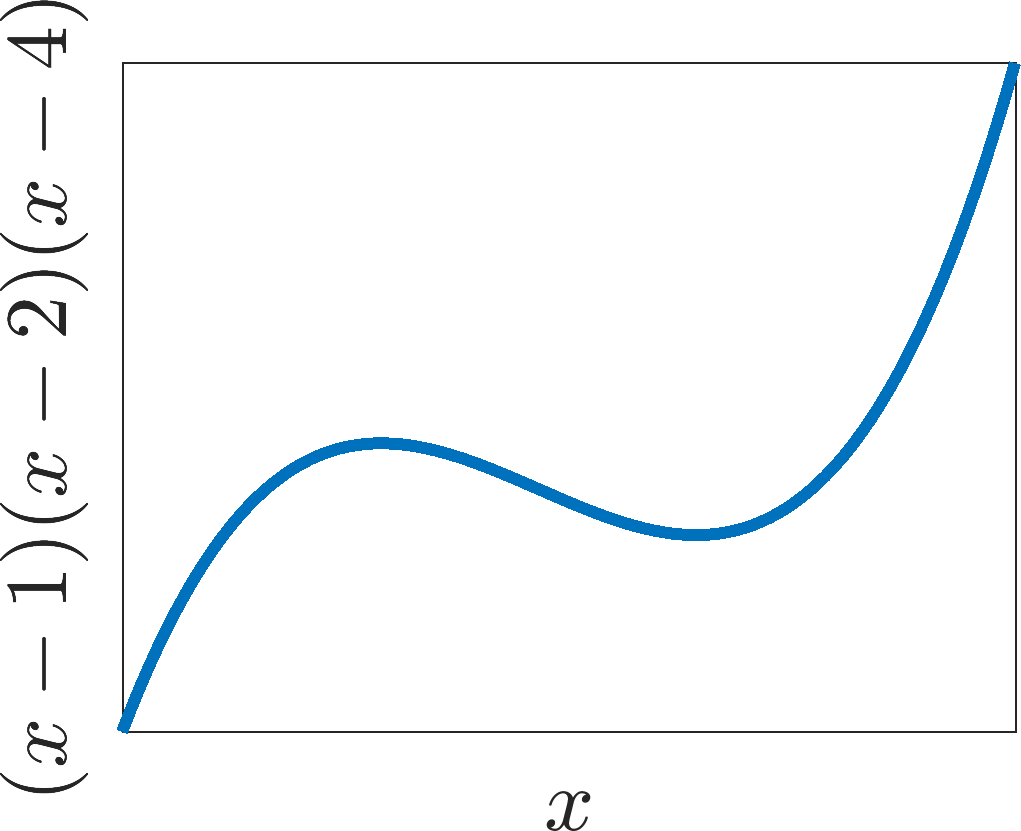
\includegraphics[width=\tttp]{../Pictures/Non_monotonic.png}}
\subfigure[\label{Monotonic}]{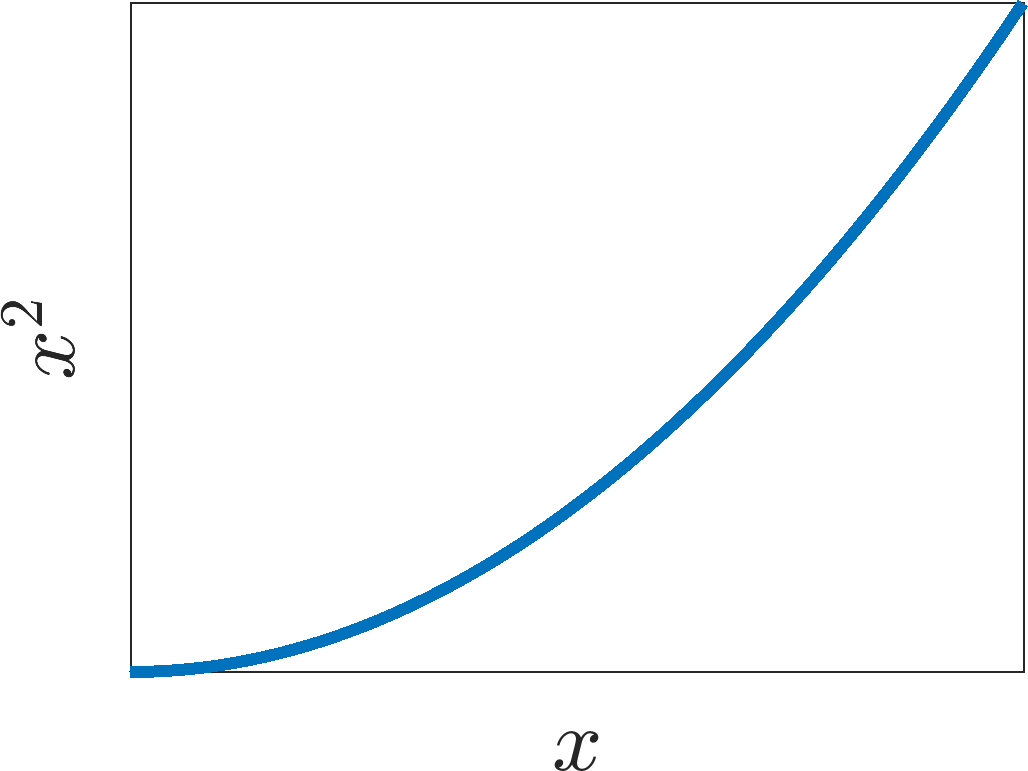
\includegraphics[width=\tttp]{../Pictures/Monotonic.png}}
\subfigure[\label{Strictly_monotonic}]{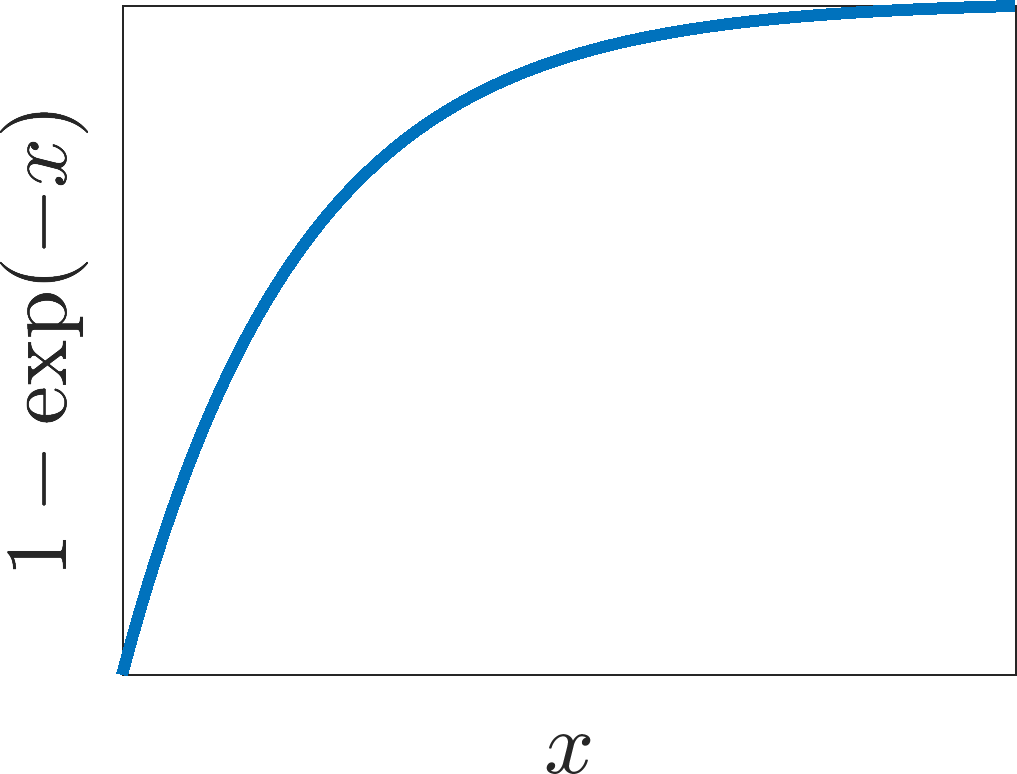
\includegraphics[width=\tttp]{../Pictures/Strictly_monotonic.png}}
\caption{\label{Monotonics}(a)\COL{ A non-monotonic function.} (b) \COL{A monotonic function.} (c) \COL{A strictly monotonic function.}}
\end{figure}


\begin{cor}
Suppose $F(u)$ is a scalar function that is continuously differentiable. The solution, $u(t)$, of the one dimensional ODE,
\bb
\dot{u}=F(u),\quad u(t_0)=u_0,
\ee
cannot oscillate. Specifically, $u(t)$ must either be constant, or a monotonically increasing, or decreasing function.
\end{cor}
\begin{proof}
\COL{Suppose that $u^*(t)$ is non-monotonic. By definition its derivative changes sign. By continuity there is somewhere, $t_c$, such that $\rd u^*(t_c)/\rd t=0$.
Thus, $u^*$ is a solution of
\bb
\dot{u^*}=F(u^*),\quad u^*(t_c)=u^*_c.\label{Starred}
\ee
Let us construct the constant function $u\equiv u^*_c$. We note that, $F(u^*(t_c))=0$ and, thus,  $u$ is also a solution to \eqn{Starred}. However, this means that we have two different solutions to \eqn{Starred} violating theorem \ref{Existence_Uniqueness}. By contradiction $u^*(t)$ has to be monotonic.}
\end{proof}
This means that to have oscillatory phenomena in a system either we need more than one population, or the system has to be non-autonomous. See example \ref{Duffing_example} for a case where both of these factors are present and do indeed produce oscillations (and chaos).



\section{Taylor expansions}
This section is to remind you of the Taylor expansion technique. The Taylor expansion is one of the most powerful tools for an applied mathematician because very often we want to know what happens to a trajectory near some critical point. Although the kinetics maybe very non-linear and difficult to understand globally we can use the Taylor expansion to simplify the dynamics in a small region around the critical point in order to gain knowledge about the dynamics in this region.

\begin{thm}\label{Taylor}
Suppose $f(x)$ is infinitely differentiable at a point $a$ then the Taylor series of $f$ at $a$ is the power series
\bb
f(x)=\sum _{n=0}^{\infty }{\frac{f^n(a)}{n!}(x-a)^n},
\ee
which is explicitly
\bb
f(x)=f(a)+{\frac {f'(a)}{1!}}(x-a)+{\frac {f''(a)}{2!}}(x-a)^{2}+{\frac {f'''(a)}{3!}}(x-a)^{3}+\cdots,
\ee
where $n!$ denotes the factorial of $n$ and $f^{(n)}(a)$ denotes the $n^{th}$ derivative of $f$ evaluated at the point $a$. The derivative of order zero of $f$ is defined to be $f$ itself and $(x-a)^0$ and $0!$ are both defined to be 1.
\end{thm}
\begin{example}[frametitle=Taylor expansions.]
\begin{itemize}
\item $\exp(x)$ at $x=0$ \see{Taylor_approximations}.
\COL{
\bb
\exp(x)=1+x+{\frac {1}{2}}{x}^{2}+{\frac {1}{6}}{x}^{3}+O \left( {x}^{4}
 \right) .
 \ee}
\item $\cos(x)$ at $x=0$.
\COL{
\bb
\cos(x)=1-{\frac {1}{2}}{x}^{2}+O \left( {x}^{4} \right) .
\ee}
\item $1/\l 1+x\r$ at $x=0$
\COL{
\bb
\frac{1}{1+x}=1-x+{x}^{2}-{x}^{3}+O \left( {x}^{4} \right) .
\ee}
\item $\sin(x)$ at $x=\pi/2$.
\COL{
\bb
\sin(x)=1-{\frac{1}{2}} \left( x-{\frac {\pi}{2}} \right) ^{2}+O \left( 
 \left( x-{\frac {\pi}{2}} \right) ^{4} \right)  .
\ee}
\end{itemize}
\end{example}
\begin{figure}[!!!h!!!tb]
\centering
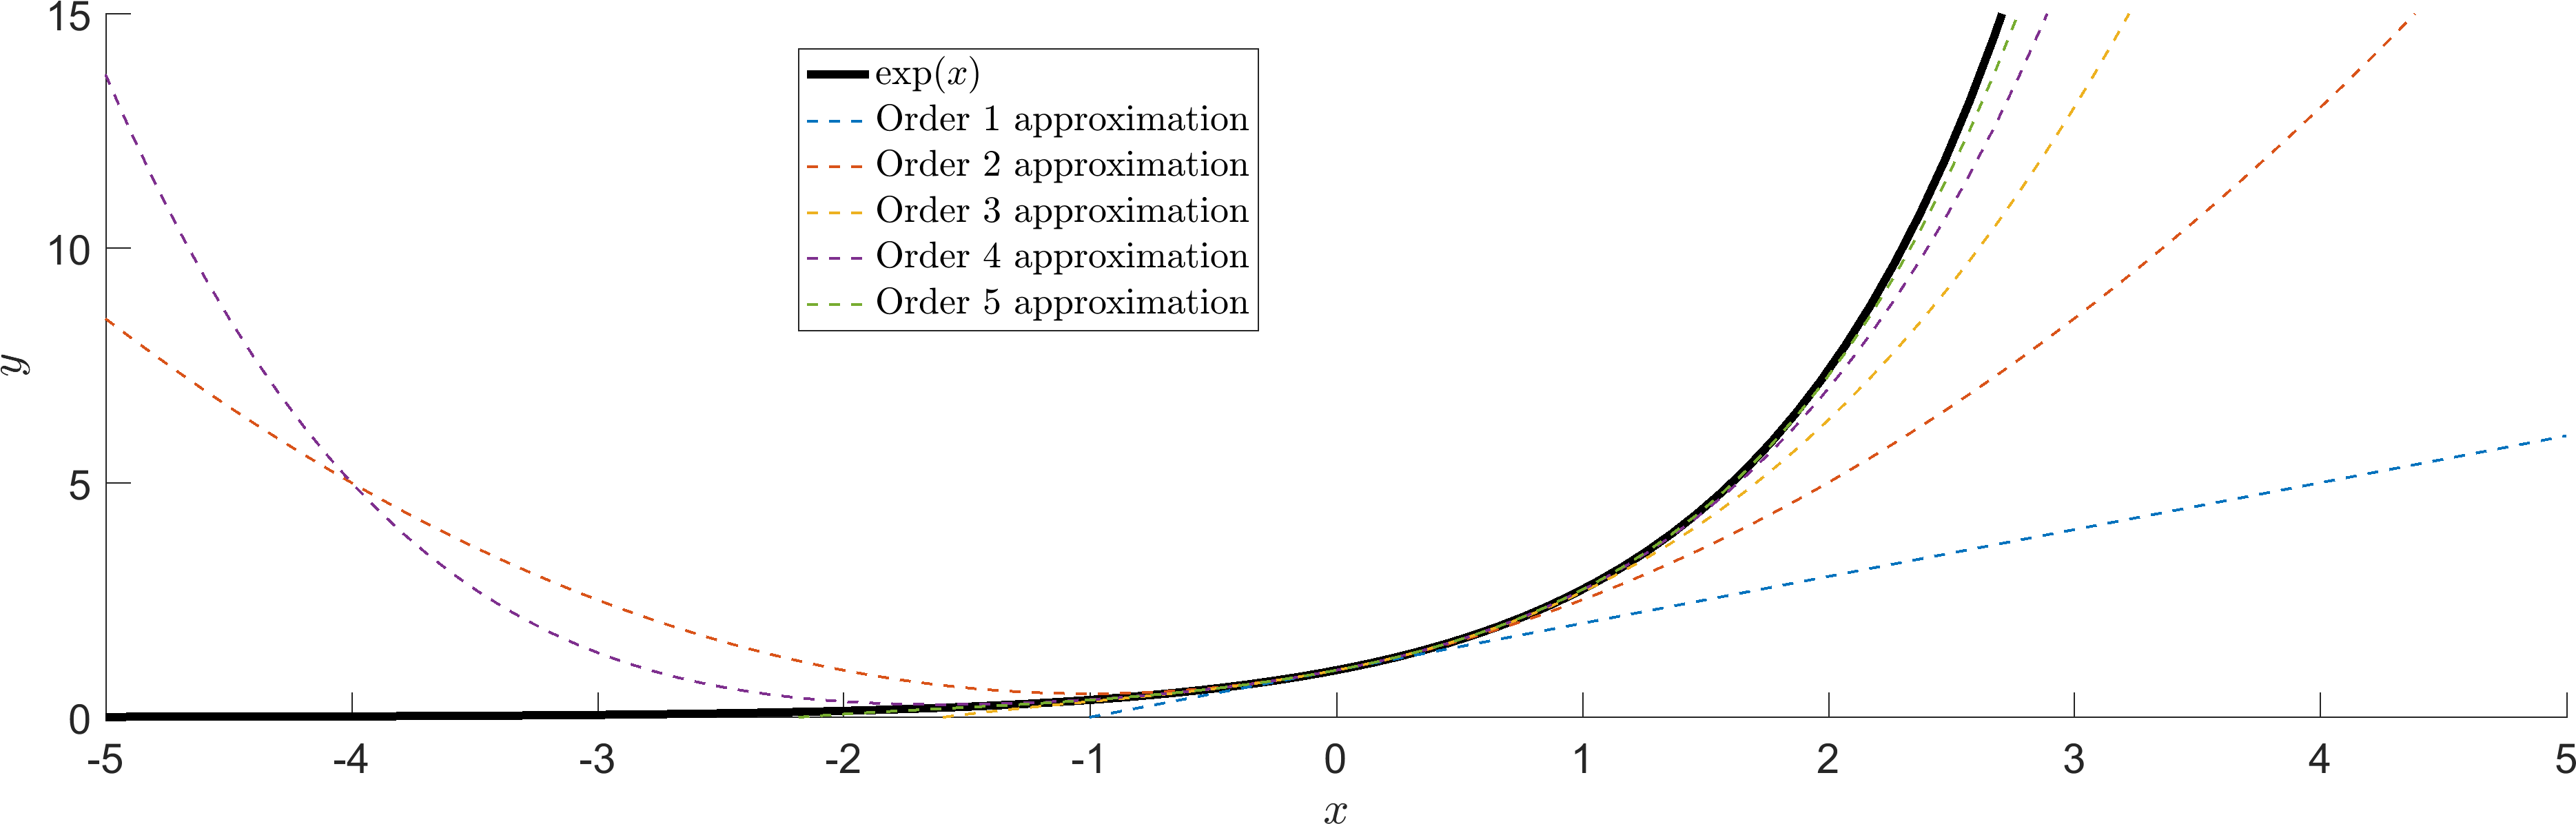
\includegraphics[width=\textwidth]{../Pictures/Taylor_approximations.png}
\caption{\label{Taylor_approximations} Approximating the exponential function with different orders of Taylor series.}
\end{figure}

\COL{Although Theorem \ref{Taylor} is the most general form of Taylor's theorem we are frequently going to want to know what happens near a specific point. Namely, if $x$ is the point of interest, what does the function look like at $x+\epsilon$, where $\epsilon \ll 1$. Specifically, this simply comes down to redefining $x\coloneqq x+\epsilon$ and $a\coloneqq x$ in Theorem \ref{Taylor}, namely
\bb
f(x+\epsilon)=f \left( x \right) +\epsilon{\frac {\rm d}{{\rm d}x}}f \left( x \right) 
+{\frac {{\epsilon}^{2}}{2}{\frac {{\rm d}^{2}}{{\rm d}{x}^{2}}}f \left( x
 \right) }+{\frac {{\epsilon}^{3}}{6}{\frac {{\rm d}^{3}}{{\rm d}{x}^{
3}}}f \left( x \right) }+O \left( {\epsilon}^{4}
 \right). 
\ee}\COL{
Since $\epsilon\ll 1$ we can truncate this series to obtain a good estimate after only a first term in $\epsilon$,
\bb
f(x+\epsilon)\approx f \left( x \right) +\epsilon{\frac {\rm d}{{\rm d}x}}f \left( x \right).
\ee
This is known as linearisation. You are taking the (possibly complicated) function $f$ and rewriting it as a linear function in $\epsilon$.}

Courses in the third year will deal with what information you get in the case that you truncate at $\epsilon^2$, or higher. This is non-linear analysis.

\subsection{Multivariate Taylor expansion}
A similar theorem can be stated when the function $f$ has more than one argument.
\begin{defin}
If $f$ is a function of more than one variable it is called \textbf{multivariate}.
\end{defin}

\COL{Here we simply state the expansion to first order expansion that we will be concerned with throughout the course.
\bb
f(x+\epsilon_1,y+\epsilon_2)\approx f(x,y)+\epsilon_1 f_x+\epsilon_2 f_y,
\ee
where we observe that we have used a subscript $f_x$ to denote the partial derivative $\partial f/\partial x$ and similarly for $f_y$.}
\begin{defin}
For brevity we use subscripts to stand for partial derivatives,
\bb
f_{x_1x_2\dots x_n}=\frac{\partial^n f}{\partial x_1\partial x_2\dots\partial x_n}.
\ee
\end{defin}
\begin{example}[frametitle=Multivariate Taylor expansion.]
\begin{itemize}
\item $\sin(x+y)$ at $x=y=0$.
\COL{
\bb
\sin(x+y)\approx x+y.
\ee}
\item $\sin(x)\cos(y)$ at $x=y=0$.
\COL{
\bb
\sin(x)\cos(y)\approx x.
\ee}
\end{itemize}
\end{example}

\section{Polar coordinates}
Many phenomena that we will model will fall under the consideration of spatial movement, for example in Chapter \ref{How to model a system} and question sheet two we will be considering planetary movement. Critically, in many of these cases the objects tend to move in circular trajectories orbiting a single point. Thus, it is more natural to use polar coordinates $(r,\theta)$ to describe the motion, rather than Cartesian coordinates $(x,y)$ \see{Polars}. However, it may be easier to model the system in Cartesian coordinates. Thus, we need to know how to convert between one set and another.
\begin{figure}[h!!!tb]
\centering
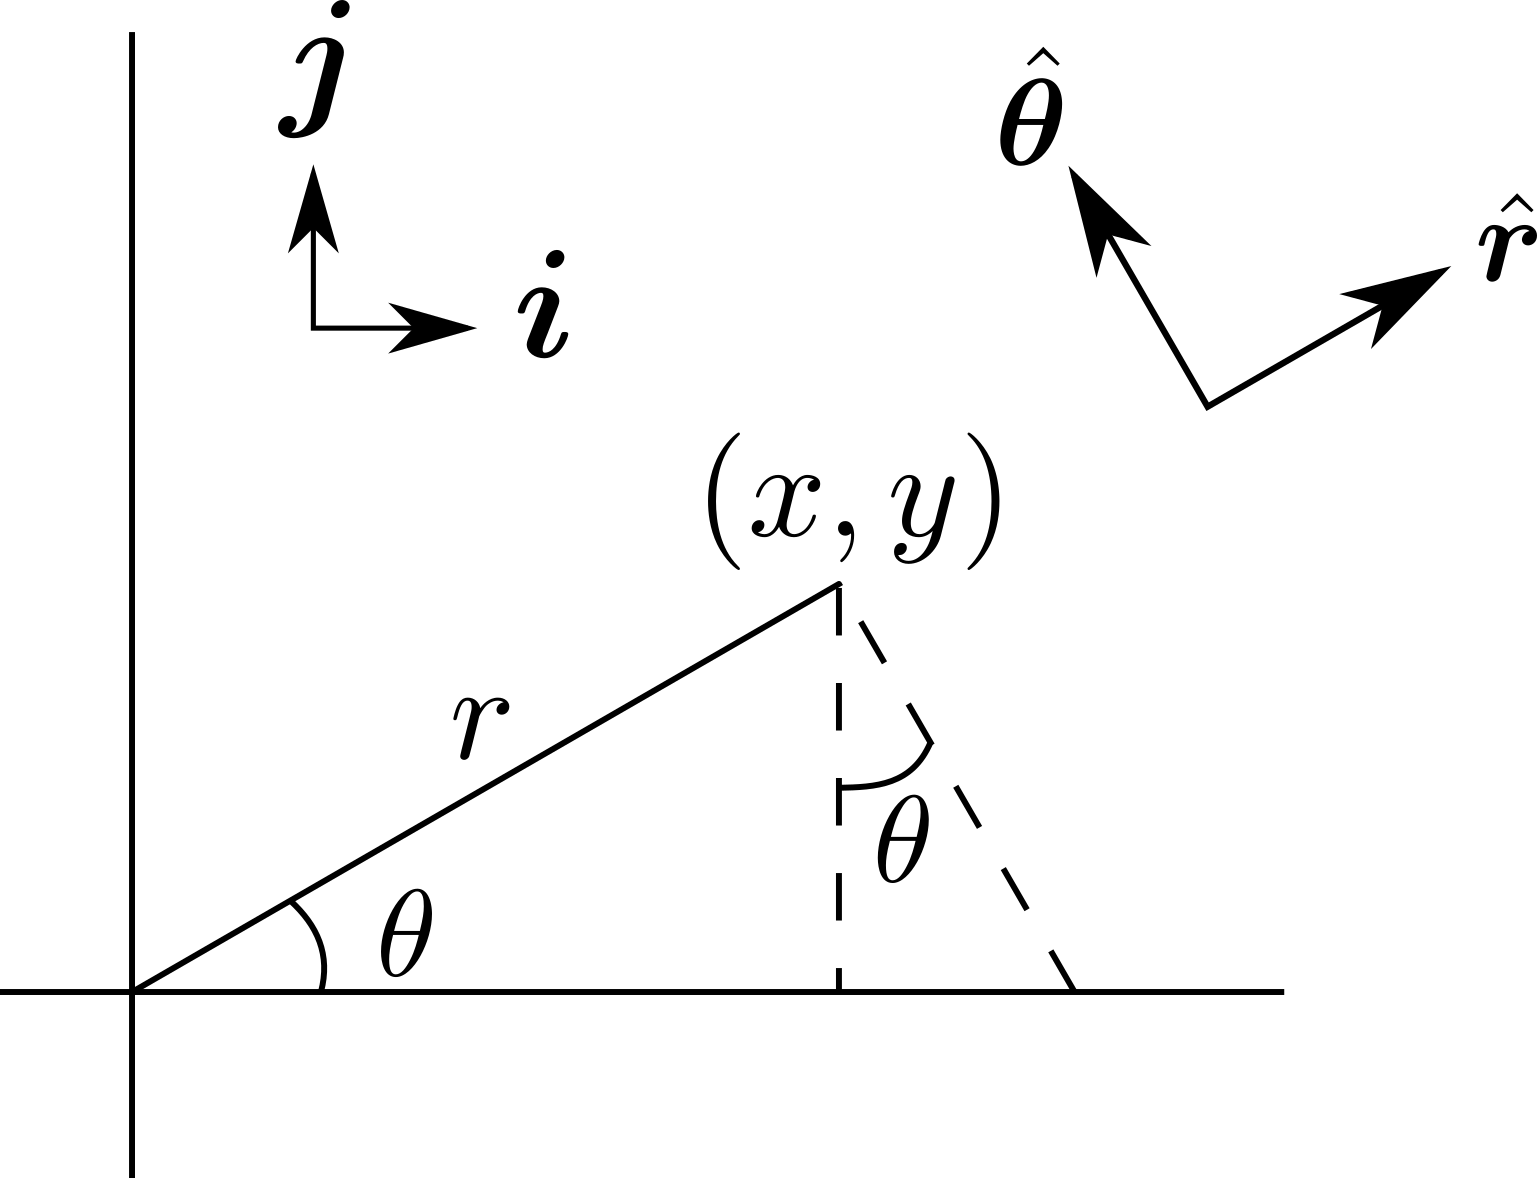
\includegraphics[width=\ttp]{../Pictures/Polars.png}
\caption{\label{Polars} Cartesian and polar coordinates.}
\end{figure} 

\fig{Polars} illustrates the fundamental relationships between the Cartesian and the polar coordinates, namely:
\begin{align}
x=r\cos(\theta),\\
y=r\sin(\theta).
\end{align}
Critically, these specify $x$ and $y$ singly as functions $(r,\theta)$. These, in turn, can be used to construct equations for $r$ and $\theta$ separately as functions of $(x,y)$, namely,
\bb
r^2=x^2+y^2,
\ee
and
\bb
\theta=\arctan\l\frac{y}{x}\r,\quad \textrm{or}\quad\theta=\arccos\l\frac{x}{\sqrt{x^2+y^2}}\r,\quad \textrm{or}\quad\theta=\arcsin\l\frac{y}{\sqrt{x^2+y^2}}\r.\label{theta_eqns}
\ee
where the appropriate function $\theta(x,y)$ is chosen depending on which ever is easiest to use.

\begin{example}[frametitle=Cartesian to polar conversion.]
\COL{Suppose
\begin{align}
\dot{x}&=f(x,y),\\
\dot{y}&=g(x,y)
\end{align}
how do we convert the system from Cartesian coordinates to polar coordinates?

First we use the condition that $r^2=x^2+y^2$. Taking derivatives we get
\bb
2r\dot{r}=2x\dot{x}+2y\dot{y}.
\ee
At which point we can exchange all Cartesian coordinates for their polar analogues, namely:
\bb
\dot{r}=\cos(\theta)f(r\cos(\theta),r\sin(\theta))+\sin(\theta)g(r\cos(\theta),r\sin(\theta)).
\ee
Next we need $\dot{\theta}$. Since there are multiple (equivalent) ways of representing $\theta$ there are multiple (equivalent) forms of the derivative, here only one will be presented. Other forms follow exactly the same procedure. We note that
\bb
\dot{x}=f(r\cos(\theta),r\sin(\theta))=\frac{\rd \l r\cos(\theta)\r}{\rd t}=\dot{r}\cos(\theta)-r\sin(\theta)\dot{\theta}.\label{xdot_to_r}
\ee
}\COL{Rearranging \eqn{xdot_to_r} gives
\begin{align}
\dot{\theta}&=\frac{\cos(\theta)^2f+\sin(\theta)\cos(\theta)g-f}{r\sin(\theta)},\\
&=\frac{-\sin(\theta)f+\sin(\theta)\cos(\theta)g}{r\sin(\theta)},\\
&=\frac{\cos(\theta)g-f\sin(\theta)}{r}.
\end{align}
where the arguments of $f$ and $g$ have been suppressed for brevity.}
\end{example}

In the above example we created $\dot{r}$ first and then used this to produce $\dot{\theta}$. In following example we show how to do the substitution all in one go.
\begin{example}[frametitle= A quicker conversion]
\COL{From
\begin{align}
x=r\cos(\theta),\\
y=r\sin(\theta).
\end{align}
we generate
\begin{align}
&\dot{x}=f(x,y)=\dot{r}\cos(\theta)-r\sin(\theta)\dot{\theta},\\
&\dot{y}=g(x,y)=\dot{r}\sin(\theta)+r\cos(\theta)\dot{\theta}.
\end{align}
This can be seen as a set of simultaneous equations and, thus, solved as a matrix problem
\bb
\colvec{2}{f}{g}=\begin{pmatrix}
\cos(\theta)& -r\sin(\theta) \\
\sin(\theta) & r\cos(\theta)
\end{pmatrix}
\colvec{2}{\dot{r}}{\dot{\theta}}.
\ee
The matrix can be inverted to produce
\bb
\frac{1}{r}\begin{pmatrix}
r\cos(\theta)& r\sin(\theta) \\
-\sin(\theta) & \cos(\theta)
\end{pmatrix}\colvec{2}{f}{g}=
\colvec{2}{\dot{r}}{\dot{\theta}},
\ee
which allows us to reproduce
\bb
\dot{r}=\cos(\theta)f+\sin(\theta)g.
\ee
\bb
\dot{\theta}=\frac{\cos(\theta)g-f\sin(\theta)}{r}.
\ee
}
\end{example}
Generally, nonlinear equations are not solvable however, we will see in the next example the polar coordinates can convert nonlinearities in $(x,r)$ to linearities in $(r,\theta)$
\begin{example}[frametitle= Solving ODEs in polar coordinates]
\COL{Consider the following system
\begin{align}
\dot{x}=y+x\l 1-x^2-y^2\r,\label{x_polar}\\
\dot{y}=-x+y\l 1-x^2-y^2\r\label{y_polar}.
\end{align}
Convert to polar coordinates
\begin{align}
\dot{r}&=\frac{xy+x^2\l 1-x^2-y^2\r-xy+y^2\l 1-x^2-y^2\r}{r},\\
&=\frac{(x^2+y^2)\l 1-x^2-y^2\r}{r},\\
&=r(1-r^2).
\end{align}
and
\bb
\dot{x}=y+x\l 1-x^2-y^2\r=\dot{r}\cos(\theta)-r\sin(\theta)\dot{\theta},
\ee
which implies
\begin{align}
\dot{\theta}&=\frac{\dot{r}\cos(\theta)-y-x\l 1-x^2-y^2\r}{r\sin(\theta)},\\
&=\frac{r(1-r^2)\cos(\theta)-r\sin(\theta)-r\cos(\theta)(1+r^2)}{r\sin(\theta)},\\
&=-1.
\end{align}
Assuming initial conditions $\theta(0)=0$ and $r(0)=r_0>0$ we can immediately integrate to get $\theta=-t$ and
\begin{align}
t&=\int^r_{r_0}\frac{1}{r'(1-r'^2)}\rd r',\\
&=\int^r_{r_0}\frac{1}{r'}+\frac{1/2}{1-r'}-\frac{1/2}{1+r'}\rd r',\\
&=\left[\frac{1}{r'}+\frac{1/2}{1-r'}-\frac{1/2}{1+r'}\right]^r_{r_0},\\
&=\left[\ln(r')-1/2\ln(1-r')-1/2\ln(1+r')\right]^r_{r_0},\\
&=\left[\ln\l \frac{r'}{\sqrt{1-r'^2}}\r\right]^r_{r_0},\\
&=\ln\l \frac{r}{\sqrt{1-r^2}}\frac{\sqrt{1-r_0^2}}{r_0}\r,
\end{align}

Rearranging this gives,
\bb
r(t)=\frac{r_0}{\sqrt{r_0^2+e^{-2t}\l 1-r_0^2\r}}.\label{r_lim}
\ee
From \eqn{r_lim} we can see that $r(t)\rightarrow 1$ as $t\rightarrow \infty$. Critically, we can reconstruct the Cartesian solution by considering the polar identities. Firstly, since $\theta=-t$ the solutions spiral at a constant rate. Note the spirals go clockwise as we normally take positive angles to be anticlockwise. Further, any trajectory must head towards the circle $r=1$.

The full dynamics are simulated in \fig{Polar_plot}
}
\end{example}
\begin{figure}[h!!!tb]
\centering
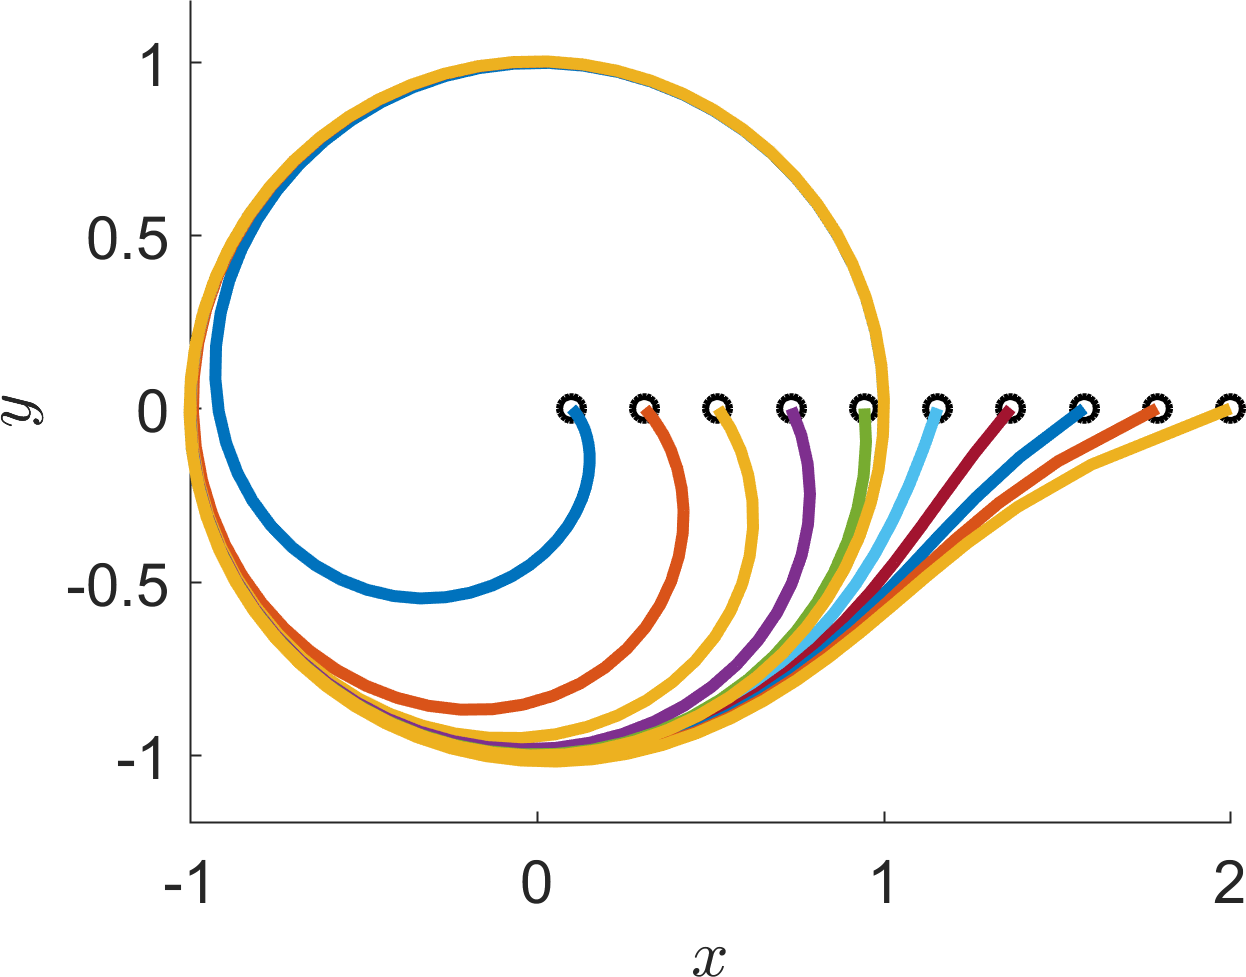
\includegraphics[width=\ttp]{../Pictures/Polar_plot.png}
\caption{\label{Polar_plot} Full dynamics of \eqns{x_polar}{y_polar}.}
\end{figure} 
\section{Check list}
By the end of this chapter you should be able to:
\begin{todolist}
\item reproduce all the definitions;
\item state all theorems;
\item solve simple linear ODE systems;
\item prove trajectories of autonomous systems cannot cross themselves;
\item prove that an ODE of one variable cannot oscillate;
\item derive single variable Taylor series of any order;
\item derive multivariate Taylor series up to first order;
\item convert systems of ODE equations of Cartesian variables in to polar variables and back again.
\end{todolist}





\chapter{How to model a system}\label{How to model a system}
\begin{aquote}{The Chemical Basis of Morphogenesis. A. Turing 1952.}
\textit{This model will be a simplification and an idealization, and consequently a falsification. It is to be hoped that the features retained for discussion are those of greatest importance in the present state of knowledge.}
\end{aquote}
\begin{aquote}{Empirical Model-Building and Response Surfaces. G. Box \& N. Draper 1987.}
\textit{All models are wrong, but some are useful.}
\end{aquote}
Modelling a system, whether it be physical, chemical, or biological, is, in some ways, more of art than a science. You try and strip away all extraneous information and mathematically describe that which is left. Sometimes there are physical laws to help you, \eg gravity, conservation of energy and mass. Other times we only have experimental intuition, \eg predator-prey interactions from population data. In either case, the central idea of modelling is that it should always form part of a cyclical process \see{Modelling_loop}.

You try to start with physical intuition (experiment), represent the important parts mathematically (model), hopefully reproduce reality (test) and, finally, use your mathematical model to predict unknown outcomes (predict). These prediction can then feed back into experiment and the process begins anew.
\begin{figure}[!!!h!!!tb]
\centering
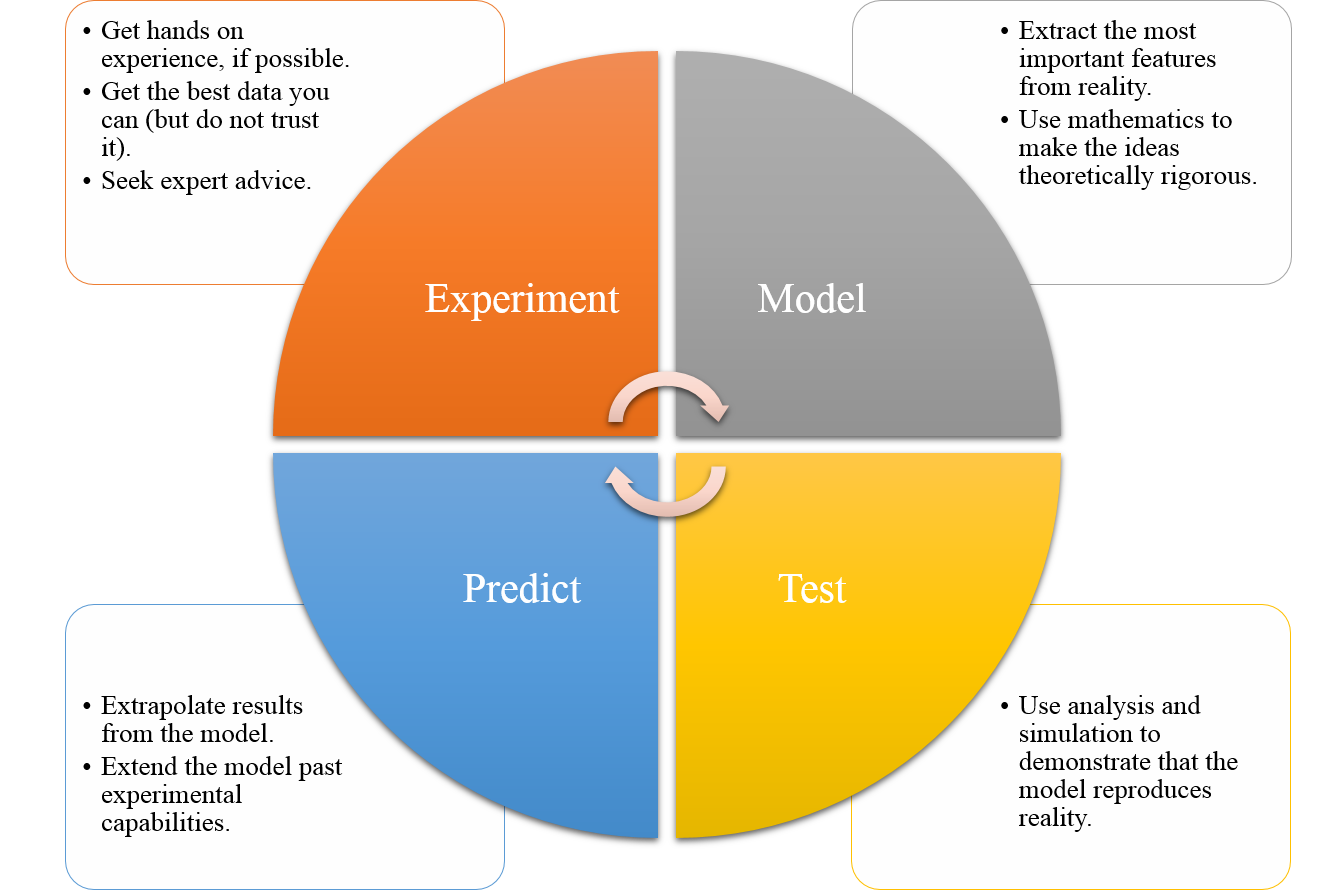
\includegraphics[width=\tp]{../Pictures/Modelling_loop.png}
\caption{\label{Modelling_loop}Diagram of the modelling cycle.}
\end{figure}

In this chapter we are going to review some of the methods that can be used to produce a mathematical interpretation of reality.

\section{Physical laws}
\begin{defin}
A \textbf{constitutive relation} (or `physical law') is a rule that the modeller adds to the system based on their experimental experience, which relates interacting components.
\end{defin}
Physics has many laws such as: conservation of energy, general relativity and the laws of thermodynamics. There is (as yet) no fundamental reason for these laws to hold. We just take them as laws because they fit the data that we observe.

Here are just a few examples of the laws that you might come across.
\begin{itemize}

\item \textbf{Newton's Law of Cooling.}

\textit{The rate of cooling of a body is proportional to the difference between the bodies temperature and the temperature of its environment.}

\COL{Let $T$ and $T_e$ be the temperatures of the object and the environment, respectively, then
\bb
\dot{T}=k(T_e-T),\label{Law_of_cooling}
\ee
where $k$ is defined to be the heat transfer coefficient.}
\begin{example}[frametitle=Cooling tea]\label{Cooling_tea}
Suppose I prepare two cups of tea at exactly the same time, so initially they both start at $100^o$C. I quickly add enough milk to cup 1 to cool it to $90^o$C. Ten minutes later I add milk to cup 2, which cools cup 2 by $10^o$C. Which cup is hotter at that point?
\COL{
The general solution to \eqn{Law_of_cooling} is
\bb
T(t)=T_e+\l T(0)-T_e\r e^{-kt},
\ee
where $T(0)$ is the initial temperature. For cup 1 we have
\bb
T_1(10)=T_{e}+\l 90-T_{e}\r e^{-k10}.
\ee
For cup 2 we have
\bb
T_2(10)=T_{e}+\l 100-T_{e}\r e^{-k10}-10.
\ee
Subtracting $T_1$ from $T_2$ gives
\bb
T_1(10)-T_2(10)=10\l 1- e^{-k10}\r>0.
\ee
Since $\exp(0)=1$ and $\exp(-kt)$ is a strictly monotonically decreasing function of time. Hence, cup 1 is hotter than cup 2 at time $t=10$ minutes. This means that the earlier you put your milk in the hotter your tea will stay!

Note that neither the ambient temperature, nor the heat transfer coefficient were needed.}
\end{example}

\item \textbf{Newton's Second Law of Motion}

\textit{The rate of change of momentum of a body is directly proportional to the force applied to the body.}

\COL{This is the standard $F=ma$ that everyone knows and loves (assuming that the mass remains that same throughout the interaction), where the acceleration, $a$, is the second derivative of the location with respect to time, $a=\ddot{x}$.}


\item \textbf{Newton's Law of Gravitation}\footnote{Newton devised the laws of optics, the laws of motion and invented calculus practically on a dare... then he turned 26. What have you done today? }

\textit{A particle attracts every other particle in the universe using a force that is directly proportional to the product of their masses and inversely proportional to the square of the distance between their centres.}

\COL{Suppose body $i$ has mass $m_i$ and is at position $\bm{r}_i=(x_i,y_i)$. Body $i$ is then separated from body $j$ by a distance $r_{ij}=\sqrt{\l x_i-x_j\r^2+\l y_i-y_j \r^2}=|\bm{r}_i-\bm{r}_j|$. Let $G$ be the universal gravitational constant then the force, $\bm{F}_{ij}$, acting on body $i$ from body $j$ is
\bb
\bm{F}_{ij}=-G\frac{m_im_j}{r^2_{ij}}\bm{\hat{r}}_{ji},
\ee
where 
\bb
\bm{\hat{r}}_{ji}=\frac{r_i-r_j}{|r_i-r_j|}
\ee
is the unit vector from body $j$ to body $i$.

Note that the force is vector valued quantity because it has a magnitude, but also a direction, as it acts in the direction of the line joining the bodies.}
\begin{figure}[!!!h!!!tb]
\centering
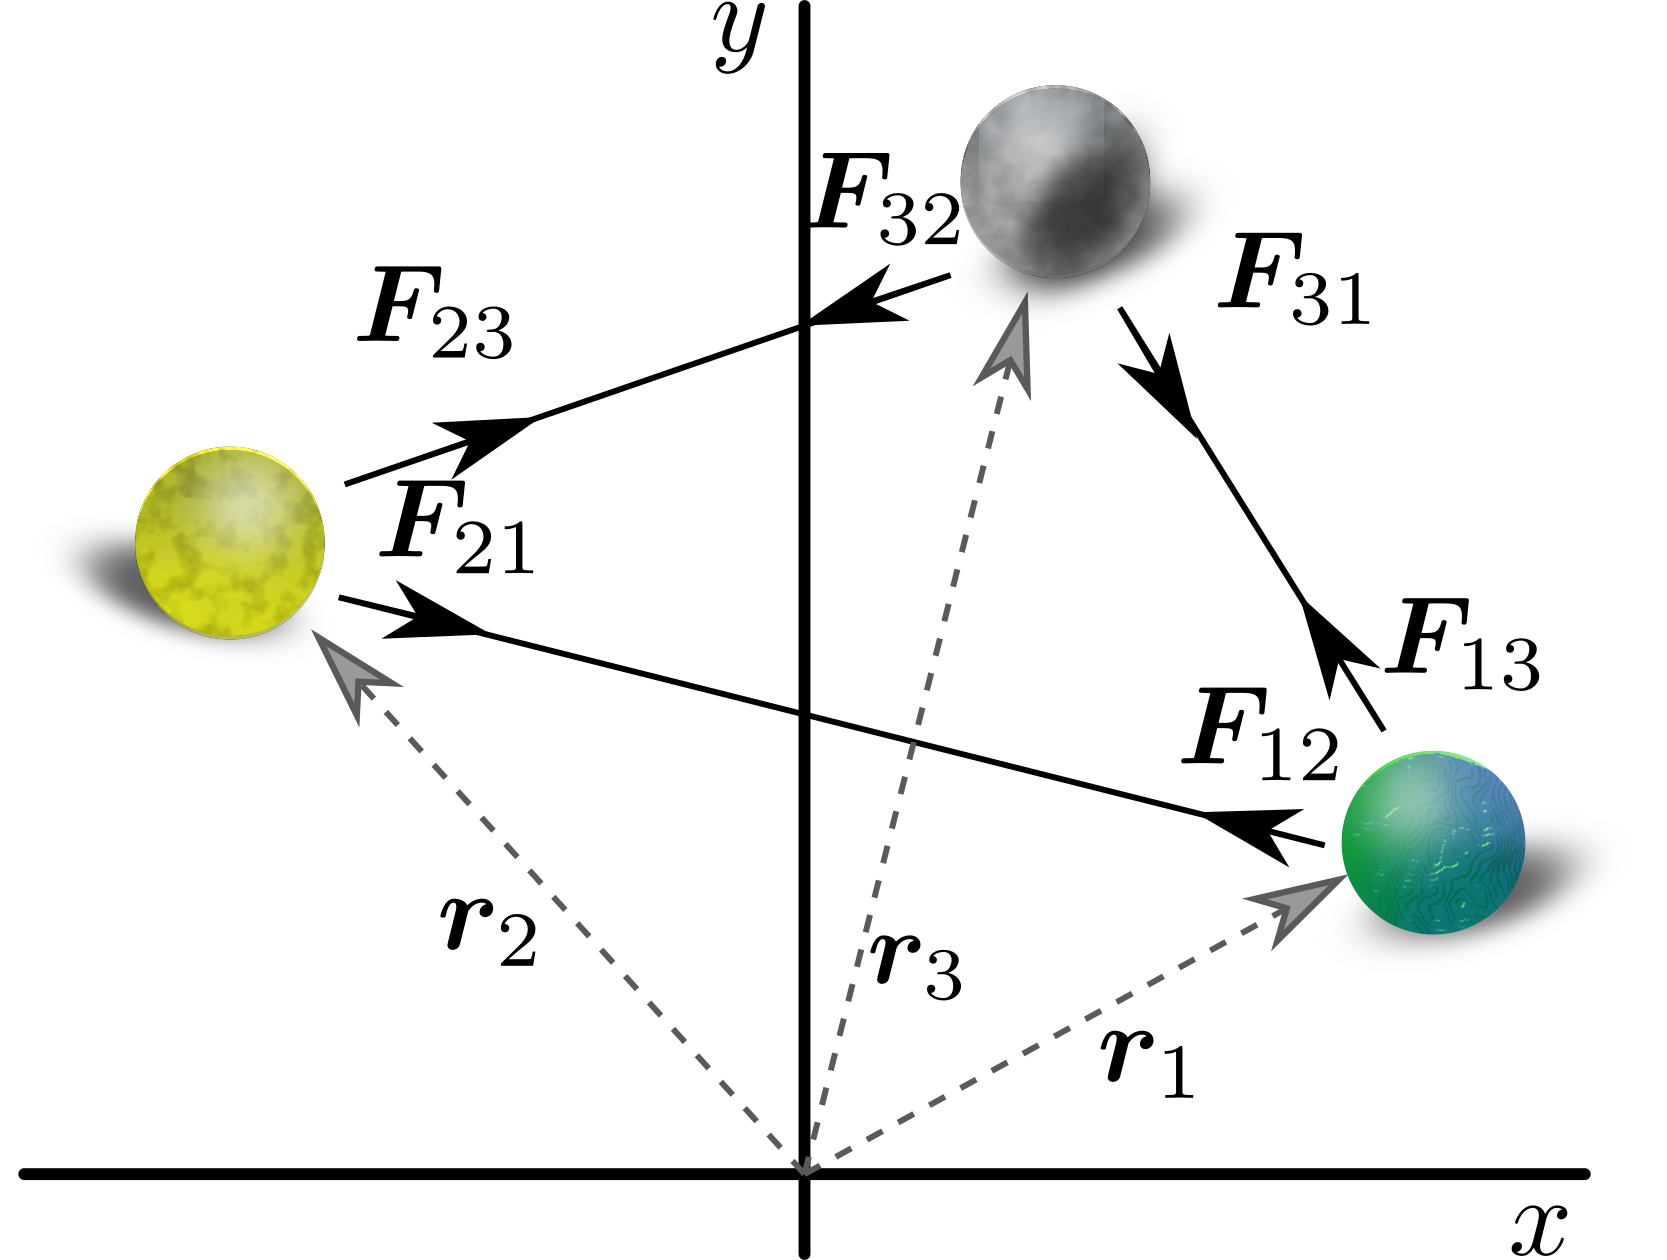
\includegraphics[width=\ttp]{../Pictures/Three_body_problem.png}
\caption{\label{Three_body}Schematic diagram of the three-body problem.}
\end{figure}


\begin{example}[frametitle=Three body problem]\label{Three_body_problem}
We can combine the Second Law of Motion and the Law of Gravitation in order to predict the position of planets interacting through their gravitational fields \see{Three_body}. Consider three planets with the same mass, $m$, and positions $\bm{r}_1(t)$, $\bm{r}_2(t)$ and $\bm{r}_3(t)$, respectively. Further, we note that since we are dealing with acceleration (a second order equation) we will need to specify two initial conditions, the position and velocity. Let the initial positions be $\bm{r}_i(0)=\bm{r}_{i0}$ and the initial velocities $\dot{\bm{r}}_i(0)=\bm{v}_{i0}$.\COL{ The governing equations are
\begin{align}
&m\ddot{\bm{r}}_1=-G\frac{m^2}{|\bm{r}_1-\bm{r}_2|^3}\l\bm{r}_1-\bm{r}_2\r-G\frac{m^2}{|\bm{r}_1-\bm{r}_3|^3}\l\bm{r}_1-\bm{r}_3\r,\label{g1}\\
&m\ddot{\bm{r}}_2=-G\frac{m^2}{|\bm{r}_2-\bm{r}_1|^3}\l\bm{r}_2-\bm{r}_1\r-G\frac{m^2}{|\bm{r}_2-\bm{r}_3|^3}\l\bm{r}_2-\bm{r}_3\r\label{g2},\\
&m\ddot{\bm{r}}_3=-G\frac{m^2}{|\bm{r}_3-\bm{r}_1|^3}\l\bm{r}_3-\bm{r}_1\r-G\frac{m^2}{|\bm{r}_3-\bm{r}_2|^3}\l\bm{r}_3-\bm{r}_2\r\label{g3}.
\end{align}
where we remember that this is a vector equation, $\bm{r}_i=(x_i,y_i)$, so there are actually six, second order ODEs here, rather than three.}

The three body problem illustrates chaotic behaviour, in the sense that the outcome is extremely sensitive to the initial conditions. This can be seen in the simulations of \fig{Three_body_sim}.

Simulation tip:
\begin{itemize}
\item when solving \eqnto{g1}{g3} numerically we could separate each equation into its Cartesian components and reduce the second order equation to two first order equations. Namely, we would introduce $(v_{ix},v_{iy})=(\dot{x}_i,\dot{y}_i)$. Thus, we would have a system of twelve ODEs to solve, with variables
\bb
(x_1,y_1,v_{1x},v_{1y},x_2,y_2,v_{2x},v_{2y},x_3,y_3,v_{3x},v_{3y}).
\ee
However, since $x_i$ and $y_i$ are perpendicular Cartesian coordinates it turns out to be a good idea to use complex numbers. Specifically, instead of writing two ODEs for each of $x_i$ and $y_i$ we can simply solve one ODE in terms of the complex quantity $\bm{r}_i=x_i+Iy_i$, which can be handled by numerical solvers. Thus, we simplify the numerical solution from twelve to six equations.
\end{itemize}
\end{example}
\begin{figure}[!!!h!!!tb]
\centering
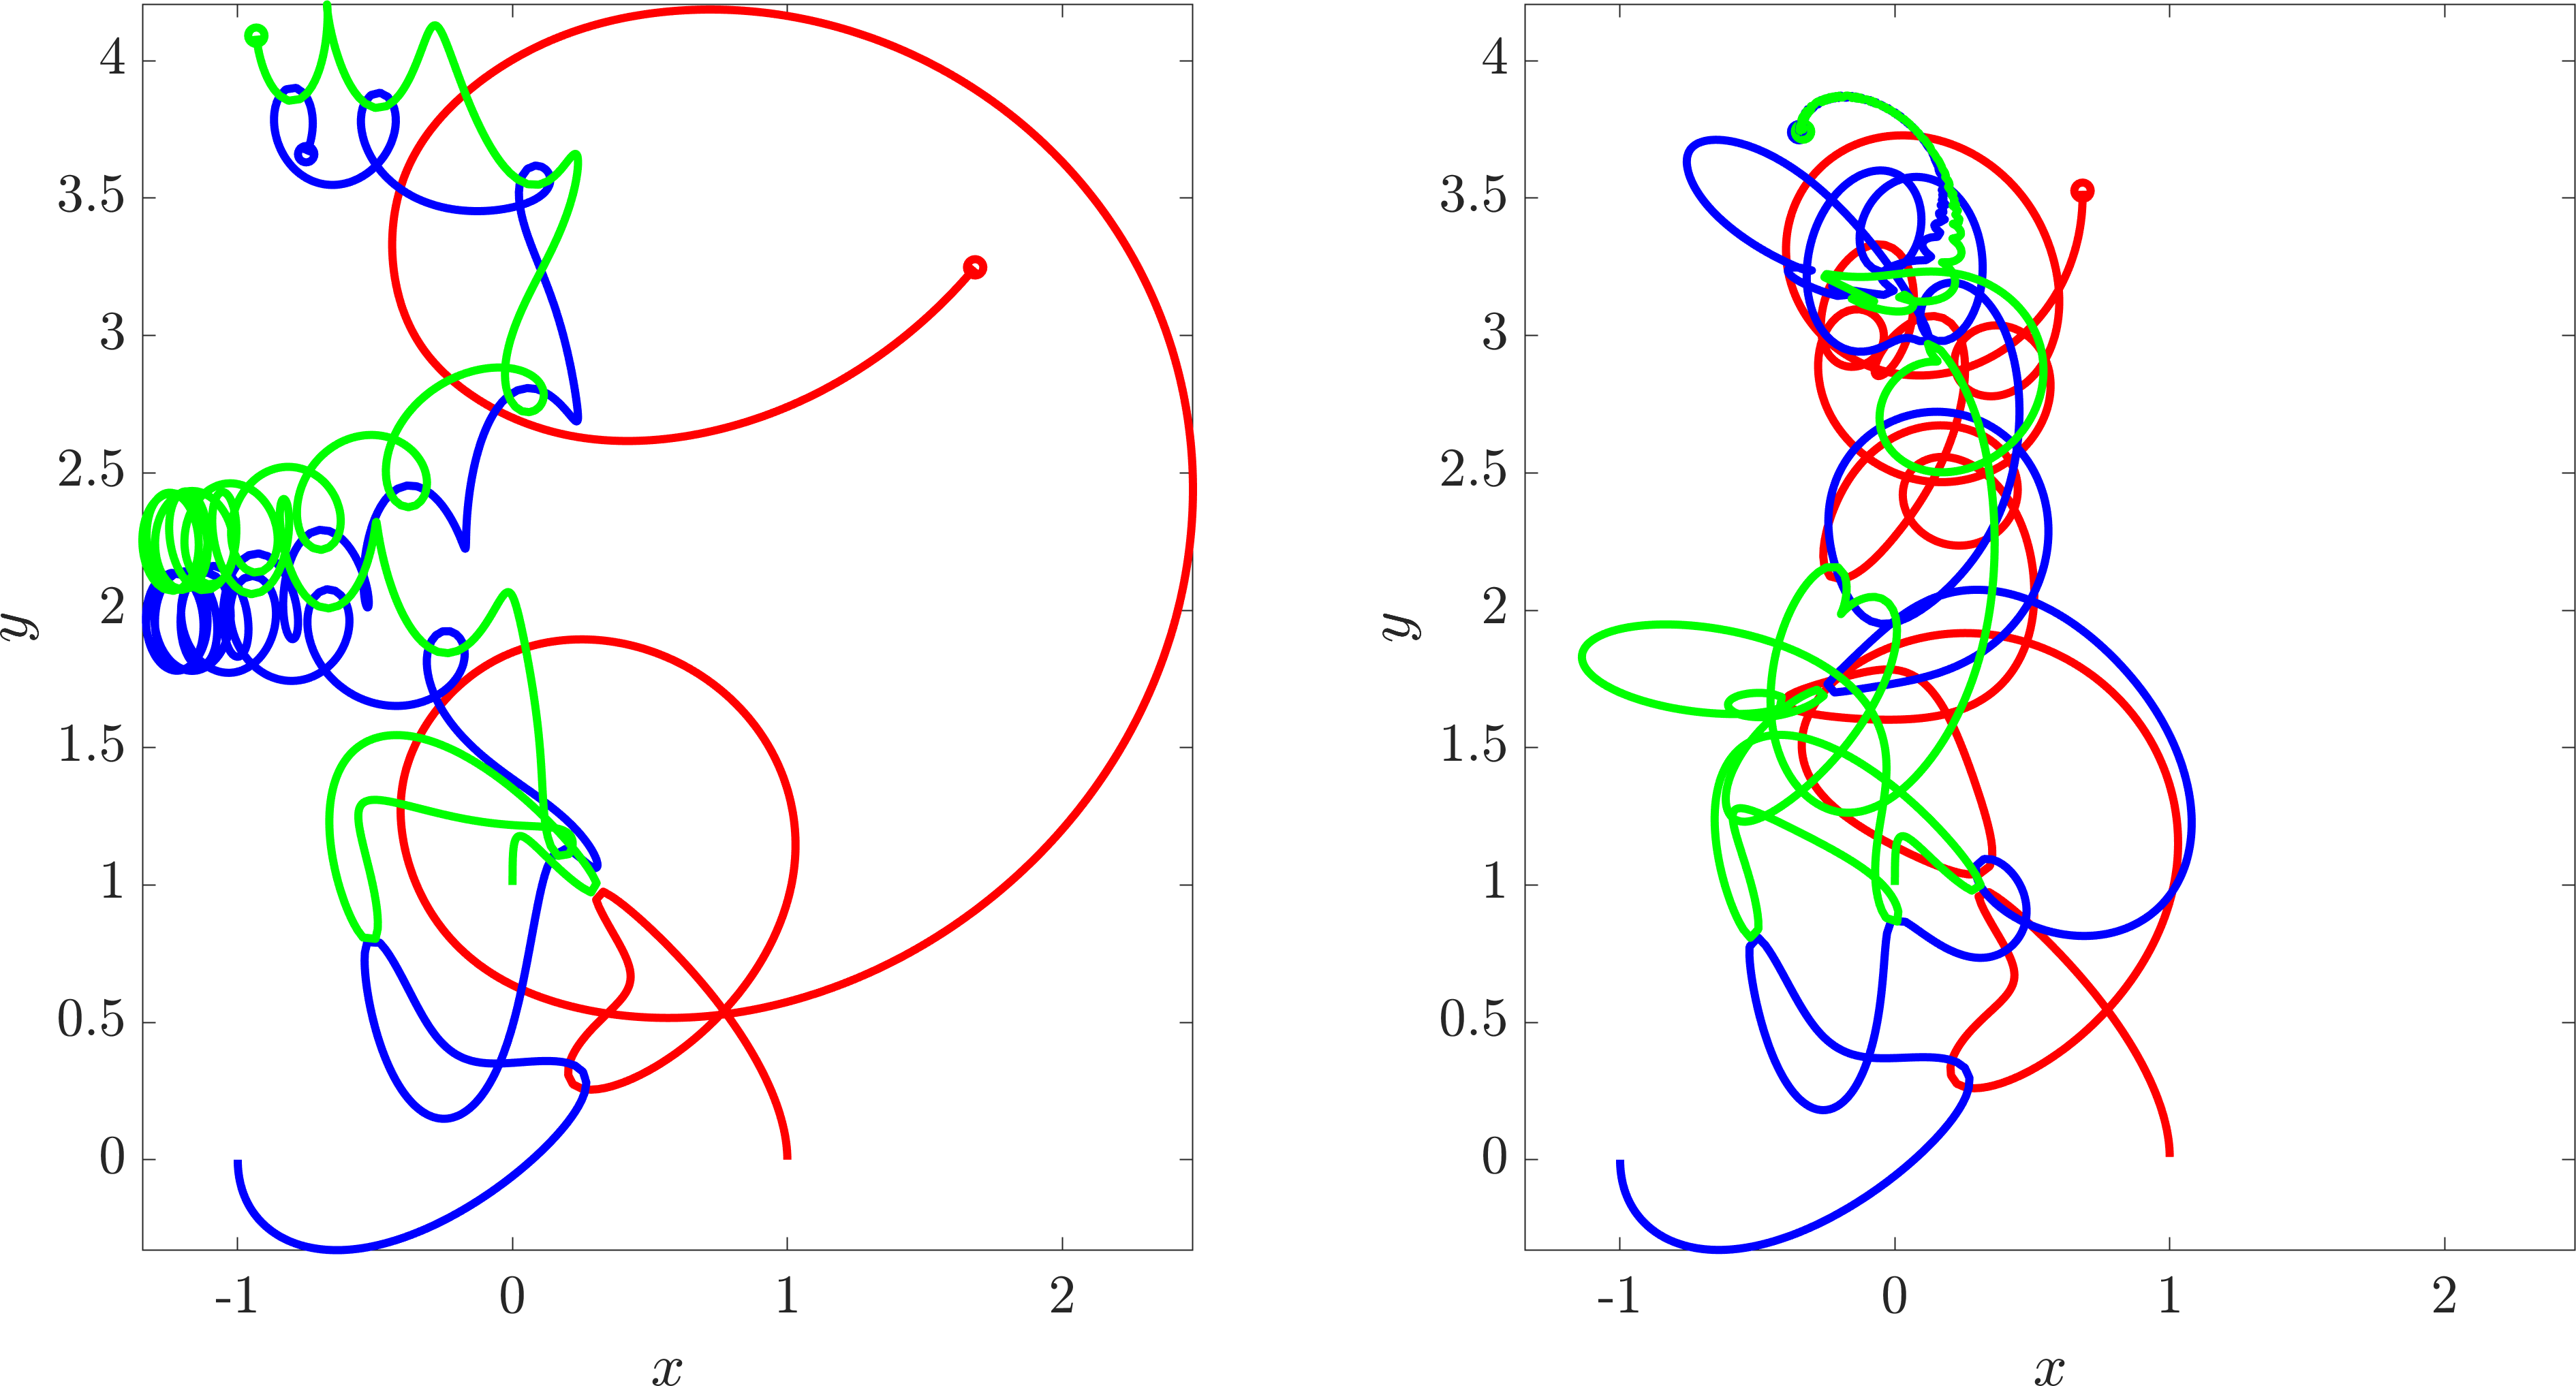
\includegraphics[width=\tp]{../Pictures/Three_body_sim.png}
\caption{\label{Three_body_sim}Two simulations of the three body problem. The green and red trajectories are identically initiated. The blue trajectory is initiated at $(-1,0.01)$ in the left figure and at $(-1,0)$ in the right figure.}
\end{figure}
\item \textbf{Hooke's law}

\textit{The force, $F$, needed to extend or compress a spring by some distance, $x$, scales linearly with respect to that distance,}
\COL{
\bb
F=kx.
\ee

The constant of proportionality, $k$, defined by this law is known as the spring constant and is measured in units of Force per distance, \eg N/m.

Depending on the material Hooke's law only holds true for small extensions and compressions. For example, this law suggests that given enough force a spring can pass through itself. Further, biological materials may not follow the law because they break if stretched too far (\eg bone), or they may grow, or permanently deform\footnote{Consider, for example, the ear. Small earrings to not stretch the skin very much and, thus, once the earring is removed the skin can heal. Alternatively, people who use large gauge earrings stretch their ear holes beyond the elastic limit of the skin so that they have a permanent hole. }, thus, reducing the force needed to give the same extension (\eg skin).
}

\end{itemize}
\subsubsection{Pendulums}\label{Pendulums_section}
In this section we take an extended look at pendulums depending on Hooke's law and simple Newtonian mechanics. Specifically, we consider a spring, oscillating up and down, and a bob, oscillating side to side \see{Pendulums}.
\begin{figure}[!!!h!!!tb]
\centering
\subfigure[\label{Spring}]{
\includegraphics[width=\ttp]{../Pictures/Spring.png}}
\subfigure[\label{Bob}]{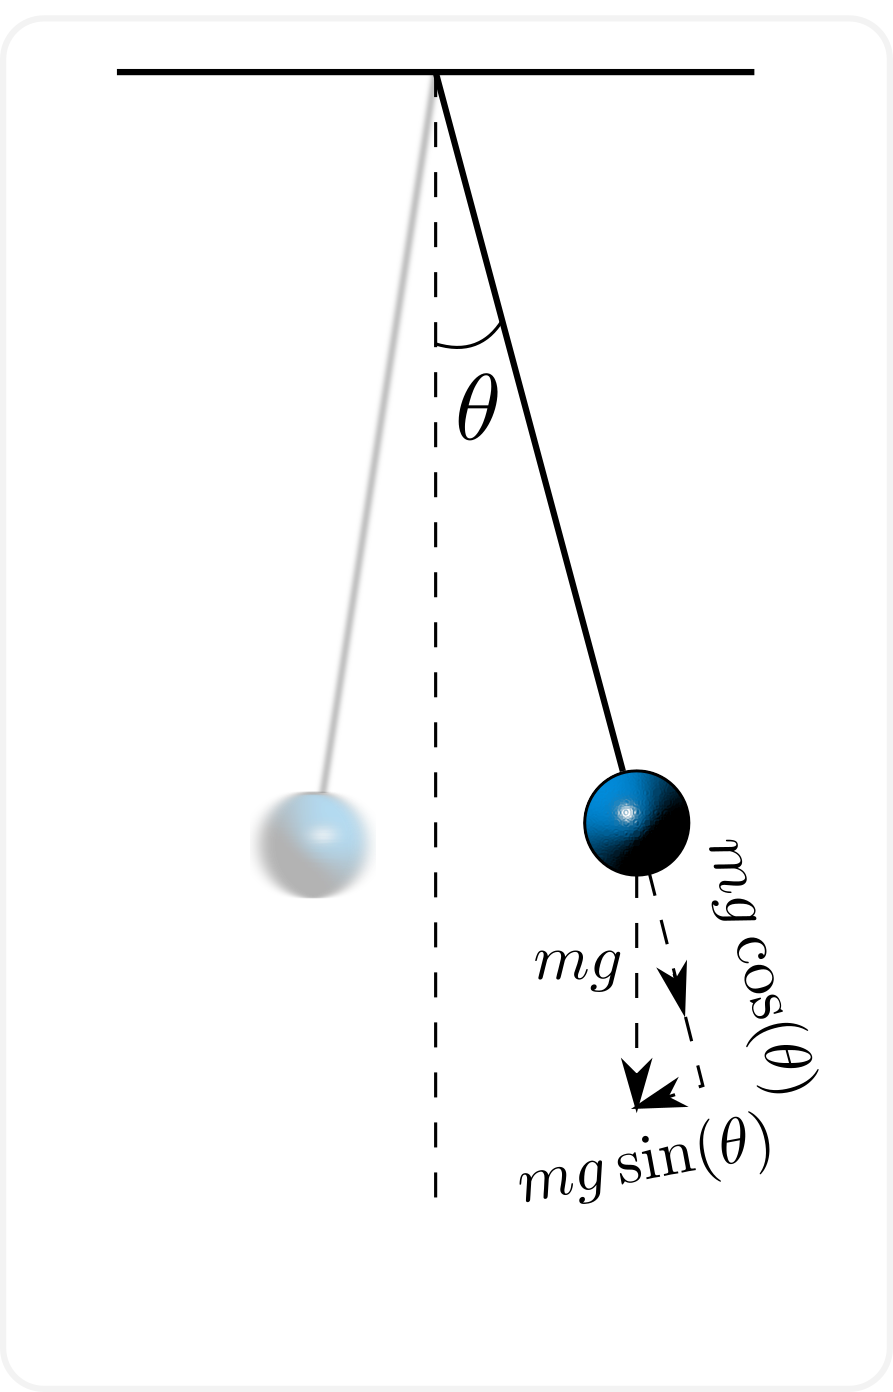
\includegraphics[width=\ttp]{../Pictures/Pendulum.png}}
\caption{Two types of pendulums: (a) an oscillating spring. (b) a weight on a string.\label{Pendulums}}
\end{figure}

\COL{Assuming that the spring conforms to Hooke's Law and applying Newton's Second Law of motion the equation of motion for the spring is
\bb
m\ddot{y}=-ky,\label{Spring_eqn}
\ee
where $y$ is the vertical displacement of the spring, $m$ is the mass attached to the spring and $k$ is the spring constant. The negative sign shows that the force is always directed to the resting position of the spring (here, taken to be the origin). If the negative sign was not there then we would be saying that the pendulums position would grow exponentially with an applied force, which is not very realistic.

The pendulum bob is slightly more complicated as we have to account for two-dimensional motion. Complicating the matter further is that the pendulum weight is confined to move on the arc of a circle, meaning that problem is easier to solve in polar coordinates.

To derive the equations of motion we split the component of force acting on the pendulum into components acting along the radial and angular directions of the system, as shown in \fig{Bob}. Critically, we only need to consider the angular acceleration, which can be derived to be $r\ddot{\theta}$. The derivation will be seen on problem sheet two. Using Newton's Second Law again we derive that
\bb
mr\ddot{\theta}=-mg\sin(\theta).\label{Bob_eqn}
\ee
One interesting point we can immediately see from \eqn{Bob_eqn} is that the mass of the pendulum does not influence the solution of the equation, which can be compared with the dependence of \eqn{Spring_eqn} on the mass. 

Equation \ref{Bob_eqn} can be solved directly in terms of `elliptic integrals', but this accounts to little more than integrating the equation twice and leaving the equation written in integral form. More insight to the solution can be gained if the angle of oscillation is small. In this case we can linearise the right-hand side of \eqn{Bob_eqn} by using Taylor series about zero, \ie $\sin(\theta)\approx\theta$. Hence, \eqn{Bob_eqn} can be approximated by
\bb
r\ddot{\theta}=-g\theta\label{Bob_eqn_approx},
\ee
which can be seen to be analogous to \eqn{Spring_eqn}.

If the different pendulums are displaced and released from rest then the amount of error introduced into the equation is determined by the initial displacement. \fig{Different_ICs} compares\footnote{Comparing $y$ and $\theta$ is a little dodgy as $y$ is a dimensional length and the $\theta$ is dimensionless, as we work in radians. However, if this bothers you we can fix this is in either of two ways. Either, we consider $y$ normalised by its natural length (taken here to be of unit length, regardless of the dimensions involved), or, we can consider \fig{Different_ICs} comparing \eqn{Bob_eqn} and its approximation in \eqn{Bob_eqn_approx}.} \eqns{Spring_eqn}{Bob_eqn} with different initial conditions. Thus, we see that increasing the initial amplitude of the bob pendulum causes the wave length of the oscillation to increase, or frequency of oscillation to decrease.}
\begin{figure}[!!!h!!!tb]
\centering
\subfigure[\label{IC_0.1}]{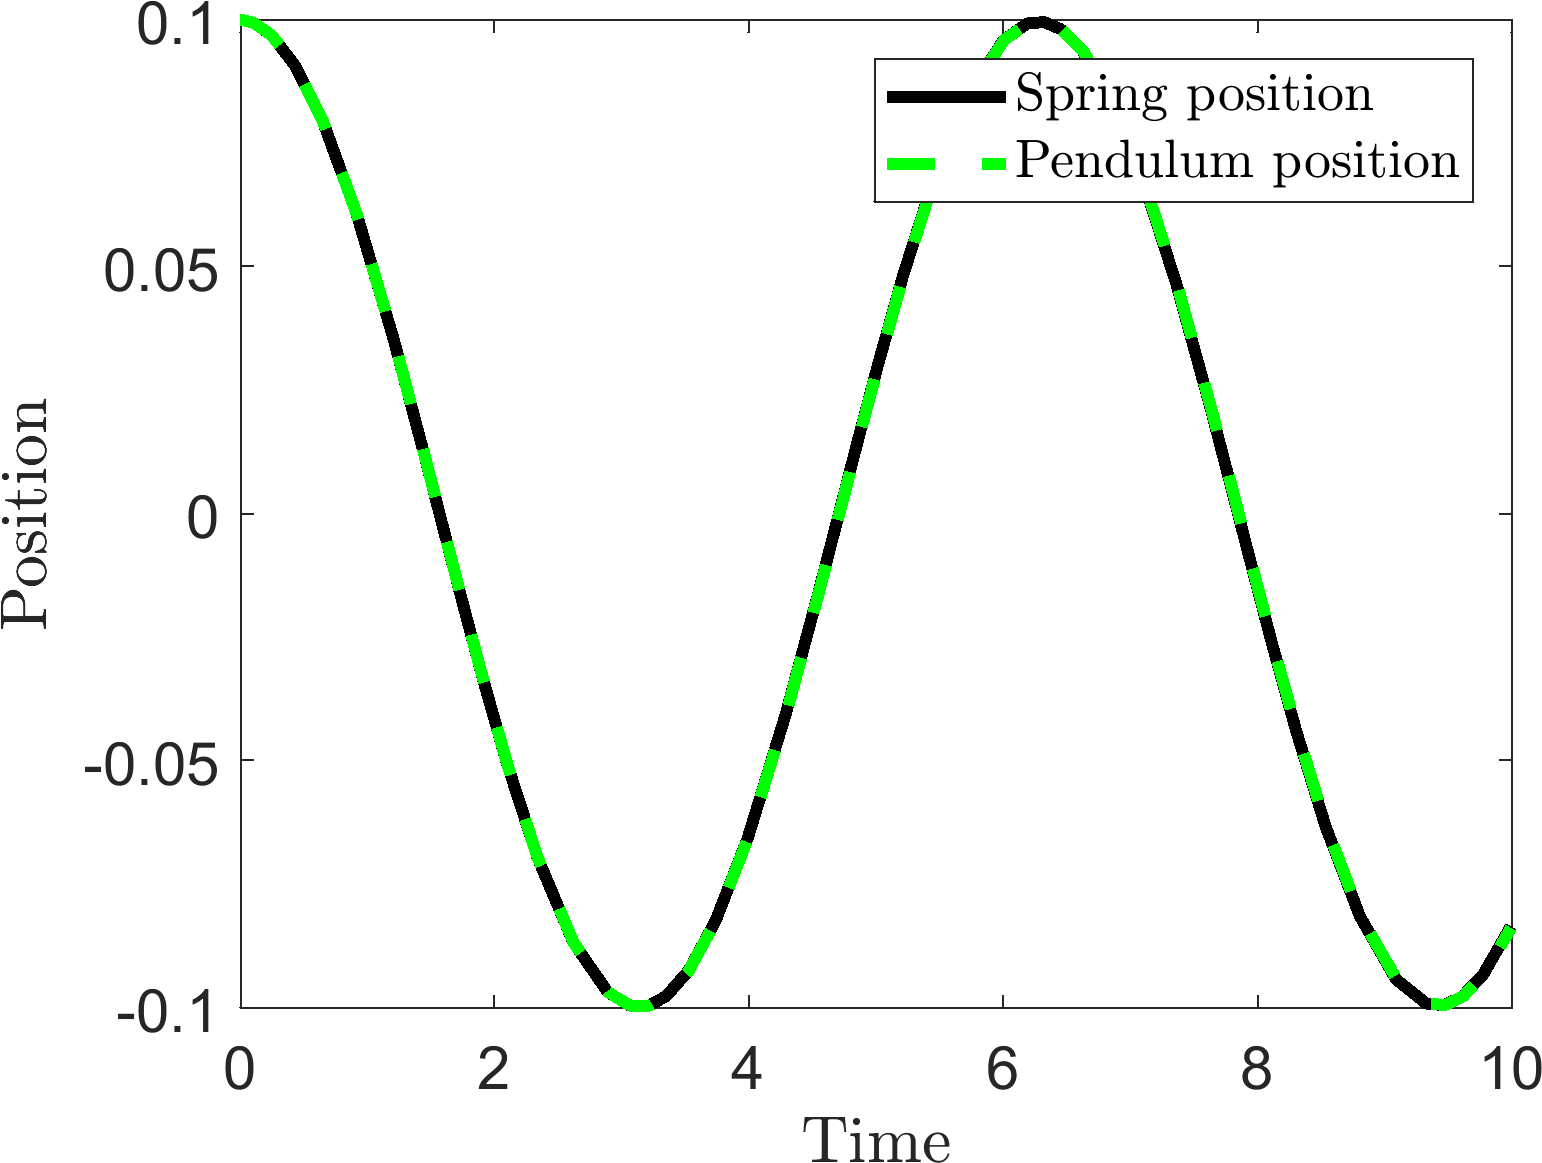
\includegraphics[width=\ttp]{../Pictures/Comparing_pendulums_IC_1.png}}
\subfigure[\label{IC_1}]{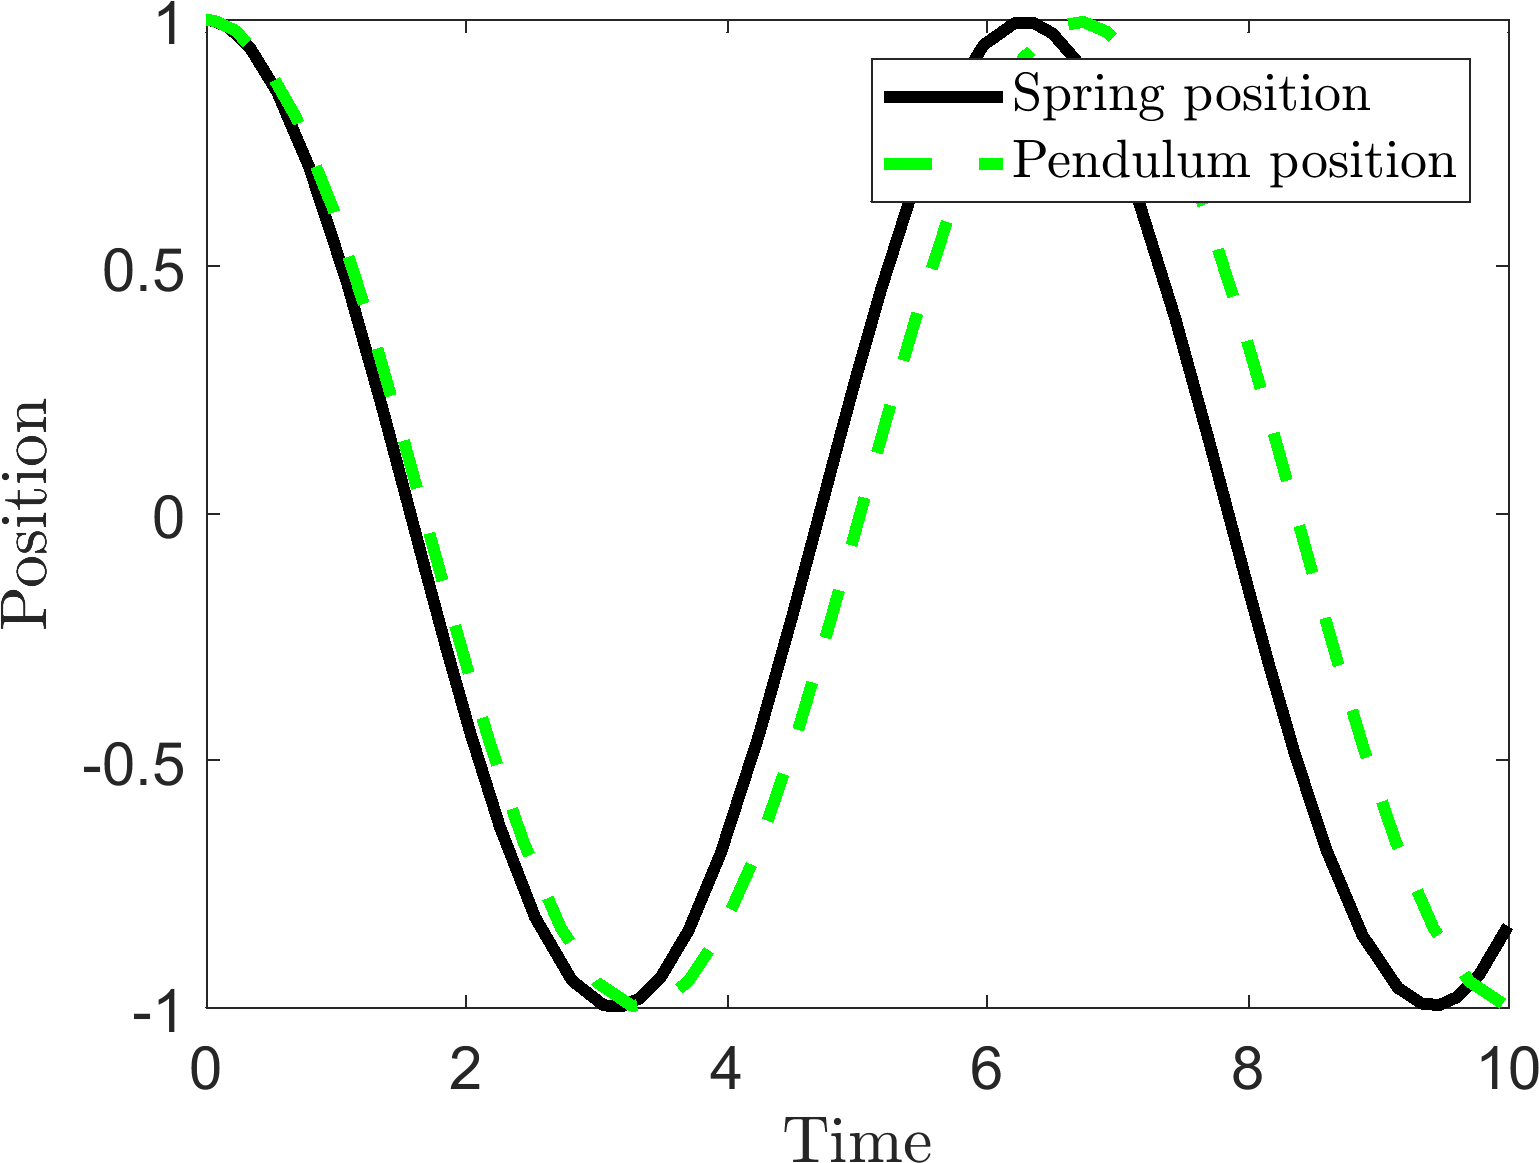
\includegraphics[width=\ttp]{../Pictures/Comparing_pendulums_IC_10.png}}
\caption{\label{Different_ICs}Comparing \eqns{Spring_eqn}{Bob_eqn} with initial conditions (a) $y=0.1=\theta$ and (b) $y=1=\theta$. Parameter values $r=g=k=m=1$.}
\end{figure}

\begin{defin}
Any system defined by an equation of the form
\bb
\ddot{u}=-k^2u.\label{SHM}
\ee
is said to under go \textbf{simple harmonic motion}.
\end{defin}
Equation \ref{SHM} can be solved to produce the solution
\bb
u=A\cos(kt)+B\sin(kt),
\ee
where $A$ and $B$ are specified through the initial conditions.

%\subsection{Euler-Bernoulli beam}
\section{Law of Mass Action}
All of the above physical laws are very specific in their application. In this section we will learn about a much more general technique that will allow us to build an ODE system out of multiple interacting populations. These populations could represent chemical compounds, humans, cells or animals as well as different states within a population \ie infected humans and susceptible humans. The law presented in this section is applied whenever the populations of the system are able to: (i) change identities; (ii) create more population members; or (iii) cause populations to decay. Specific examples of each of these interactions are, respectively: (i) susceptible humans becoming infected through interactions with a diseased person; (ii) animals giving birth; (iii) predators eating prey. Note that a change-of-identity interaction can itself be thought as a combination of creation and degradation operations. For example, in the above case of infection a member of the susceptible human population is removed from the system, whilst an infected human is added to the system. Thus, all interactions can be made through combining creation and degradation operations.

We use chemical reaction notation to specify the outcomes of population interactions. Consider a system composed of $n$ different interacting populations $(u_1,\dots,u_n)$. We assume that all interactions between the population elements lead to the creation, or destruction, of one (or more) of the $n$ populations. 
\begin{defin}
A \textbf{rate equation} specifies that an interaction involves $a_1$ members of population $u_1$, $a_2$ members of population $u_2$, etc. and produces $b_1$ members of population $u_1$, $b_2$ members of population $u_2$, etc. The equation is written as
\bb
a_1u_1+a_2u_2+\dots+a_nu_n \stackrel{r}{\rightarrow} b_1u_1+b_2u_2+\dots+b_nu_n,
\ee
where $r>0$ is the \textbf{reaction rate}.
\end{defin}
Note that some of the $a_i$ and $b_i$ values can be zero.

\begin{example}[frametitle=Reaction equation examples]\label{Reaction equation examples}
\begin{itemize}
\item \textbf{Birth}

Two agents of population $u$ come together to produce a third,
\COL{\bb
2u\stackrel{r}{\rightarrow}3u.
\ee}
\item \textbf{Death}

An agent of population $u$ dies (or is destroyed) due to natural causes,
\COL{
\bb
u\stackrel{r}{\rightarrow}\slashed{0}.
\ee}

\item \textbf{Predation}

A predator population, $v$, converts energy from eating prey, $u$, into offspring,
\COL{
\bb
u+v\stackrel{r}{\rightarrow}2v.
\ee}

\item \textbf{Infection}

Consider a population of infected people, $I$, who are able to infect a susceptible population, $S$. Further, over time, the infected people recover and become susceptible again,
\COL{\begin{align}
I+S&\stackrel{r_1}{\rightarrow}2I,\\
I&\stackrel{r_2}{\rightarrow}S.
\end{align}}
\end{itemize}
\end{example}

Rate equations provide a rigorous way of defining all of the interactions a system is assumed to undergo. However, we still require a method of converting the rate equation into an ODE. This is the power of the Law of Mass Action.
\begin{defin}
The \textbf{Law of Mass Action} states that production rate of a reaction is directly proportional to the product of the input population sizes. Specifically, if 
\bb
a_1u_1+a_2u_2+\dots+a_nu_n \stackrel{r}{\rightarrow} b_1u_1+b_2u_2+\dots+b_nu_n \nonumber
\ee
is the reaction of interest then the production rate is proportional to
\bb
ru_1^{a_1}u_2^{a_2}\dots u_n^{a_n}
\ee
and the accompanying ODEs are
\begin{align}
&\dot{u}_1=(b_1-a_1)ru_1^{a_1}u_2^{a_2}\dots u_n^{a_n},\\
&\dot{u}_2=(b_2-a_2)ru_1^{a_1}u_2^{a_2}\dots u_n^{a_n},\\
&\vdots\\
&\dot{u}_n=(b_n-a_n)ru_1^{a_1}u_2^{a_2}\dots u_n^{a_n}.
\end{align}
\end{defin}
Note that in converting from reaction equation to the ODE of $u_i$ we to account for the stoichiometry, \ie $(a_i-b_i)$. Further, when multiple reactions are considered, the terms arising from the Law of Mass Action are simply added together as independent terms.

\begin{example}[frametitle=Law of Mass Action examples]\label{Law of Mass Action examples}
\begin{itemize}
\item \textbf{Birth}
\COL{\begin{align}
2u&\stackrel{r}{\rightarrow}3u,\nonumber\\
\implies &\dot{u}=ru^2.
\end{align}}
\item \textbf{Death}
\COL{\begin{align}
u&\stackrel{r}{\rightarrow}\slashed{0},\nonumber\\
\implies &\dot{u}=-ru.
\end{align}}

\item \textbf{Predation}
\COL{\begin{align}
u+v&\stackrel{r}{\rightarrow}2v,\nonumber\\
\implies &\dot{u}=-ruv,\\
&\dot{v}=ruv.
\end{align}}

\item \textbf{Infection}
\COL{\begin{align}
I+S&\stackrel{r_1}{\rightarrow}2I,\quad I\stackrel{r_2}{\rightarrow}S,\nonumber\\
\implies &\dot{S}=-r_1IS+r_2I,\\
&\dot{I}=r_1IS-r_2I.
\end{align}}
\end{itemize}
\end{example}



\begin{example}[frametitle=Zombies]\label{Zombies}
Humans, $H$, and zombies, $Z$, interact through the following three interactions \see{Zombie_picture}:
\begin{enumerate}
\item humans kill zombies at a rate $a$;
\item zombies kill humans at a rate $b$;
\item zombies infect humans at a rate $c$.
\end{enumerate}
The reaction equations for this system are,
\COL{\begin{align}
&H+Z\stackrel{a}{\rightarrow}H;\\
&H+Z\stackrel{b}{\rightarrow}Z;\\
&H+Z\stackrel{c}{\rightarrow}2Z.
\end{align}
}\COL{The ODE form of the system is
\begin{align}
&\dot{H}=-bHZ-cHZ=-\alpha HZ\\
&\dot{Z}=-aHZ+cHZ=\beta HZ.
\end{align}
Since $\alpha=b+c>0$ the population of $H$ is always decreasing. However, $\beta=c-a$, which could be either positive or negative. Critically, if $\beta>0\implies c>a$ then the zombie population will grow. Alternatively, if $\beta<0 \implies c<a$ then  the zombie population decreases. Thus, the survival of the human race all depends on the sign of $c-a$, which, explicitly, is the `net rate increase of zombies', \ie zombie production minus zombie destruction.}
\end{example}
\begin{figure}[!!!h!!!tb]
\centering
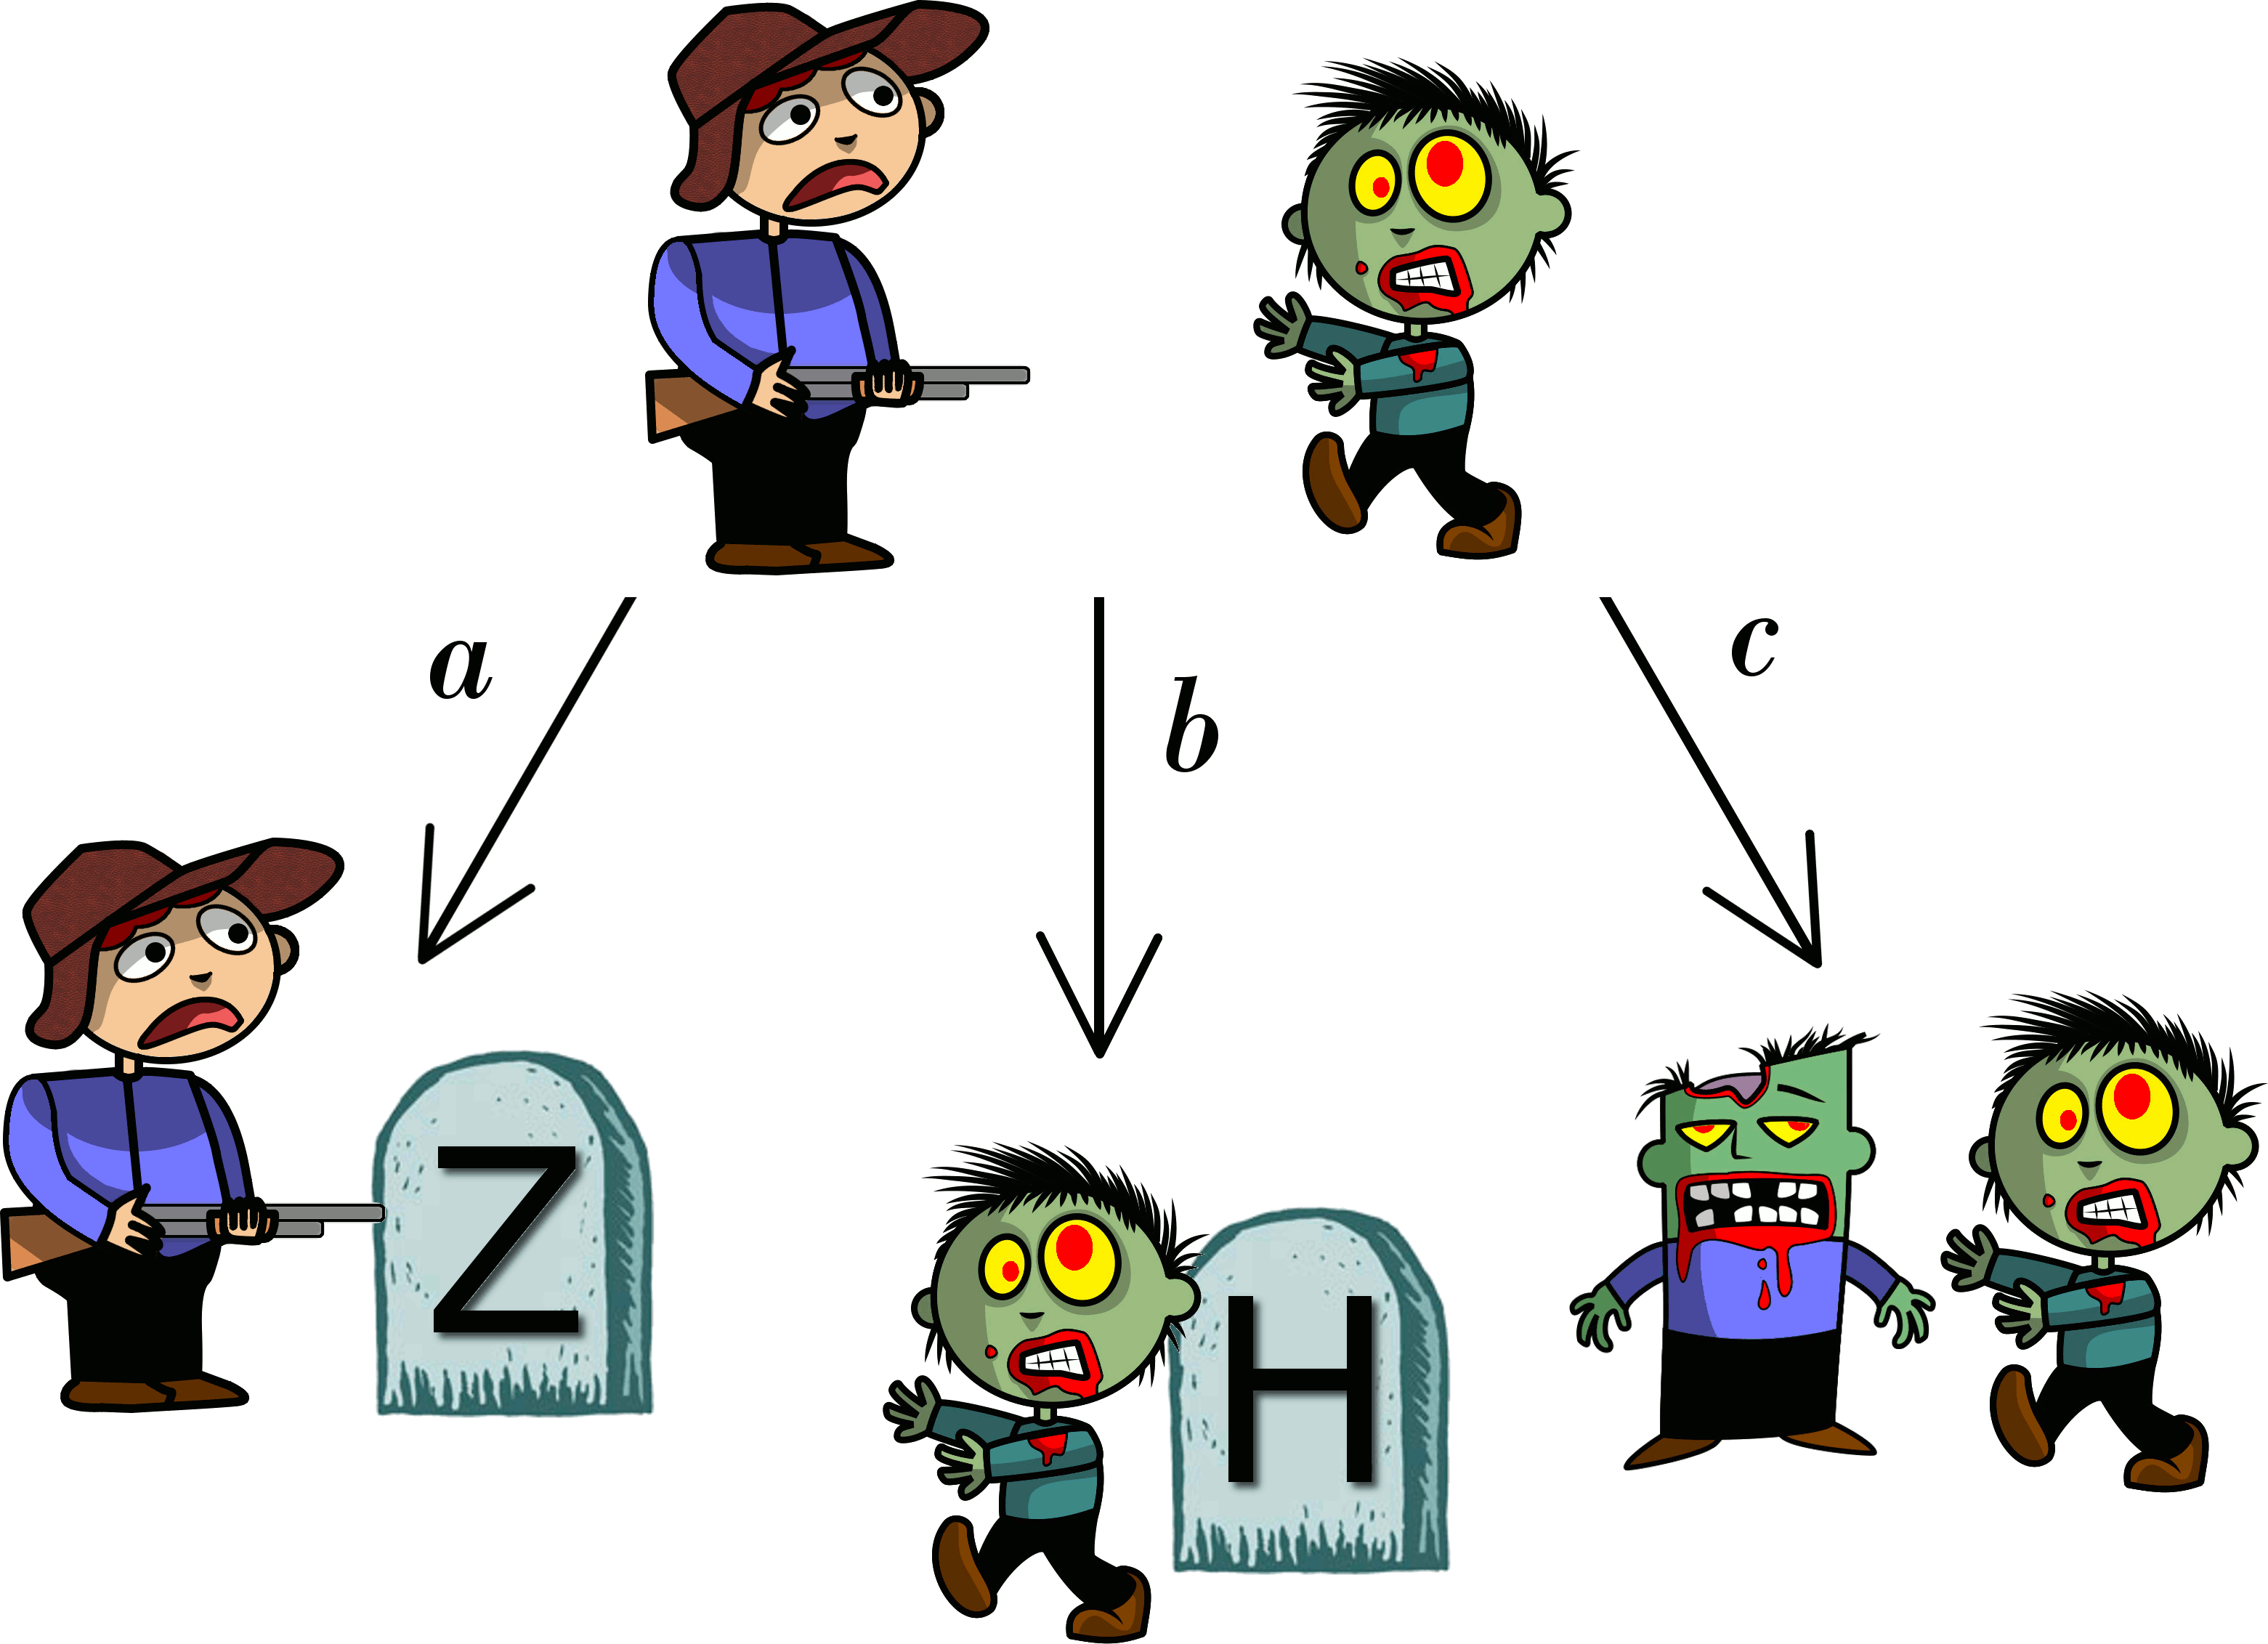
\includegraphics[width=\tp]{../Pictures/Zombies.png}
\caption{\label{Zombie_picture} Possible outcomes of human-zombie interactions.}
\end{figure}

\section{Check list}
By the end of this chapter you should be able to:
\begin{todolist}
\item define all of the constitutive laws;
\item solve problems involving Newton's laws, Hooke's law and simple harmonic motion;
\item convert a system of population interactions into reaction equations;
\item convert reaction equations into ODEs using the Law of Mass Action.
\end{todolist}





\chapter{Non-dimensionalisation}\label{Non-dimensionalisation}
\begin{aquote}{Wild Thing. J. Bazell 2013.}
\textit{In metric, one milliliter of water occupies one cubic centimeter, weighs one gram, and requires one calorie of energy to heat up by one degree centigrade — which is 1 percent of the difference between its freezing point and its boiling point. An amount of hydrogen weighing the same amount has exactly one mole of atoms in it. Whereas in the [imperial] system, the answer to ``How much energy does it take to boil a room-temperature gallon of water?" is ``Go fuck yourself'', because you can't directly relate any of those quantities.}
\end{aquote}

Thus, far we have been fairly lax about defining the quantities we have actually been measuring. Further, once we have specified what the quantity actually is, what units are we using to measure the quantity. For example, if we are measuring distance are we doing it in mm, miles or light-years? Equally, is time measured in seconds, minutes or hours? Finally, constitutive laws often introduce parameters that are not quantified accurately, or alternatively, we may be interested in understanding how a solution depends on a particular parameter as it is varied. 

The Law of Mass Action, in particular, could be thought to be a troublesome law as it introduces a rate parameter for each reaction equation that is considered. For example, if a system of ODEs is defined by a set of non-linear equations it is highly unlikely to be solvable in closed form. Thus, if there are a large number of parameters in the system, it becomes very difficult to predict how varying a single parameter (or group of parameters) will influence the solution.

However, we have already seen cases in which we do not need to consider parameters individually, as specific groups of the parameters are seen to act in the same way. For example, in the case of the spring pendulum (see \sect{Pendulums_section}), we saw that the frequency of oscillation depended on $\sqrt{k/m}$. Thus, stiffening the spring (increasing $k$) has the same effect on the solution as decreasing the mass (decreasing $m$), \ie they both increase the frequency of the oscillations. Equally, in the example of a zombie infection (see example \ref{Zombies}), the parameters of interest were not $a$, $b$ or $c$, but rather $\alpha=b+c$ and $\beta=c-a$.

In this chapter we introduce a technique, called non-dimensionalisation, that will benefit us in two ways. Firstly, it allow us to brush away worries about dealing with units and, secondly, it will allow us to reduce the number of effective parameters in our system. Specifically, we will be able to define parameter groupings that will influence the final result in the same way.

\section{The central idea}
To non-dimensionalise a system of equations, we have the following rules:
\begin{enumerate}
\item Identify all the variables;
\item Replace each variable with a quantity scaled relative to a characteristic unit of measure (to be determined);
\item Choose the definition of the characteristic unit for each variable;\label{Choose}
\item Rewrite the system of equations in terms of the new dimensionless quantities.
\end{enumerate}
We note three particular points about these rules. Firstly, the theory behind non-dimensionalisation is straight forward. Namely, we substitute scaled variables into an equation system and massage the equations until we have rearranged the system to produce the desired outcome. However, in practice the difficulty of the technique lies in the algebraic manipulation; it is very easy for the terms to become lost during the manipulation. Thus, care must be taken during the algebraic manipulation stage.

Secondly, you will notice the word `choose' in point \ref{Choose}. This means that it possible to construct many different non-dimensionalised systems from the same system of equations, \ie non-dimensionalisation is non-unique. We usually choose the characteristic unit of each variable to either emphasise one of the terms in a system or to remove as many parameters as possible.

Finally, this technique is hard to demonstrate in generality. It is much better to consider a number of system and see how the technique works in action. Thus, what follows will be a select number of examples, which along with your problem sheets should give you a good basis in the theory. However, do not think that these are all the examples you could face.

It should be noted that there is little consistency in nomenclature across book when considering the separation of variables into their dimensional and non-dimensional components. Thus, always be clear in your definitions.

\subsection{Examples of non-dimensionalisation through substitution of variables}\label{Examples of non-dimensionalisation through substitution of variables}
\begin{example}[frametitle=Substituting variables]
\begin{itemize}
\item Consider the equation for exponential growth,
\bb
\dot{u}=ru, \quad u(0)=u_0.\label{Non-dim_1}
\ee
\COL{The variables in \eqn{Non-dim_1} are $u$ and $t$. We rewrite them as $u=[u]u'$ and $t=[t]t'$, where $[u]$ and $[t]$ are the dimensional scales and $u'$ and $t'$ are the non-dimensional variables. We are free to define the values of $[u]$ and $[t]$ as we please. It is our job to choose appropriate definitions that simplify \eqn{Non-dim_1}. Critically, although we are free to choose the value of $[u]$ and $[t]$ the values must have consistent units. Namely, $[t]$ must have units of time and $[u]$ must have units of density.

We substitute the expanded variables into \eqn{Non-dim_1} and rearrange to produce
\bb
\frac{\rd u'}{\rd t'}=[t]ru', \quad u(0)=\frac{u_0}{[u]}.\nonumber
\ee
Hence, we see that if we choose $[t]=1/r$ and $[u]=u_0$ then \eqn{Non-dim_1} simplifies to
\bb
\dot{u}=u, \quad u(0)=1,\nonumber
\ee
where we note that we have dropped the prime symbols, $'$, for notational convenience.

For mathematicians dropping primes is often done as the last step because we infrequently care about the actual values of the variables, rather we study the dynamics available in the equation. However, in any specific application we should be careful to remember that the variables we are dealing with are non-dimensional and that the solution is not complete until we `re-dimensionalise' the variables.}

\COL{In this example we see that the values of $r$ and $u_0$ in \eqn{Non-dim_1} do not influence the dynamics of the simulation. Specifically, they only scale the time and initial condition.

Although this was a fairly trivial example, a good way to check consistency of the answer at the end of the manipulation is to check that all of the dimensions agree. As mentioned $[t]$ should have units of time and $[u]$ should have units of density. We return to \eqn{Non-dim_1} and consider the dimensions of each component.

For example, $\dot{u}=\rd u/ \rd t$ has units of density/time. By equality, $ru$ must have units of density/time since $u$ has units of density then $r$ must have units of 1/time. Thus, 
\bb
\textrm{dim}([t])=\textrm{dim}(1/r)=\textrm{time}.\nonumber
\ee
Equally, $[u]=u_0$ can trivially be seen to have the correct units of density.}

\item Consider the equation for logistic growth,
\bb
\dot{u}=ru\l 1-\frac{u}{K} \r, \quad u(0)=u_0.\label{Non-dim_2}
\ee
\COL{Again, $u=[u]u'$ and $t= [t]t'$ can be substituted into \eqn{Non-dim_2} to produce
\bb
\frac{\rd u'}{\rd t'}=[t]ru'\l 1-\frac{[u]}{K}u'\r,\quad u'(0)=\frac{u_0}{[u]},\nonumber
\ee
from which we see that it would be wise to once again take $[t]=1/r$. Beyond this we see that we have a choice. Should we take $[u]=K$, or $[u]=u_0$? Both are valid non-dimensionalisations and either maybe be appropriate depending on the context of the problem. 

Here, we are going to take $[u]=K$ as we are interested in the dynamics of the system, rather than the initial condition. Thus, after dropping primes we see that we can non-dimensionalise \eqn{Non-dim_2} to 
\bb
\frac{\rd u}{\rd t}=u\l 1-u\r,\quad u(0)=U_0,\nonumber
\ee
where $U_0=u_0/[u]=u_0/K$.

In this case the non-dimensionalisation demonstrates that the only parameter that the solution depends on is the initial conditions. Changing $r$ does not change the dynamics of the system, it only changes the time scale, since $r=1/[t]$. Equally, changing $K$ simply scales the size of the solution, as $u=Ku'$.}

\item Consider the following equations (the Schnakenberg kinetics)
\begin{align}
&\dot{u}=k_1-k_2u+k_3u^2v, \quad u(0)=u_0,\label{Non-dim_31}\\
&\dot{v}=k_4-k_3u^2v, \quad v(0)=v_0.\label{Non-dim_32}
\end{align}
\COL{This time we use the scales $u=[u]u'$, $v=[v]v'$, $t=[t]t'$ to derive
\begin{align}
&\frac{\rd u'}{\rd t'}=\frac{[t]k_1}{[u]}-[t]k_2u'+[t]k_3[u][v]u'^2v', \quad u'(0)=\frac{u_0}{[u]},\nonumber\\
&\frac{\rd v'}{\rd t'}=\frac{[t]k_4}{[v]}-[t]k_3[u]^2u'^2v', \quad v'(0)=\frac{v_0}{[v]}.\nonumber
\end{align}}\COL{
Lots of potential choices for scale balances; how do we choose? In an exam you will be given the form of an equation to produce and your task will be to derive the corresponding scales. For example, suppose we wanted to convert \eqns{Non-dim_31}{Non-dim_32} into
\begin{align}
&\frac{\rd u'}{\rd t'}=\alpha-u'+u'^2v', \quad u'(0)=u'_0\nonumber\\
&\frac{\rd v'}{\rd t'}=\beta-u'^2v', \quad v'(0)=v'_0,\nonumber
\end{align}
then we know that we would have to set
\bb
1=[t]k_3[u][v]=[t]k_2=[t]k_3[u]^2.\nonumber
\ee
Thus,
\begin{align}
&[t]=\frac{1}{k_2},\nonumber\\
&[u]=\sqrt{\frac{1}{[t]k_3}}=\sqrt{\frac{k_2}{k_3}},\nonumber\\
&[v]=[u]=\sqrt{\frac{k_2}{k_3}},\nonumber
\end{align}
which means that
\begin{align}
\alpha=\frac{[t]k_1}{[u]}=\frac{k_1}{k_2}\sqrt{\frac{k_3}{k_2}},\nonumber\\
\beta=\frac{[t]k_4}{[v]}=\frac{k_4}{k_2}\sqrt{\frac{k_3}{k_2}},\nonumber\\
u'_0=\frac{u_0}{[u]}=u_0\sqrt{\frac{k_3}{k_2}},\nonumber\\
v'_0=\frac{v_0}{[v]}=v_0\sqrt{\frac{k_3}{k_2}}.\nonumber
\end{align}

Finally, we check the consistency of the scales. From \eqns{Non-dim_31}{Non-dim_32} we infer that
\bb
\textrm{dim}(k_1)=\frac{\textrm{density}}{\textrm{time}}, \quad \textrm{dim}(k_2)=\frac{1}{\textrm{time}}, \quad \textrm{dim}(k_3)=\frac{1}{\textrm{density}^2\textrm{time}}, \quad \textrm{dim}(k_4)=\frac{\textrm{density}}{\textrm{time}}.\nonumber
\ee
Hence,
\bb
\textrm{dim}([u])=\sqrt{\frac{1/\textrm{time}}{1/(\textrm{density}^2\textrm{time})}}=\sqrt{\textrm{density}^2}=\textrm{density}.
\ee
The scales $[v]$ and $[t]$ can be checked similarly. We also need to ensure the the variables $\alpha, \beta, u'_0, v'_0$ are have no dimension. For example
\bb
\textrm{dim}(v'_0)=\textrm{density}\sqrt{\frac{1/(\textrm{density}^2\textrm{time})}{1/\textrm{time}}}=\textrm{density}\sqrt{\frac{1}{\textrm{density}^2}}=1.
\ee
The other variables can be checked similarly.}
\end{itemize}
\end{example}

\subsection{Examples of non-dimensionalisation through the arrow method}
The substitution method shown in \sect{Examples of non-dimensionalisation through substitution of variables} will always work supposing that the algebra is manipulated correctly. However, the method can be cumbersome and slow. Moreover, because it involves lots of algebraic manipulations there are many chances to make a mistake.

An alternative method rests on using arrows to identify the desired balances. This can be much quicker as the initial stages do not require laborious substitution. However, we have to be more careful because not all balances that we can `draw' using the arrows will be valid.

The idea behind the arrow method is that you draw arrows between the quantities that are going to `balance', which simply means they are going to have the same coefficient in the final non-dimensionalised form. The process is generally the same as the substitution method. However, we must remember that in order to specify the problem completely the number of valid arrow balances must equal the number of variables. For example, if a problem depends on $u$ and $t$ we would need two balances. Alternatively, if the problem depended on $u$, $v$, and $t$ we would need three valid balances.  This section is going to depend primarily on examples, again, and we will see an invalid balance at the end of the demonstrations.
\begin{example}[frametitle=Arrow method]\label{Arrow method}
\item Consider the following equation
\bb
  \tikzmark{a}\dot{u}=k_0+k_1\tikzmark{b}u+k_2\tikzmark{c}u^2, \quad u(0)=u_0.\label{Non-dim_4}
\tikz[overlay,remember picture]
{\draw[square arrow1] (a.south) to (b.south);}
\tikz[overlay,remember picture]
{\draw[square arrow1] (b.south) to (c.south);}
\ee
\COL{We have two variables, $u$ and $t$, and so we need two balances. Specifically, the arrows state that we want to balance the derivative, linear and quadratic terms,
\bb
\frac{[u]}{[t]}=k_1[u]=k_2[u]^2,\nonumber
\ee
from which it is simple to discover that
\bb
[t]=\frac{1}{k_1},\quad [u]=\frac{k_1}{k_2}.\nonumber
\ee
We still need to substitute the scales into the equations. Namely, $u=u'k_1/k_2$ and $t=t'/k_1$, but again the arrow method simplifies this task. Specifically, we know that, by design, the coefficient of the derivative, linear and quadratic term are going to be the same. Thus, we can divide through by one of them to speed up the derivation,
\bb
\frac{\rd u'}{\rd t'}=\frac{k_0}{k_1[u]}+u'+u'^2.\nonumber
\ee
Finally, redefining the last parameter as $\alpha=k_0/(k_1[u])=k_0k_2/(k_1^2)$ and the initial condition $u'(0)=k_2u_0/k_1=u'_0$, we can non-dimensionalise \eqn{Non-dim_4} to the final form of
\bb
\dot{u}=\alpha+u+u^2,\quad u(0)=u'_0,\label{Non-dim_5}
\ee
where we have dropped the primes from the variables for simplicity. Once again, we would have to ensure that $\alpha$ and $u'_0$ where non-dimensional and that $[u]$ and $[t]$ had the right dimensions, but this }\COL{is left as an exercise.
}\COL{
In this example we can illustrate the power of the non-dimensionalisation through the parameter groupings
\bb
\alpha=\frac{k_0k_2}{k_1^2},\quad u'_0=\frac{k_2u_0}{k_1}.\nonumber
\ee
Specifically, suppose we double each of the kinetic parameters \ie $k_0\mapsto 2k_0$, $k_1\mapsto 2k_1$ and $k_2\mapsto 2k_2$ then neither $\alpha$, nor $u'_0$ changes. This means that under this transformation the solution of \eqn{Non-dim_5} is exactly the same. But, how does this transformation of the original equations? Well, $[u]=k_1/k_2$ does not change, but $[t]=1/(2k_1)$ will be half its previous value. Hence, the solution to this `doubled-parameter' problem (call it $u_2(t)$) will reach the same solution values as the original problem, but in half the time \see{Non_dim_example},
\bb
u_2(t)=u\l\frac{t}{2}\r.\label{Non-dim_6}
\ee}

% we notice that if we double the value of $k_2$ and simultaneously half $k_0$ and $u_0$ then the values of $\alpha$ and $u'_0$ do not change, this means that the solution of \eqn{Non-dim_5} is the same under this transformation and, thus, so must the solutions of \eqn{Non-dim_4}.
\end{example}
\begin{figure}[!!!h!!!tb]
\centering
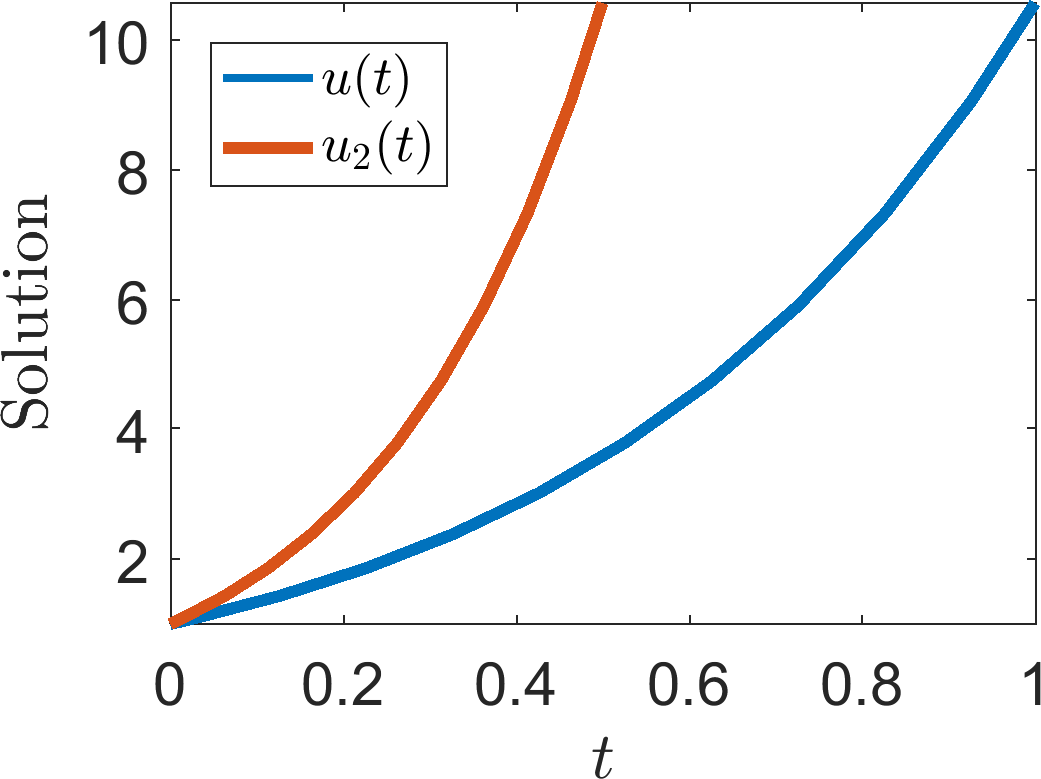
\includegraphics[width=\ttp]{../Pictures/Non_dim_example.png}
\caption{\label{Non_dim_example} Two simulations of \eqn{Non-dim_4} with parameter values $k_0=k_1=k_2=1$ (blue line, $u(t)$) and $k_0=k_1=k_2=2$ (red line, $u_2(t)$). Illustrating that the evolution of the red line is the same as the blue line, except that the red line evolution occurs twice as fast, as predicted by \eqn{Non-dim_6}.}
\end{figure}

\begin{example}[frametitle=Non-uniqueness]
 To illustrate the non-uniqueness of non-dimensionalisation we rerun example \ref{Arrow method} but this time we balance the time derivative, the constant term and the initial condition,
\bb
  \tikzmark{a}\dot{u}=k_0\tikzmark{b}+k_1u+k_2u^2, \quad u\tikzmark{c}(0)=u_0\tikzmark{d}.\label{Non-dim_7}
\tikz[overlay,remember picture]
{\draw[square arrow1] (a.south) to (b.south);}
\tikz[overlay,remember picture]
{\draw[square arrow1] (c.south) to (d.south);}
\ee
\COL{We quickly find that
\bb
\frac{[u]}{[t]}=k_0,\quad [u]=u_0,\nonumber
\ee
thus, $[t]=u_0/k_0$. We can divide the equation through by $k_0$, because we know that this is the }\COL{balance of the first two terms in \eqn{Non-dim_7}. Thus, we derive
\bb
\dot{u'}=1+\frac{k_1[u]}{k_0}u'+\frac{k_2[u]^2}{k_0}u'^2, \quad u'(0)=1,\nonumber
\ee
which would be rewritten as
\bb
\dot{u}=1+\beta u+\gamma u^2, \quad u(0)=1,\label{Non-dim_8}
\ee
where
\bb
\beta=\frac{k_1u_0}{k_0},\quad \gamma=\frac{k_2u_0^2}{k_0}.\nonumber
\ee}
\end{example}

Both forms of the non-dimensionalised equation, \eqref{Non-dim_5} and  \eqref{Non-dim_8}, are perfectly valid. The most useful form will depend on what factor dominates the equation. If $k_0$ is small and $k_1$ is big (relative to one another) then \eqn{Non-dim_5} would be more useful as $\alpha\approx0$ and we would be able to manipulate the equation to provide more information. Alternatively, if $k_0$ was big and $k_2$, or $k_1$, was small then, \eqn{Non-dim_8} would be more useful as we would, again, be able to remove one of the constants based on this assumption.

\begin{example}[frametitle=Failure]
As mentioned not all balances are valid, which is what we will be seen in this example. Consider the following ODE system
\begin{align}
  \tikzmark{a}\dot{u}=k_0\tikzmark{b}+k_1\tikzmark{c}u-k_2uv, \quad u(0)=u_0,\\
 \nonumber \\
    \tikzmark{e}\dot{v}=k_3\tikzmark{f}+k_4\tikzmark{g}v-k_2uv, \quad v(0)=v_0.
\tikz[overlay,remember picture]
{\draw[square arrow1] (a.south) to (b.south);}
\tikz[overlay,remember picture]
{\draw[square arrow1] (b.south) to (c.south);}
\tikz[overlay,remember picture]
{\draw[square arrow1] (e.south) to (g.south);}
\end{align}
\COL{There are three variables $u$, $v$ and $t$ and so we need three balances. The chosen balances are illustrated on the equations using arrows. Extracting information from the balances we find that
\bb
\frac{[u]}{[t]}=k_0=k_1[u], \quad \frac{[v]}{[t]}=k_4[v].
\ee
From this point we quickly discover that
\bb
[t]=\frac{1}{k_1} \textrm{ and } [t]=\frac{1}{k_4}.
\ee
Since, generally, $k_1\neq k_4$ we cannot satisfy both balances, thus, we must consider a different non-dimensionalisation.}

One possible valid non-dimensionalisation is
\begin{align}
  \tikzmark{a}\dot{u}=k_0\tikzmark{b}+k_1\tikzmark{c}u-k_2uv, \quad u(0)=u_0,\nonumber\\
 \nonumber \\
    \tikzmark{e}\dot{v}=k_3\tikzmark{f}+k_4\tikzmark{g}v-k_2uv, \quad v(0)=v_0.\nonumber
\tikz[overlay,remember picture]
{\draw[square arrow1] (a.south) to (b.south);}
\tikz[overlay,remember picture]
{\draw[square arrow1] (b.south) to (c.south);}
\tikz[overlay,remember picture]
{\draw[square arrow1] (e.south) to (f.south);}
\end{align}
See the board for details.
\end{example}

Although each case of non-dimensionalisation is different, the algorithm you should follow is the same in each case. The steps are:
\begin{enumerate}
\item write down the variables in the equations, this tells you how many balances you need;
\item specify balances and check that they are valid;
\item define non-dimensional scales that allow you to minimise the number of free parameters;
\item substitute the scales into the equations and collect together the remaining parameters into the smallest possible groups and give them a new variable name (DO NOT FORGET to do the same thing for the initial conditions. Everyone always forgets to do the initial conditions);
\item demonstrate that the scales you have derived have the correct dimension;
\item demonstrate that the new parameter groupings are dimensionless.
\end{enumerate}
Although we have not completed the last two points for every example, you will be expected to do every step in an exam.
%\begin{figure}[!!!h!!!tb]
%\centering
%\subfigure[\label{IC_0.1}]{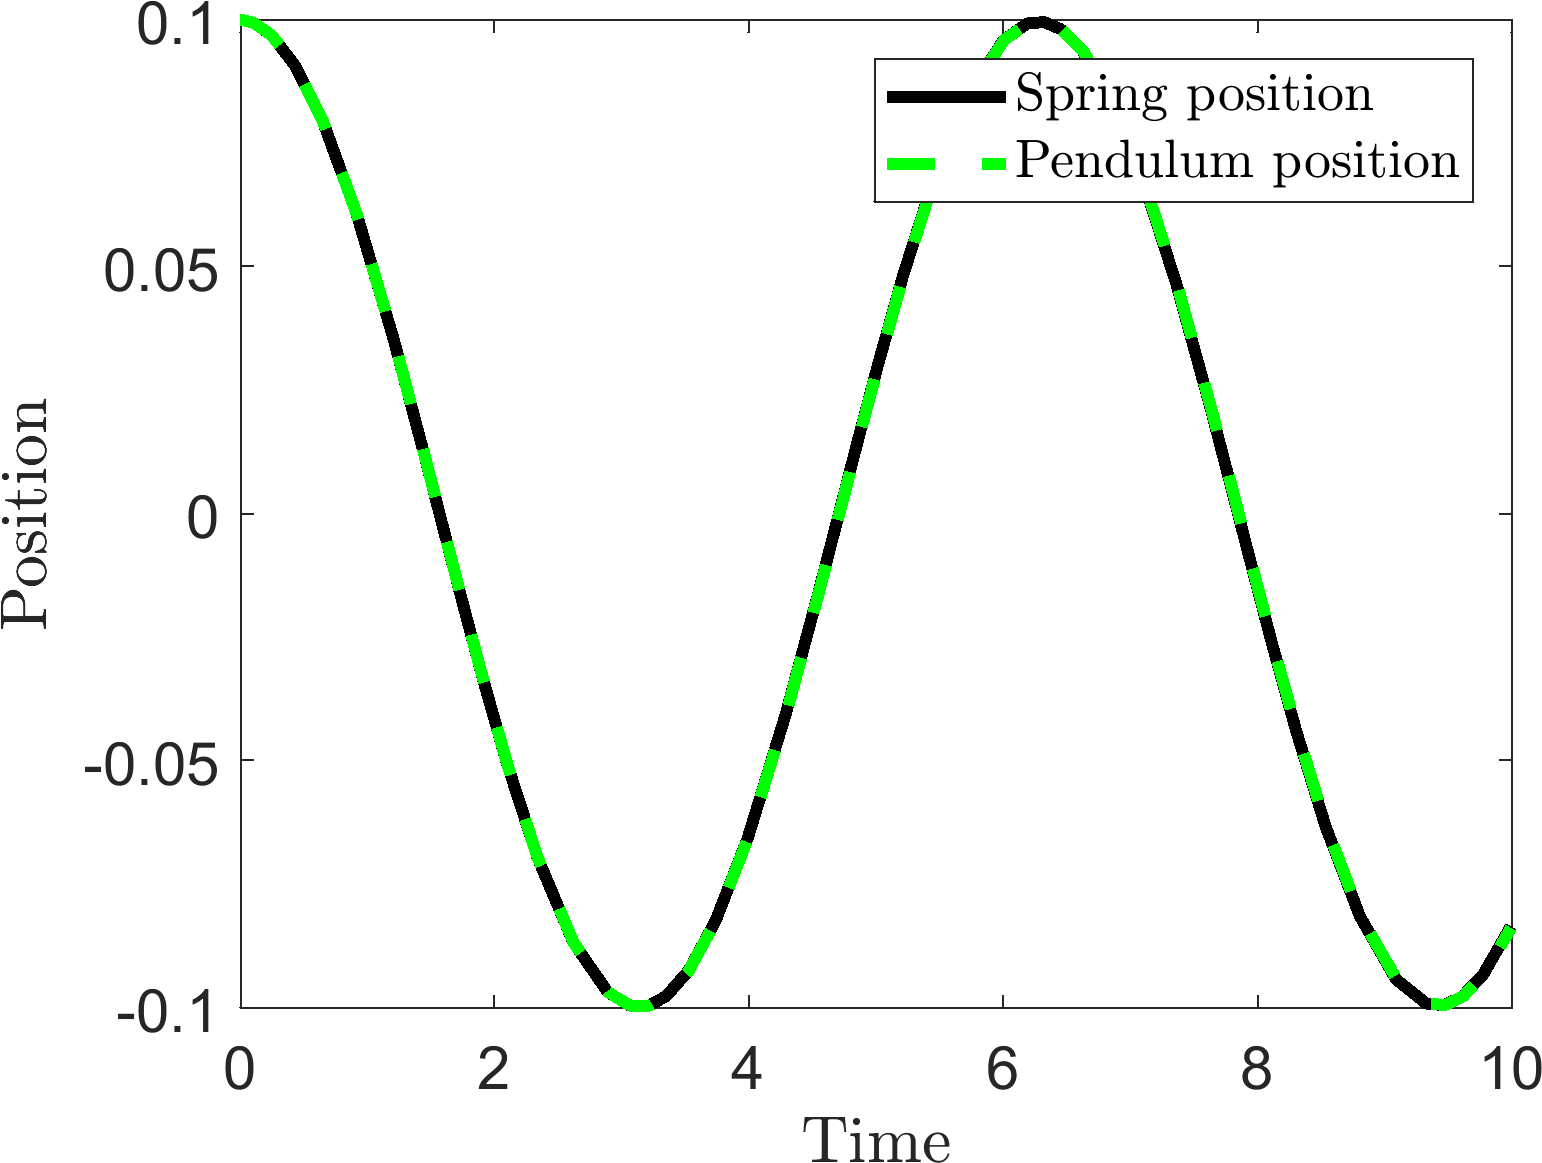
\includegraphics[width=\ttp]{../Pictures/Comparing_pendulums_IC_1.png}}
%\subfigure[\label{IC_1}]{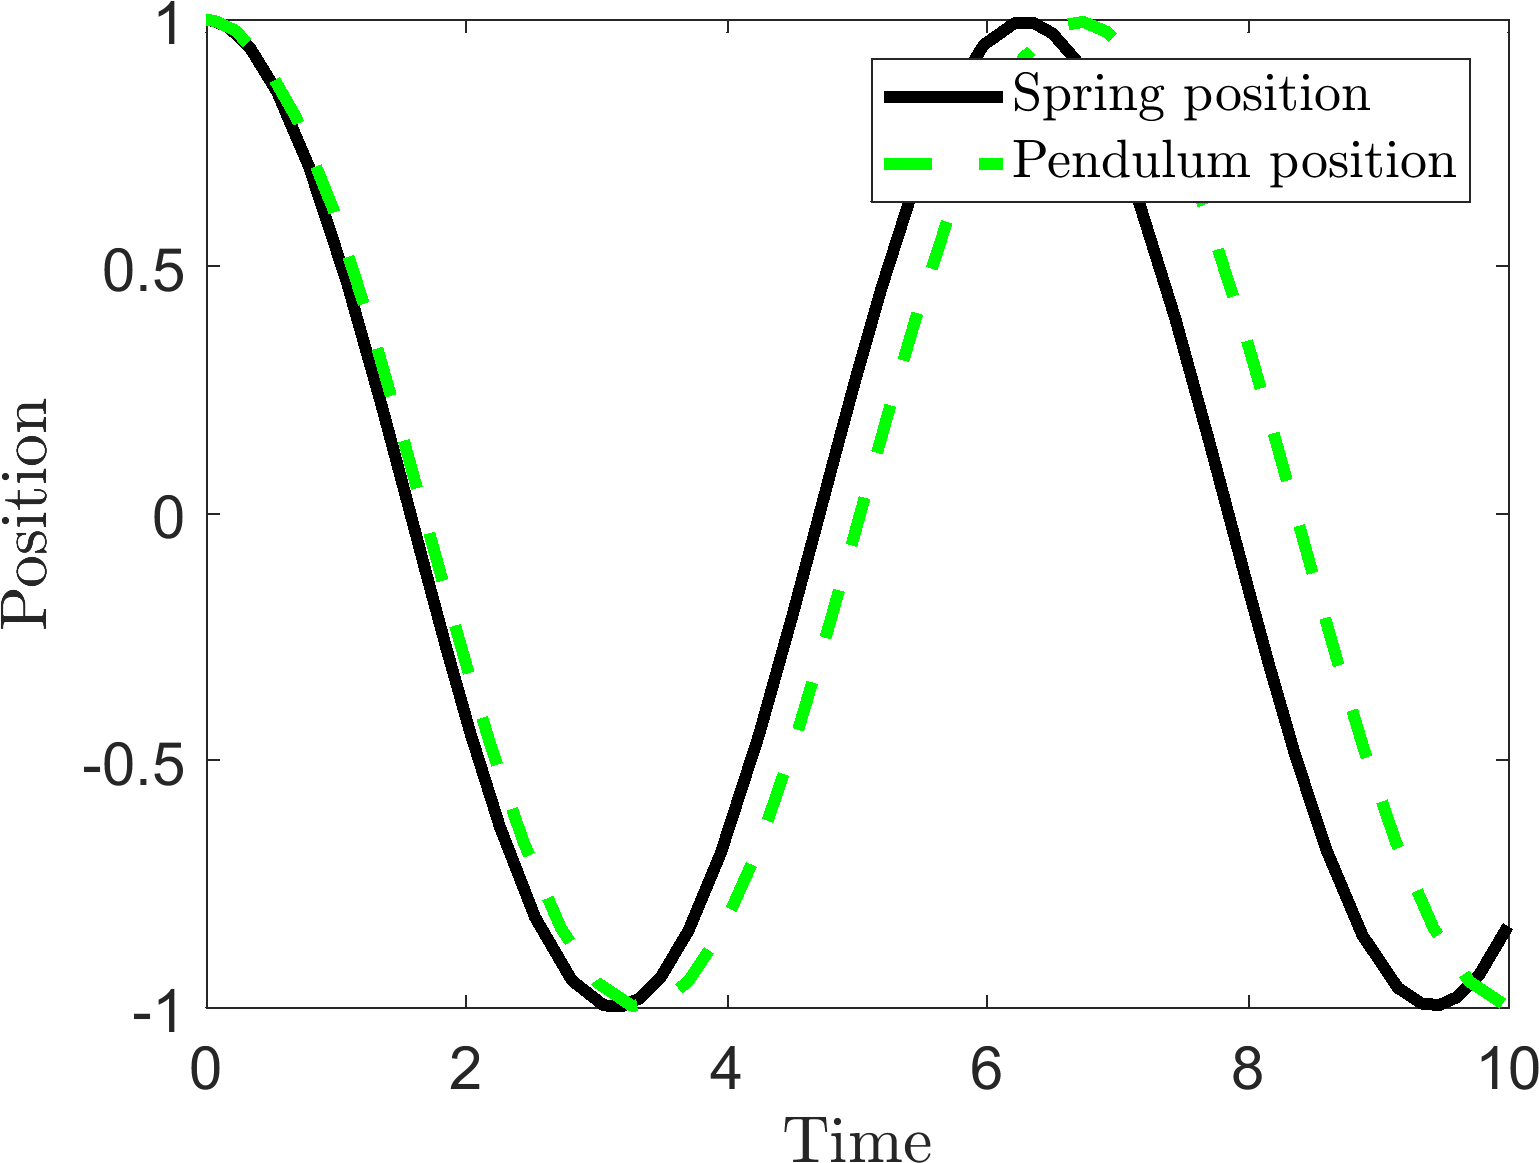
\includegraphics[width=\ttp]{../Pictures/Comparing_pendulums_IC_10.png}}
%\caption{\label{Different_ICs}Comparing \eqns{Spring_eqn}{Bob_eqn} with initial conditions (a) $y=0=\theta$ and (b) $y=1=\theta$. Parameter values $r=g=k=m=1$.}
%\end{figure}
%
%
%\begin{example}[frametitle=Zombies]\label{Zombies}
%Humans, $H$ and zombies, $Z$ interact through the following three interactions \see{Zombie_picture}]:
%\end{example}
%\begin{figure}[!!!h!!!tb]
%\centering
%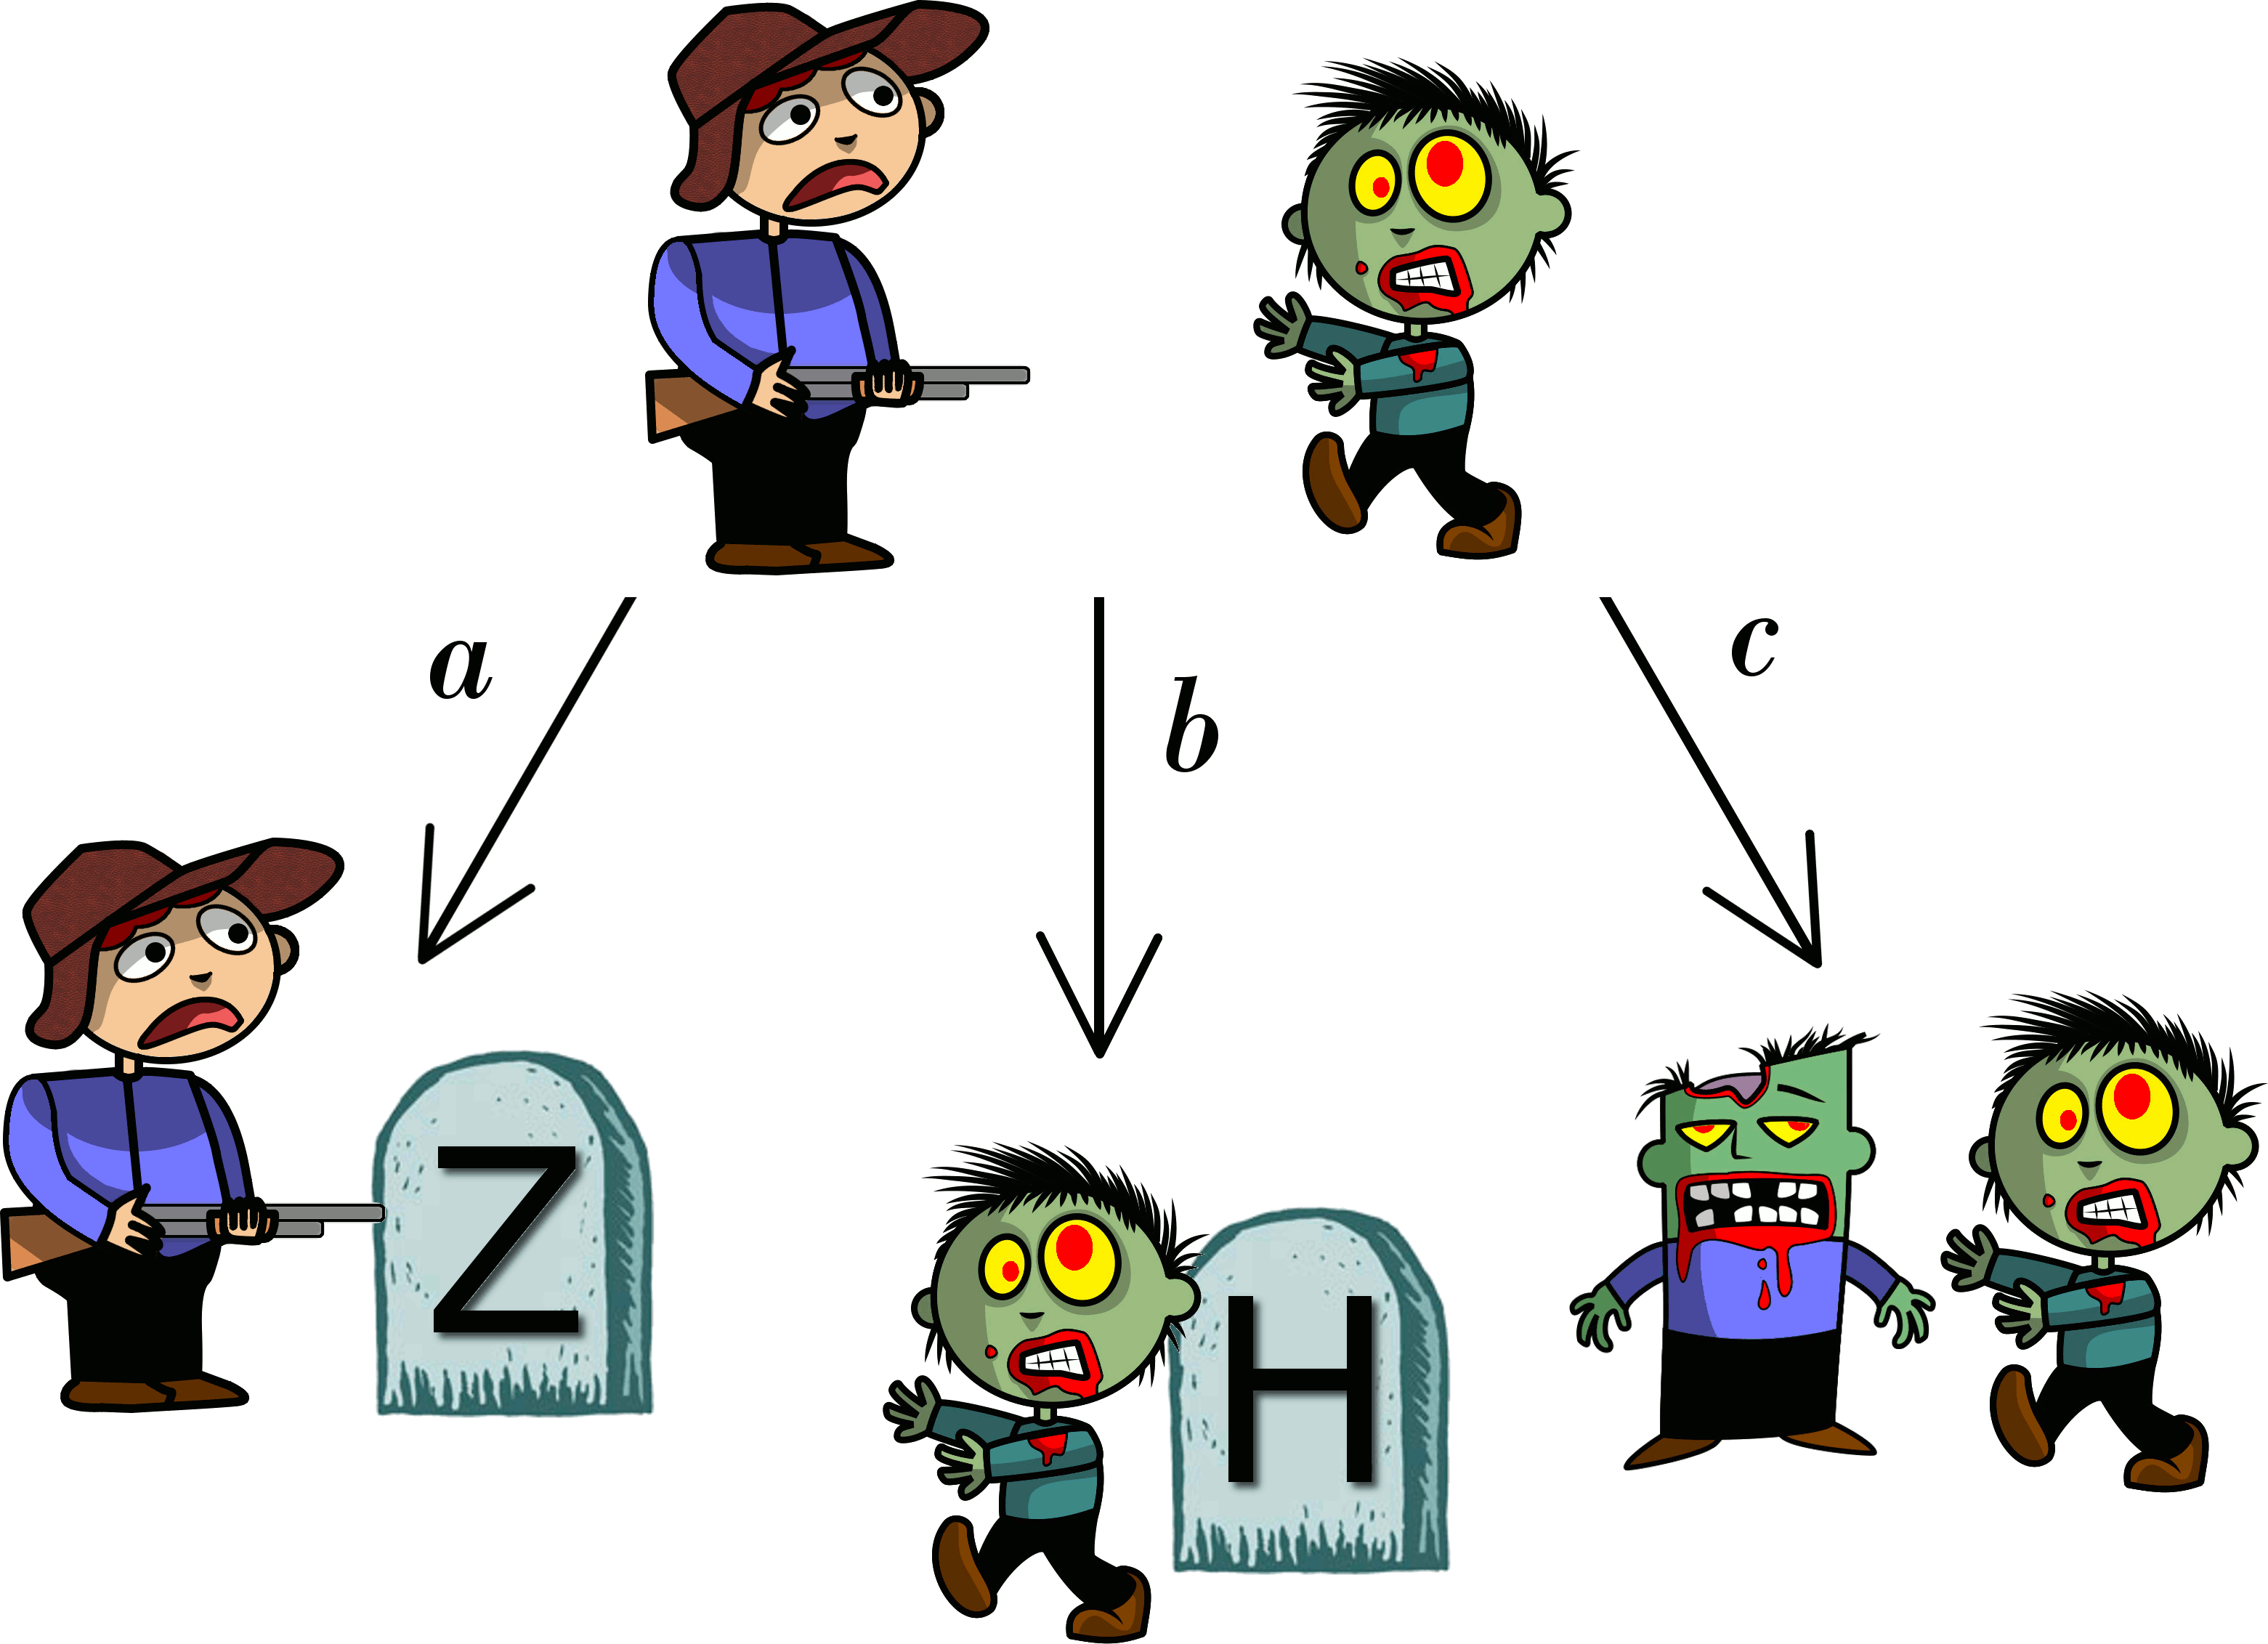
\includegraphics[width=\tp]{../Pictures/Zombies.png}
%\caption{\label{Zombie_picture} Possible outcomes of human-zombie interactions.}
%\end{figure}

\section{Check list}
By the end of this chapter you should be able to:
\begin{todolist}
\item non-dimensionalise a system of equations using direct substitution, or the arrow method;
\item demonstrate that the derived scales have the correct dimension;
\item demonstrate that remaining parameter groupings are non-dimensional;
\end{todolist}





\include{Stationary_states_and_stability}
\include{Stability_of_ODE_systems}
\include{Phase_plane_analysis}
\include{Putting_it_all_together}




%\bibliography{/mi/share/scratch/Woolley/PDFs/Thesis}{}
%\bibliography{C:/Users/woolley.35/Dropbox/Bibel_no_web}{}
%\bibliography{../Bibel_no_web}{}
\bibliographystyle{unsrtnat}
\end{document}